\documentclass[oneside, final, 12pt]{article}

\pagestyle{plain}

\usepackage{a4wide}
\usepackage[utf8]{inputenc}
\usepackage[russian]{babel}
\usepackage{vmargin}
\setpapersize{A4}
\setmarginsrb{2cm}{1.5cm}{1cm}{1.5cm}{5pt}{5mm}{5pt}{13mm}
\usepackage{indentfirst}
\usepackage{graphicx}

\usepackage{amsmath}
\usepackage{amsfonts}
\usepackage{amsthm}
\usepackage{amssymb}

\def\Var{{\mathbb{V}\textrm{ar}}\,}
\def\E{{\mathbb{E} }\,}
\def\Cov{{\mathbb{C}\textrm{ov}}\,}
\def\P{{\mathbb{P} }}
\def\Q{{\mathbb{Q} }}
\def\a{{\textrm{a}}}
\def\b{{\textrm{b}}}

\DeclareMathOperator*{\Argmax}{Arg\,max}

\newtheorem{theorem}{Теорема}
\newtheorem{definition}{Определение}
\newtheorem{statement}{Утверждение}
\newtheorem{consequence}{Следствие}
\newtheorem{remark}{Замечание}

\usepackage{subcaption}
\usepackage{caption}


\begin{document}

\thispagestyle{empty}

\begin{center}
\ \vspace{-3cm}

\includegraphics[width=0.5\textwidth]{msu.pdf}\\
{\scshape Московский государственный университет имени М.~В.~Ломоносова}\\
Факультет вычислительной математики и кибернетики\\
Кафедра системного анализа

\vfill

{\LARGE Отчёт по практикуму}

\vspace{1cm}

{\Huge\bfseries <<Стохастический анализ и моделирование>>}
\end{center}

\vspace{1cm}

\begin{flushright}
    \large
    \textit{Студент 415 группы}\\
    И.~А.~Кулешов
    \vspace{5mm}
    
    \textit{Руководитель практикума}\\
    к.ф.-м.н, доцент С.~Н.~Смирнов
\end{flushright}

\vfill

\begin{center}
Москва, 2019
\end{center}

\newpage
\tableofcontents

\newpage
\section{Задание 1}

\subsection{Постановка задачи}
    \begin{enumerate} 
        \item Реализовать генератор схемы Бернулли с заданной вероятностью успеха $p$. 
        		На основе генератора схемы Бернулли построить датчик для биномиального распределения.
        \item Реализовать генератор геометрического распределения. 
        		Проверить для данного распределения свойство отсутствия памяти.
        \item Рассмотреть игру в орлянку -- бесконечную последовательность независимых испытаний
			 с бросанием правильной монеты. Выигрыш $S_n$ определяется как сумма по
			всем $n$ испытаниям значений $1$ или $-1$ в зависимости от выпавшей стороны.
			Проиллюстрировать (в виде ломаной) поведение нормированной суммы $Y(i) = S_i/\sqrt{n}$
			как функцию от номера испытания $i = 1,\ldots, n$ для одной отдельно взятой траектории. 
			Дать теоретическую оценку для $Y(n)$ при $n\rightarrow\infty$.
    \end{enumerate}
\subsection{Решение задачи}
\subsubsection{Пункт 1}
    \begin{definition}
    Схемой Бернулли с заданной вероятностью успеха $p$ называется эксперимент, удовлетворяющих следующим свойствам:
        \begin{enumerate}
            \item Отсутствие взаимного влияния между испытаниями в эксперименте.
            \item Воспроизводимость испытаний (испытания производятся в сходных условиях).
            \item В каждом испытании можно выделить признак, который может проявиться с определенной
		вероятностью $p$.
        \end{enumerate}
    \end{definition}
    
    \begin{definition}
        Случайная величина $X$, которая принимает значение 1, когда признак реализуется, и 0, когда он не 
		реализуется, в схеме Бернулли из 1 испытания называется бернуллиевской.
        Обозначение: $X \sim Bern(p)$.
    \end{definition}
    В таком случае мы можем реализовать генератор схемы Бернулли на основе датчика случайной 
	величины, распределенной равномерно $\xi \sim U[0;1]$ следующим образом:
    $$
	    X =
			\left \{ \begin{aligned} 
					       	& 1,	    &\quad{\xi \in  [0, p)}, \\ 
					       	& 0,    &\quad{\xi \in  [1, p]}. 
	    			    \end{aligned} 
			\right.
	$$
	\begin{definition}
        Случайная величина
        $$Y = \sum_{k=1}^{n} X_k, \quad X_k \sim Bern(p), \quad k = \overline{1,n} $$ 
        имеет по определению биномиальное распределение с параметрами $n$ и $p$.
        \newline Обозначение: $Y \sim B(n,p).$ 
    \end{definition}
    Теоретическое распределение: $$\P(Y = k ) = C_n^k p^k (1-p)^{n-k}.$$
    \begin{figure}[h!]
		\centering
		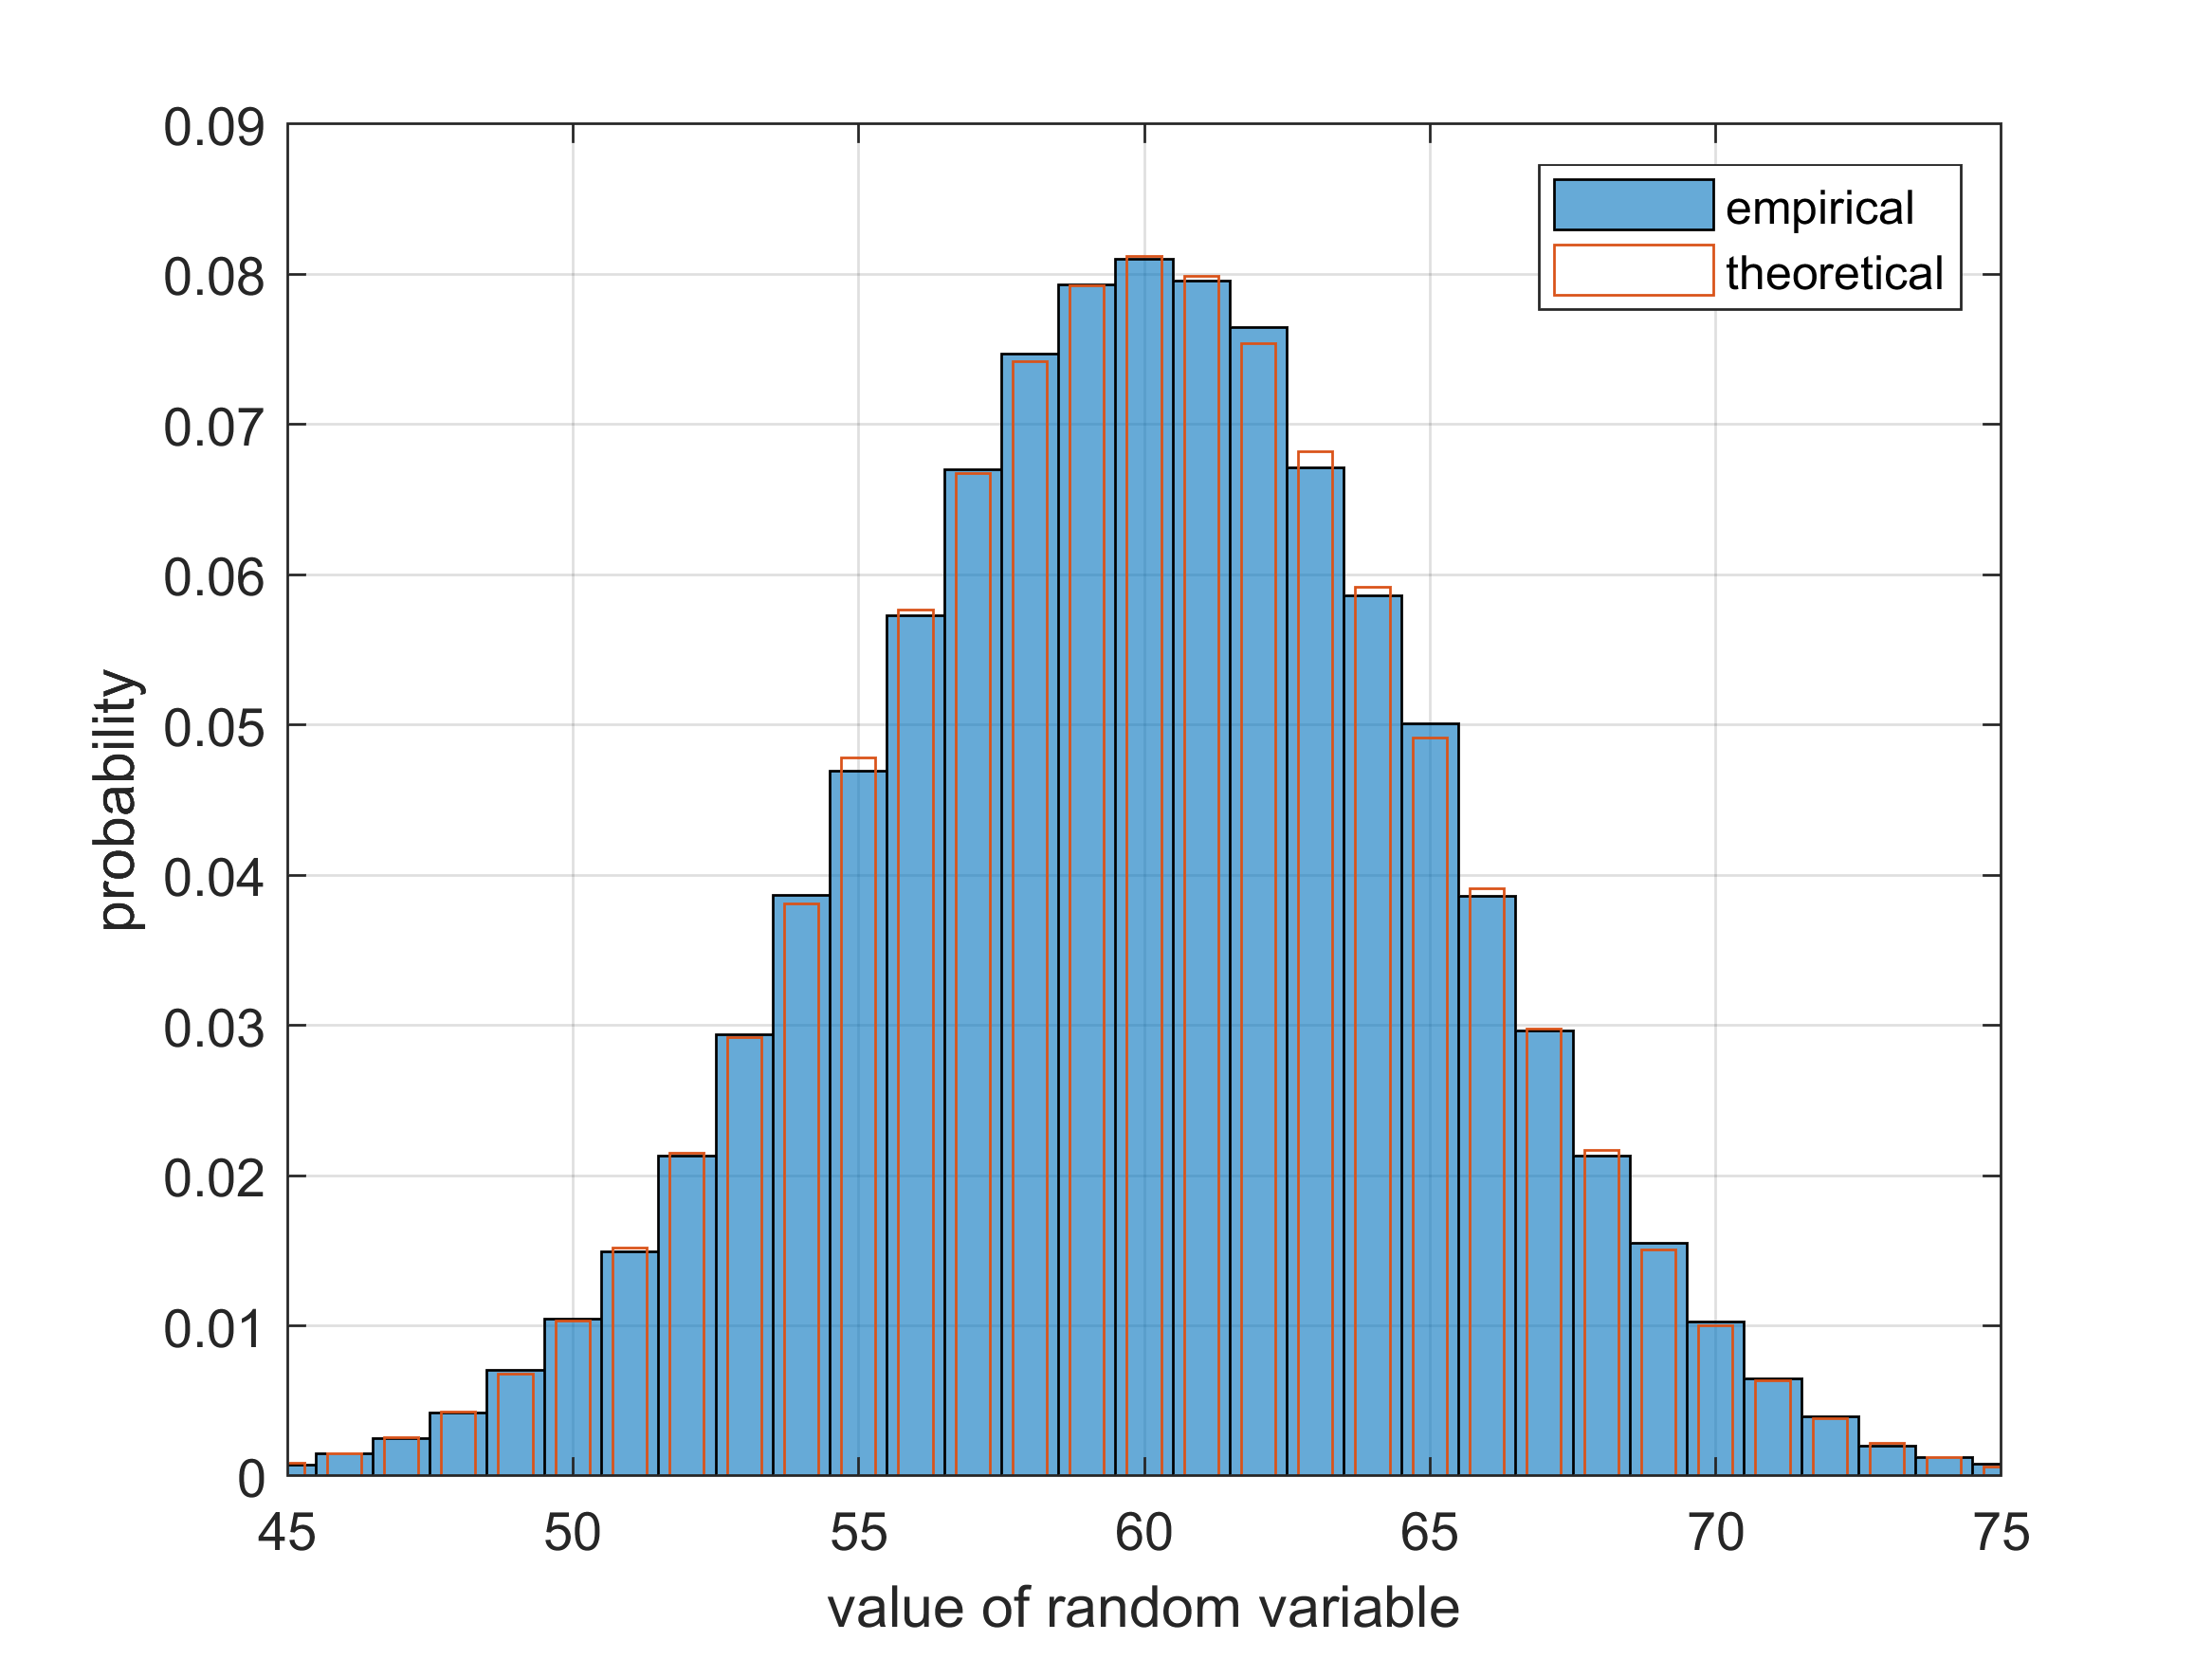
\includegraphics[width=0.6\textwidth]{../code/Task_1/pict/binom_vis_ex.png}
		\caption{Гистограмма биномиального распределения с параметрами $p$ = 0.6, $n$ = 100.
		\newline \centering  Размер выборки $10^5.$}
    \end{figure}

\subsubsection{Пункт 2}
    \begin{definition}
        Распределение случайной величины, равной количеству неудач до появления
		первого успеха в схеме Бернулли с параметром $p$, называется геометрическим распределением.
        	Обозначение: $Z\sim Geom(p).$ 
    \end{definition}

    Теоретическое распределение: $$\P(Z=k) = (1-p)^{k}p.$$
    \begin{figure}[h!]
		\centering
		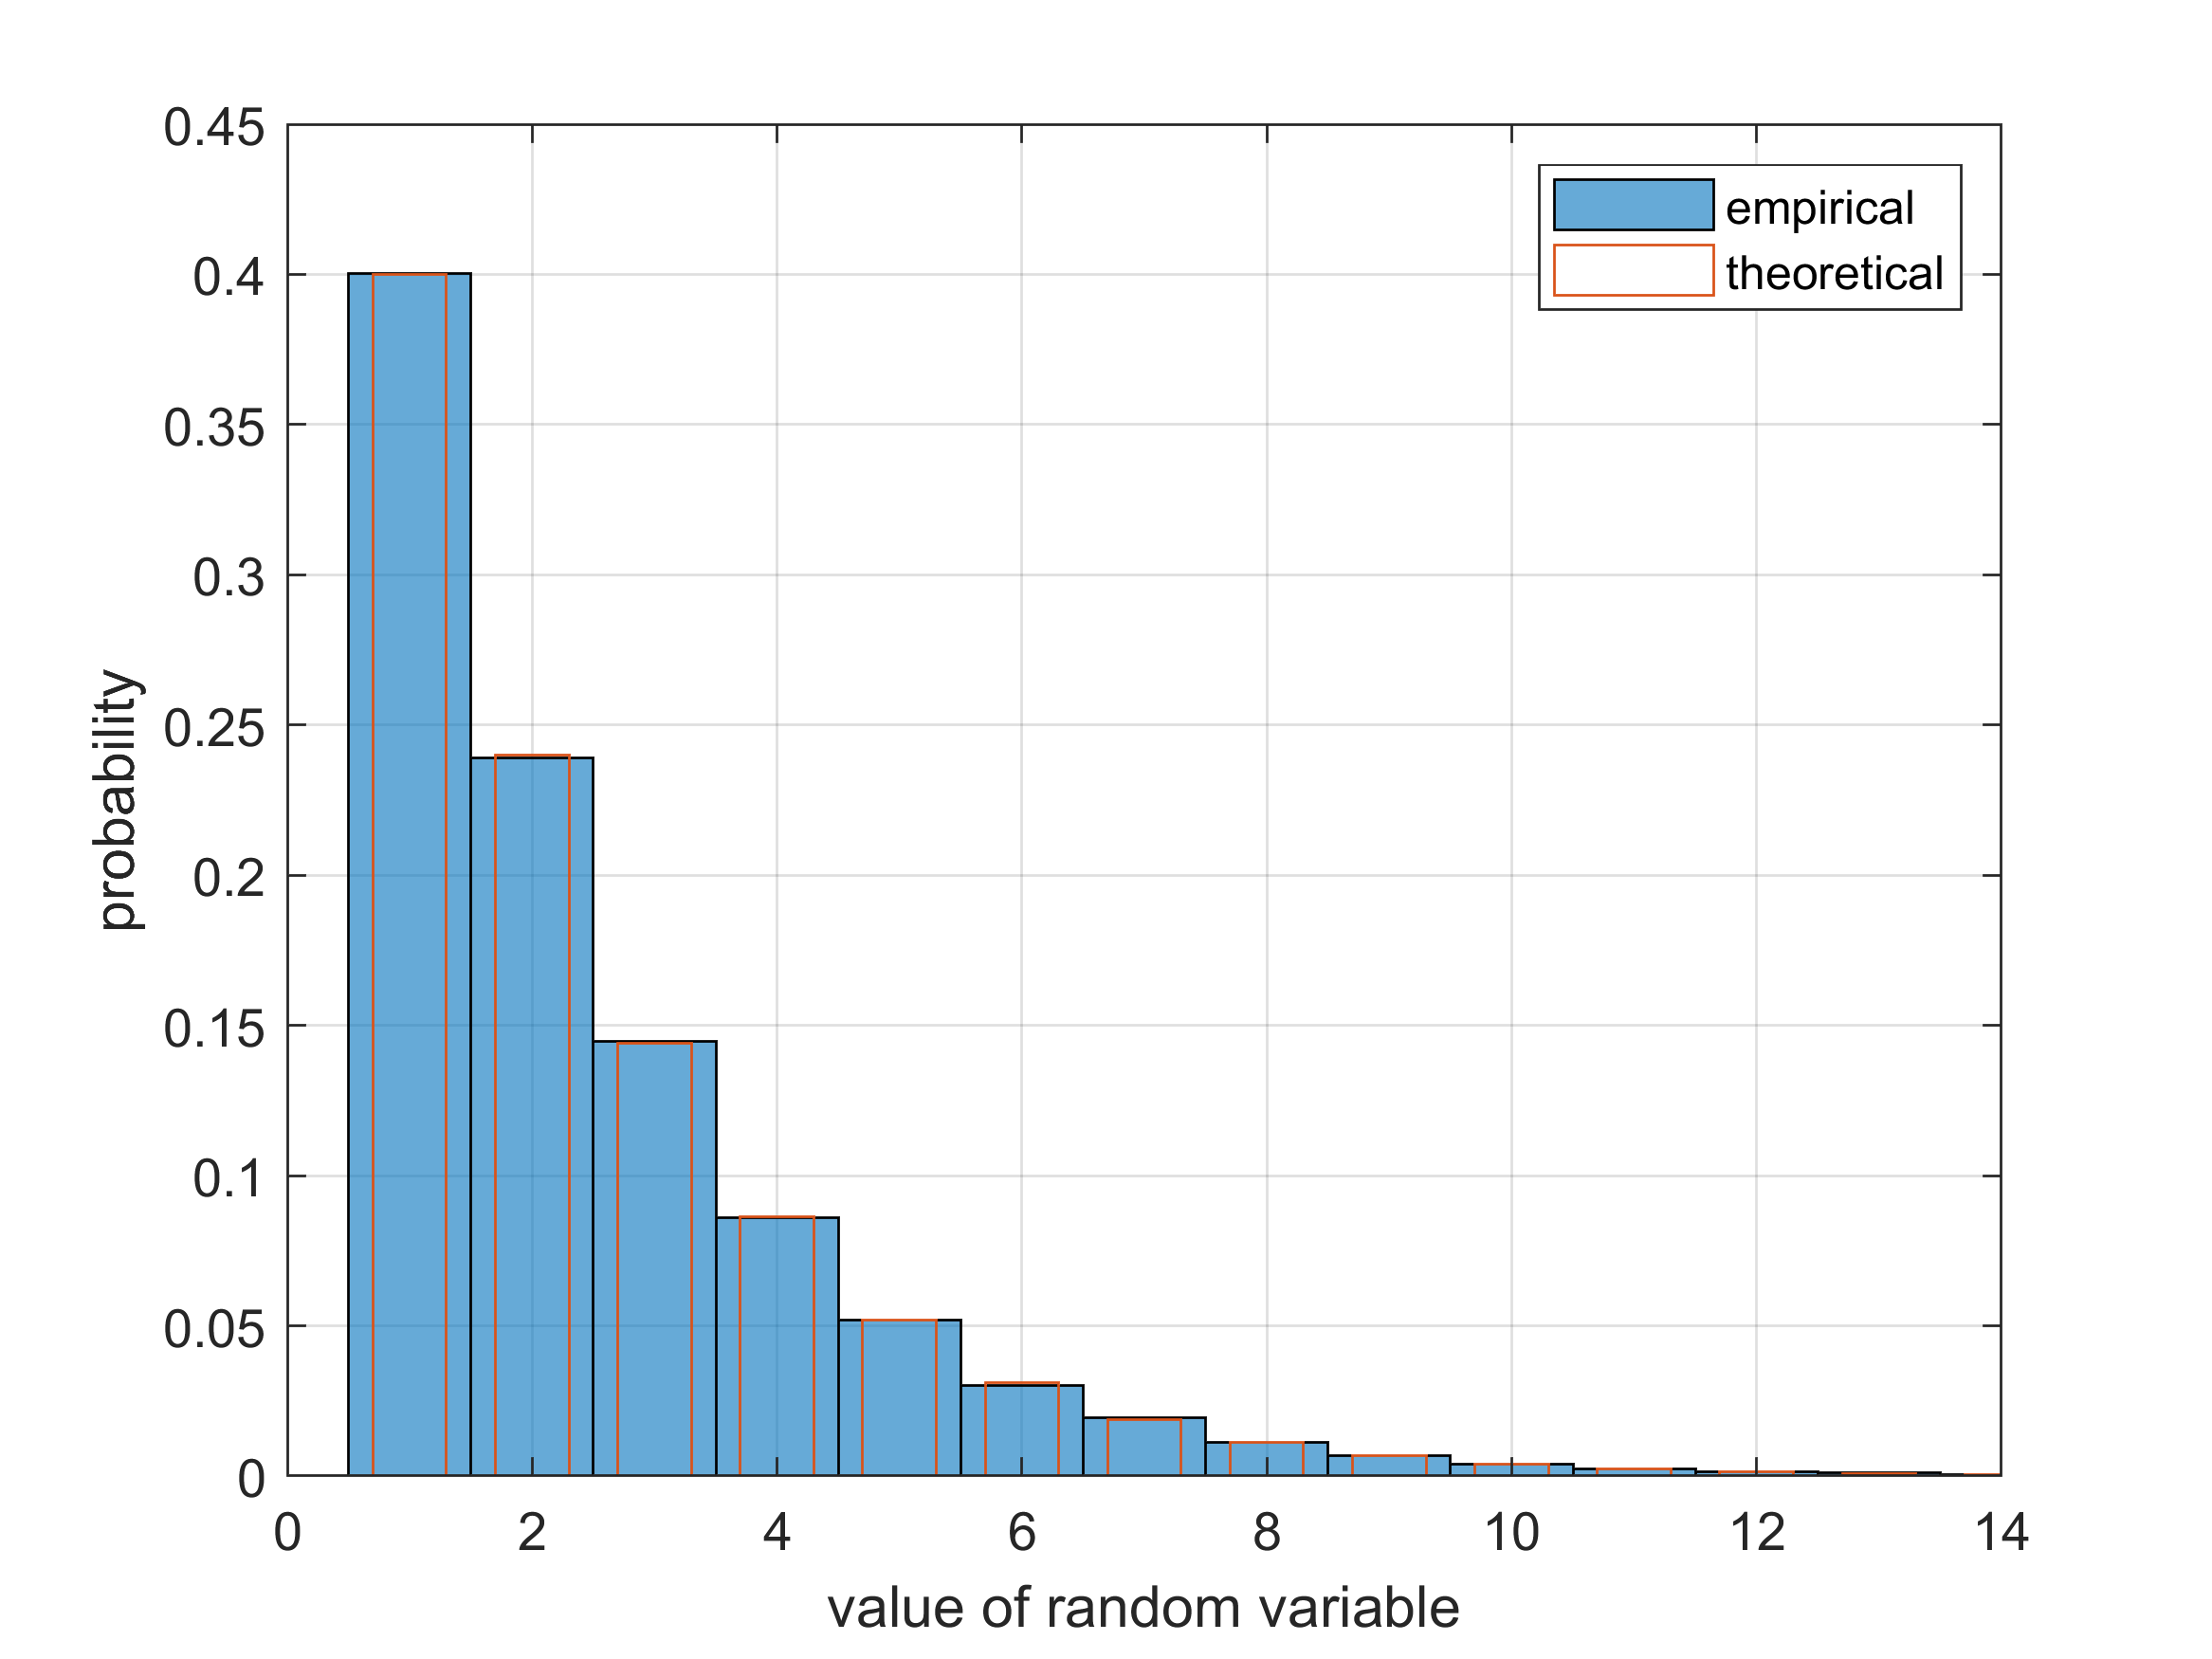
\includegraphics[width=0.6\textwidth]{../code/Task_1/pict/geom_vis_ex.png}
		\caption{Гистограмма геометрического распределения с параметром $p$ = 0.4.
		\newline \centering  Размер выборки $10^5$.}
    \end{figure}

    \begin{statement}
    Если $Z \sim Geom(p)$, то выполняется 
            $$\P(Z > m + n \mid Z \geqslant m) =\ P(Z > n)$$ для любых целых неотрицательных n и m. 
    \end{statement}

    \begin{proof}
        \begin{multline}
          \P(Z > m + n \mid Z \geqslant m) = \frac{\P(Z > m + n, Z \geqslant m)}{\P(Z\geqslant m)} =\\
            = \frac{\P(Z >  m + n)}{\P(Z \geqslant m)}  =
            \frac{(1-p)^{m+n+1}}{(1-p)^m} = 
                (1-p)^{n+1} = P(Y > n)
        \end{multline}
    \end{proof}
    Это называют свойством отсутствия памяти у геометрического распределения.
    \begin{figure}[h!]
		\centering
		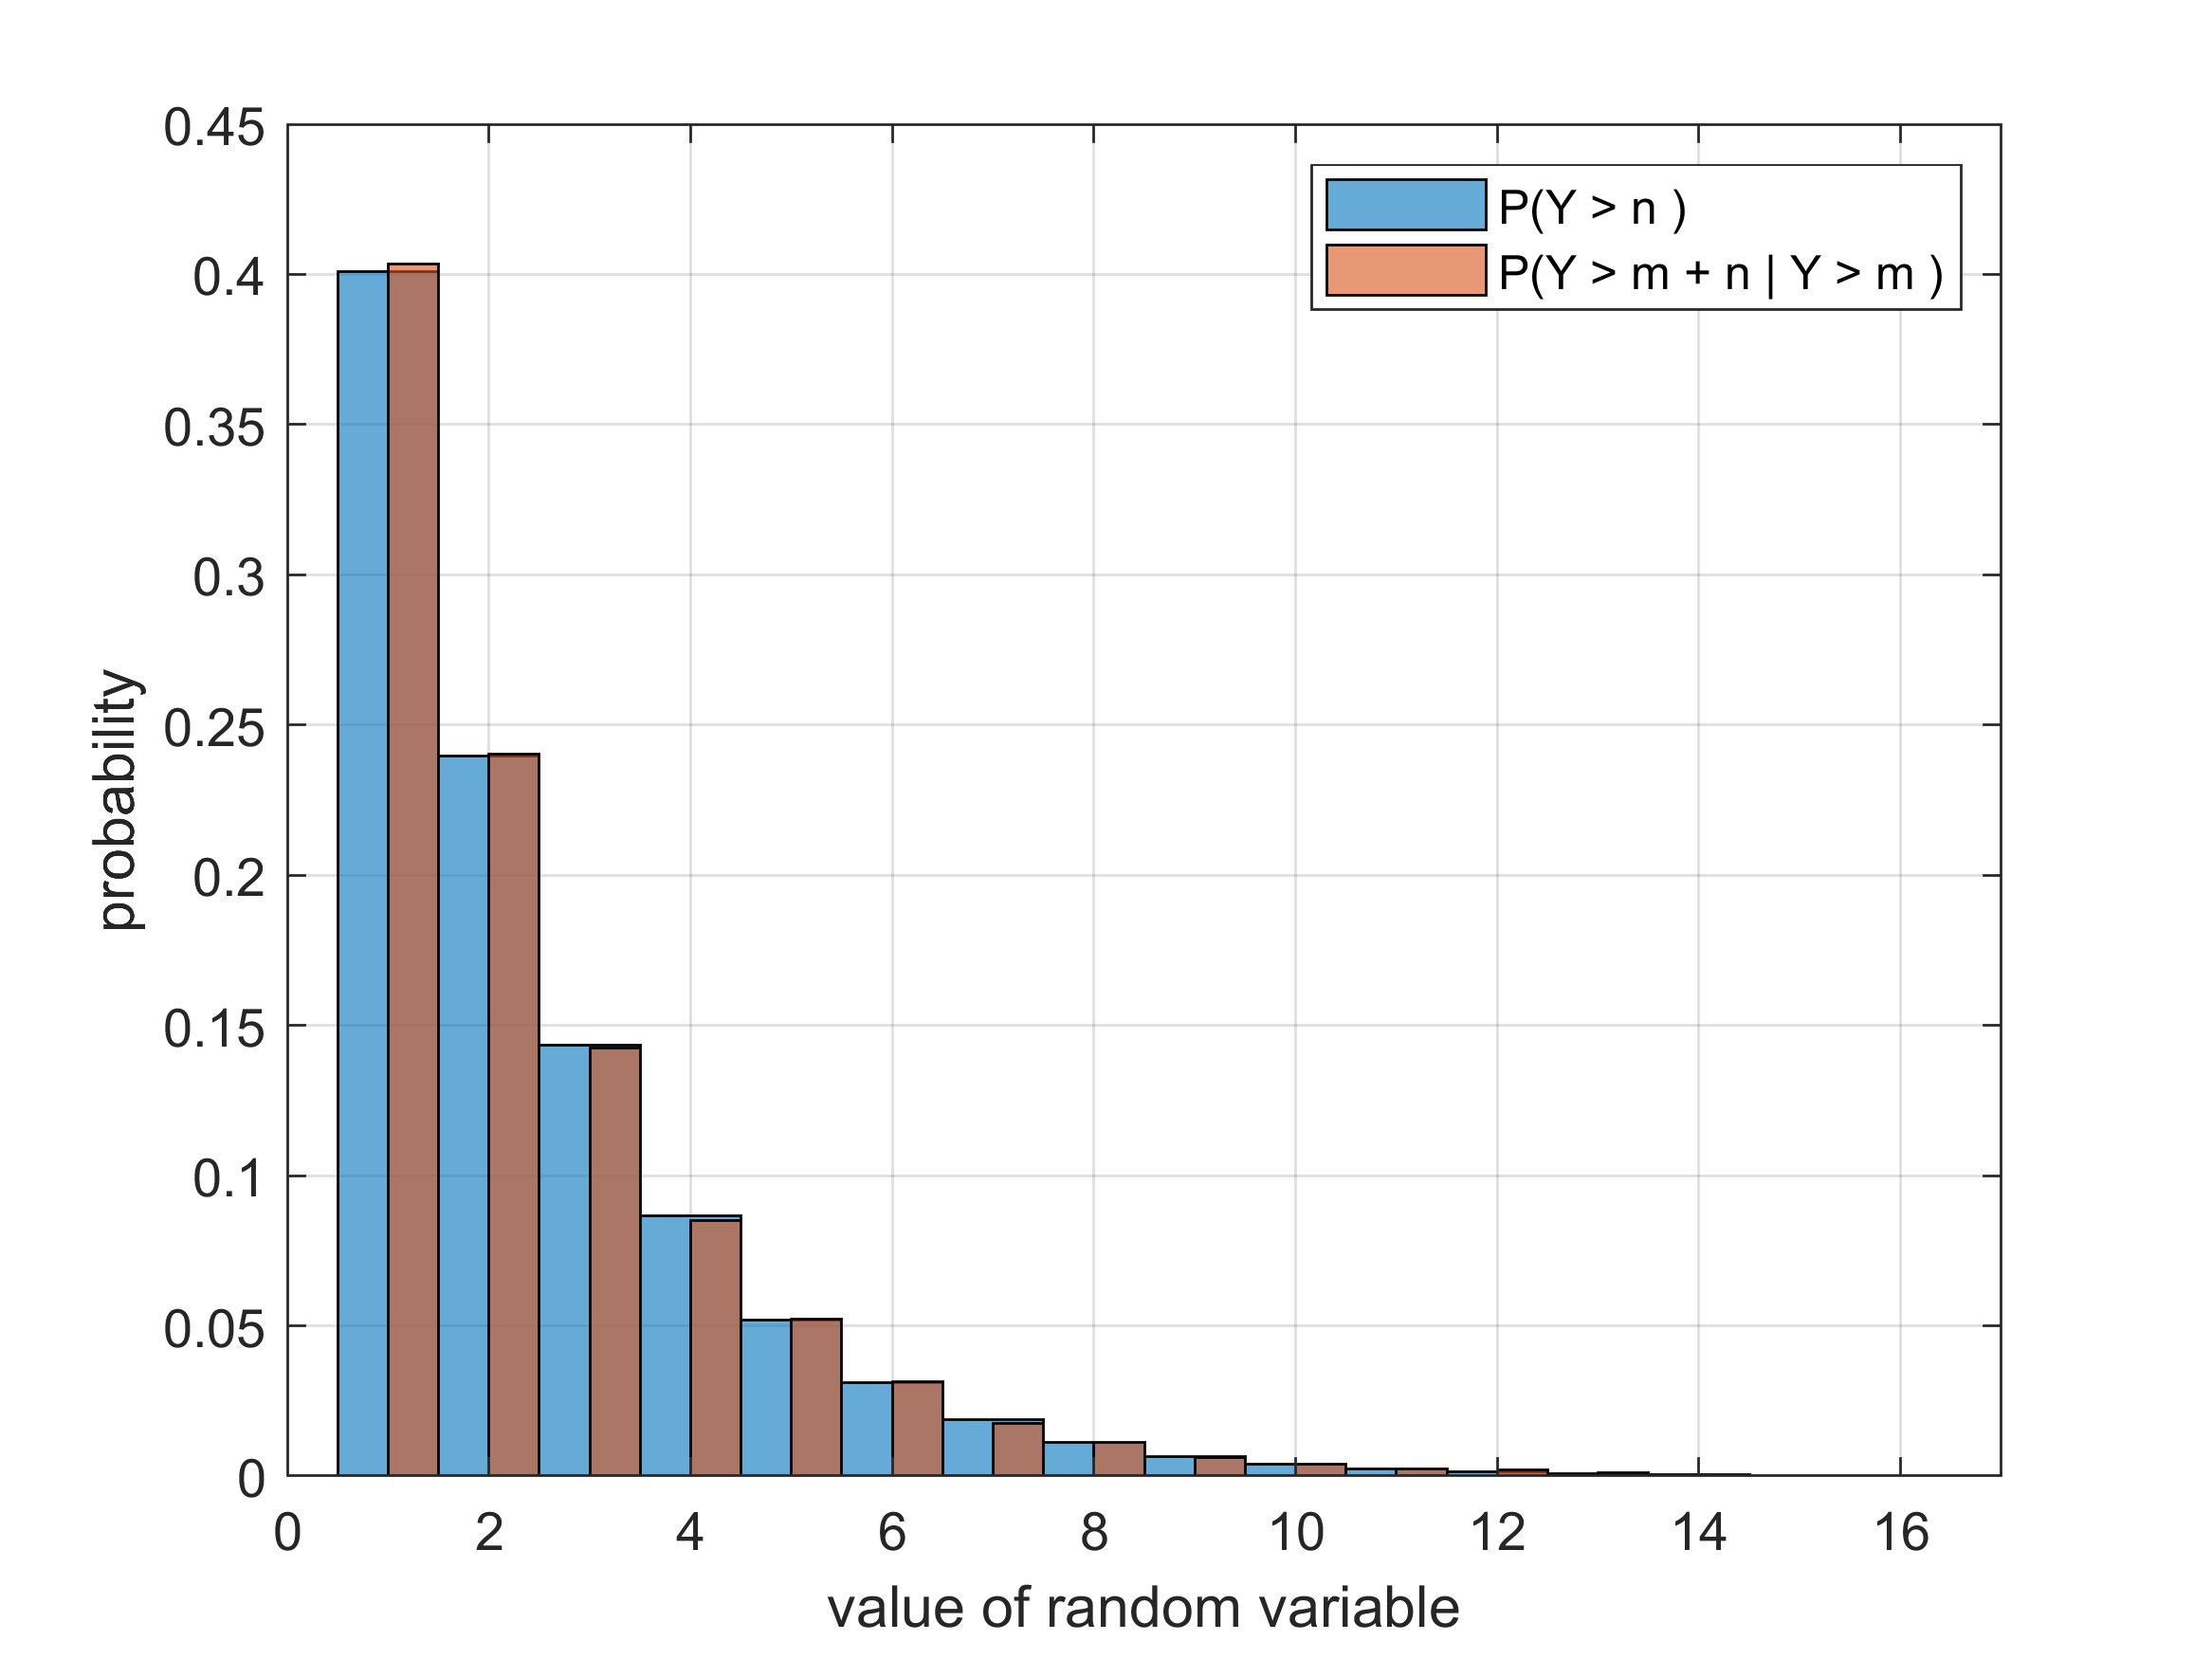
\includegraphics[width=0.6\textwidth]{../code/Task_1/pict/mmls_prop_ex.png}
		\caption{Свойство отсутствия памяти геометрического распределения. 
		\newline \centering  Параметры: p = 0.4, n = 1 и m = 6, размер выборки $10^5$.}
    \end{figure}
    
\subsubsection{Пункт 3}
    Рассмотрим игру в орлянку. 
    \begin{theorem}{\textbf{ЦПТ}}
    \newline
        Пусть $X_1, X_2, \ldots, X_n$ --- последовательность невырожденных н.о.р.с.в.  
		с $\E X_1^2<\infty$, $S_n = X_1 + \ldots + X_n$. Тогда для $\forall x \in \mathbb{R}$ имеем
        $$
            \P\left\{\frac{S_n-\E S_n}{\sqrt{\Var S_n}}\leqslant x\right\} 
            \xrightarrow[]{n \rightarrow \infty} \Phi(x) = \frac{1}{\sqrt{2\pi}}
                                \int\limits^{x}_{-\infty}e^{-\frac{z^2}{2}}dz.
        $$
    \end{theorem}
    \begin{figure}[h!]
		\centering
		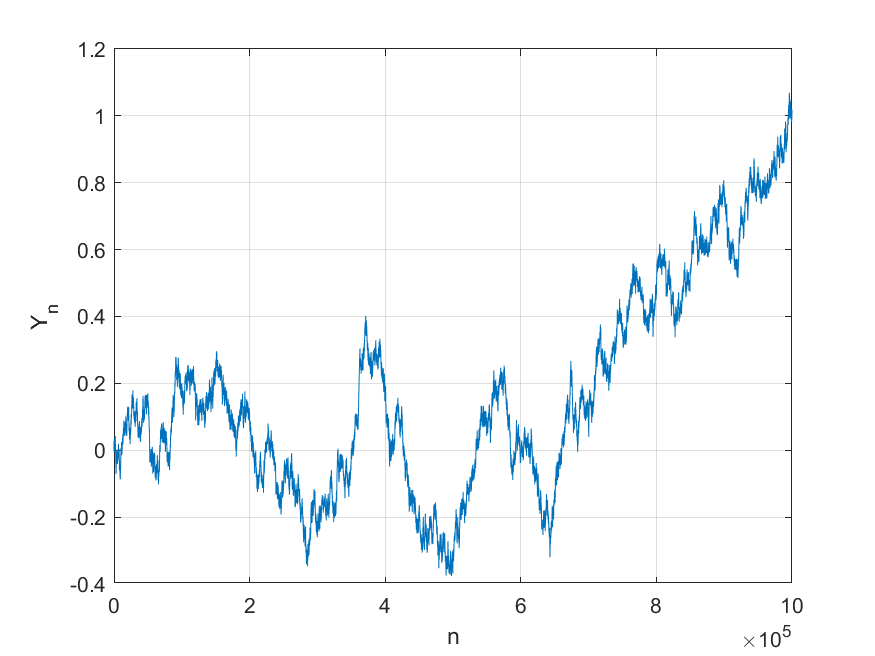
\includegraphics[width=0.6\textwidth]{../code/Task_1/pict/h_t_ex.png}
		\caption{Одна из траекторий игры в орлянку при $10^5$ бросаний монеты. }
    \end{figure}
    В нашем случае $\E X_1 = a = 0 $, $\Var X_1 = \sigma^2 = 1$. 
    \newline Оценим $S_n/\sqrt{n}$. По ЦПТ получаем:
    $$
        \P\left\{\left|\frac{S_n}{\sqrt{n}}\right| \leqslant 
            t_{\frac{1+\gamma}{2}} \right\} = \gamma
    $$
    По таблице квантилей нормального распределения найдем значение $t_{\frac{1+\gamma}{2}}.$
    \newline Окончательно получим доверительный интервал с коэффициентом доверия $\gamma= 0.95$ : 
        $$
			 -1.96 \leqslant \frac{S_n}{\sqrt{n}} \leqslant  1.96,
		$$
	что совпадает с иллюстрацией.

\section{Задание 2}

\subsection{Постановка задачи}
    \begin{enumerate} 
        \item Построить датчик сингулярного распределения, имеющий в качестве функции распределения
	 	канторову лестницу. С помощью критерия Колмогорова убедиться в корректности работы датчика. 
        \item Для канторовых случайных величин проверить свойство симметричности относительно 
			$\frac{1}{2}$ ($X$ и $1-X$ распределены одинаково) и самоподобия относительно деления 
			на $3$ (условное распределение $Y$ при условии $Y \in [0,1/3]$ совпадает 
			с распределением $\frac{Y}{3}$) с помощью критерия Смирнова.
        \item Вычислить значение математического ожидания и дисперсии для данного распределения.
			Сравнить теоретические значения с эмпирическими для разного объема выборок.
			Проиллюстрировать сходимость.
    \end{enumerate}
\subsection{Решение задачи}
\subsubsection{Пункт 1}
	
	\begin{definition}
		Функция распределения называется сингулярной, если она непрерывна и ее множество
		точек роста имеет нулевую меру Лебега.
	\end{definition}
	Заметим, что канторово множество можно представить как множество всех $x \in [0, 1]$,
	представление которых в троичной системе счисления содержит только цифры 0 и 2.
	Соответсвенно их можно сгенерировать следующим образом:
	$$
		x = \sum\limits_{k=1}^{\infty} \dfrac{2 \alpha_k}{3^k},
	$$
	где $\alpha_k \sim Bern(0.5)$. Значения функции Кантора $C(x)$ будут определяться
	путем замены всех цифр 2 числа $x$ в троичной системе на 1 
	и трактовкой полученного числа в двоичной системе счисления.
	\begin{figure}[h!]
		\centering
		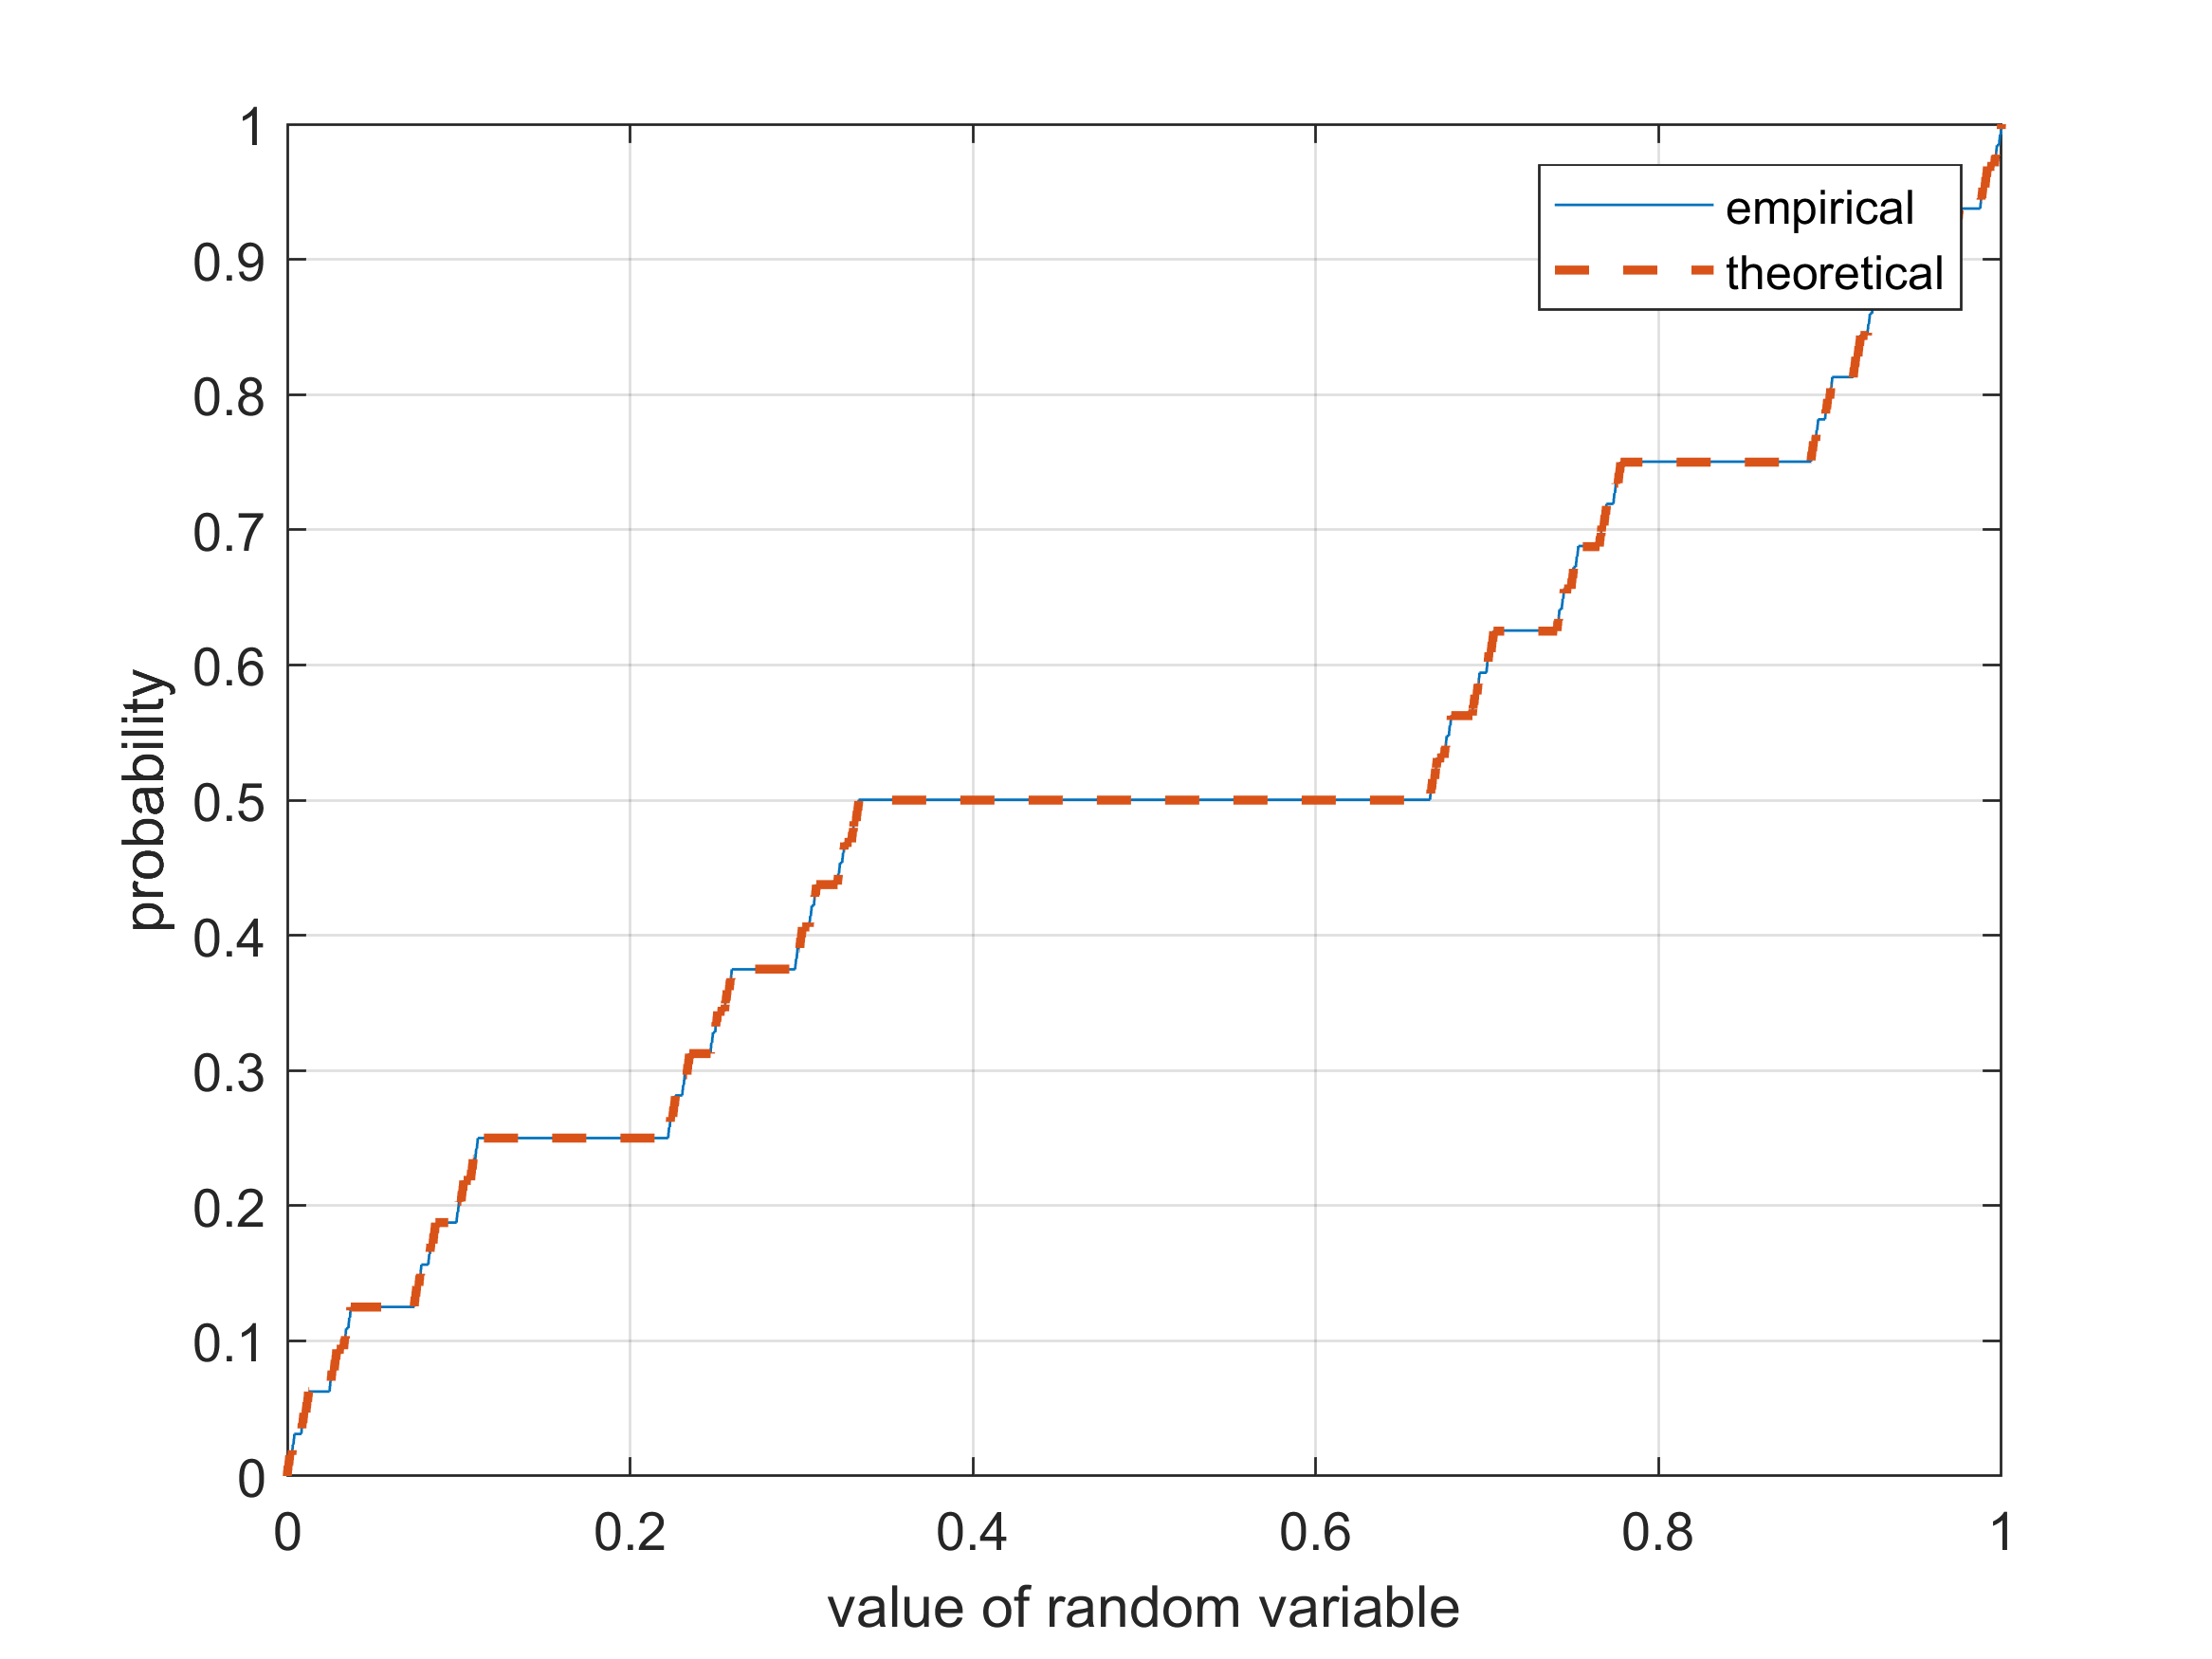
\includegraphics[width=0.6\textwidth]{../code/Task_2/pict/cant_vis_ex.png}
		\caption{Каторова функция при $n=10^6$. }
    \end{figure}
	
	Пусть у нас есть эмпирическая функция распределения $F_n(x)$,
	построенная по выборке $X = (X_1, X_2, \ldots, X_n)$, и предполагаемая функция
	распределения $F(x)$. Статистику критерия Колмогорова определим
	следующим образом: $$D_n = \sup\limits_{x}|F(x) - F_n(x)|.$$ 
		\textbf{Принятие решения по критерию Колмогорова:}

	Если $p_{value}$, равное $p = 1 - K(\sqrt {n}D_{n})$,
	где $K(x)$ --- это функция распределения Колмогорова, превышает уровнь
	значимости $\alpha$, то нулевая гипотеза $H_{0}$ 
	о соответствии закону $F(x)$ принимается. 
	Иначе гипотеза отвеграется на уровне $\alpha$.

	\begin{table}[h!]
	\begin{center}
		\begin{tabular}{|c|c|c|c|}
			\hline $N$ & частота принятия гипотезы \\ \hline
				$10^2$ & 0.96  \\ \hline
				$10^3$ & 0.948 \\ \hline
		\end{tabular}
		\caption{Результаты проверки сингулярности генрируемого распределения при $\alpha = 0.05$.}
	\end{center}
	\end{table}
	
\newpage
\subsubsection{Пункт 2}
	
		Пусть случайная величина $Y= \sum\limits_{k=1}^{\infty}\dfrac{2\alpha_k}{3^k}$, 
	где $\alpha\sim Bern(0.5)$. Рассмотрим случайную величину $1-Y$, чтобы показать симметрию
	распределения относительно $\frac{1}{2}$:
	$$
		1- Y= 1- \sum\limits_{k=1}^{\infty}\dfrac{2\alpha_k}{3^k} =
					 \sum\limits_{k=1}^{\infty}\dfrac{2}{3^k} - \sum\limits_{k=1}^{\infty}\dfrac{2\alpha_k}{3^k} = 
				    \sum\limits_{k=1}^{\infty}\dfrac{2(1-\alpha_k)}{3^k} =
					 \sum\limits_{k=1}^{\infty}\dfrac{2\beta_k}{3^k}, 
	$$
	где $\beta_k \sim Bern(0.5)$. Это значит, что cлучайные величины $1-Y$  и $Y$ распределены одинаково. 

	Проверим справдливость данного свойства при помощи критерия Смирнова. 
	Пусть у нас есть две эмпирические функции распределения $F_{1,n}(x)$ и $F_{2,m}(x)$ ,
	построенные по выборкам $X_1 = (x_1, x_2, \ldots, x_n)$ и $X_2 = (x_1, x_2, \ldots, x_m)$ соответственно.
	Статистику критерия Смирнова определим следующим образом:
	$$D_{n,m} = \sup\limits_{x}|F_{1,n}(x) - F_{2,m}(x)|.$$
	\textbf{Принятие решения по критерию Смирнова:}

	Если $p_{value}$, равное $p = 1 - K\left(\sqrt{\dfrac{nm}{n+m}}D_{n,m}\right)$,
	где $K(x)$ --- это функция распределения Колмогорова, превышает уровнь
	значимости $\alpha$, то нулевая гипотеза $H_{0}$ 
	об идентичности распределений выборок $X_1$ и $X_2$ принимается. 
	Иначе гипотеза отвеграется на уровне $\alpha$.
		
	\begin{figure}[h!]
		\centering
		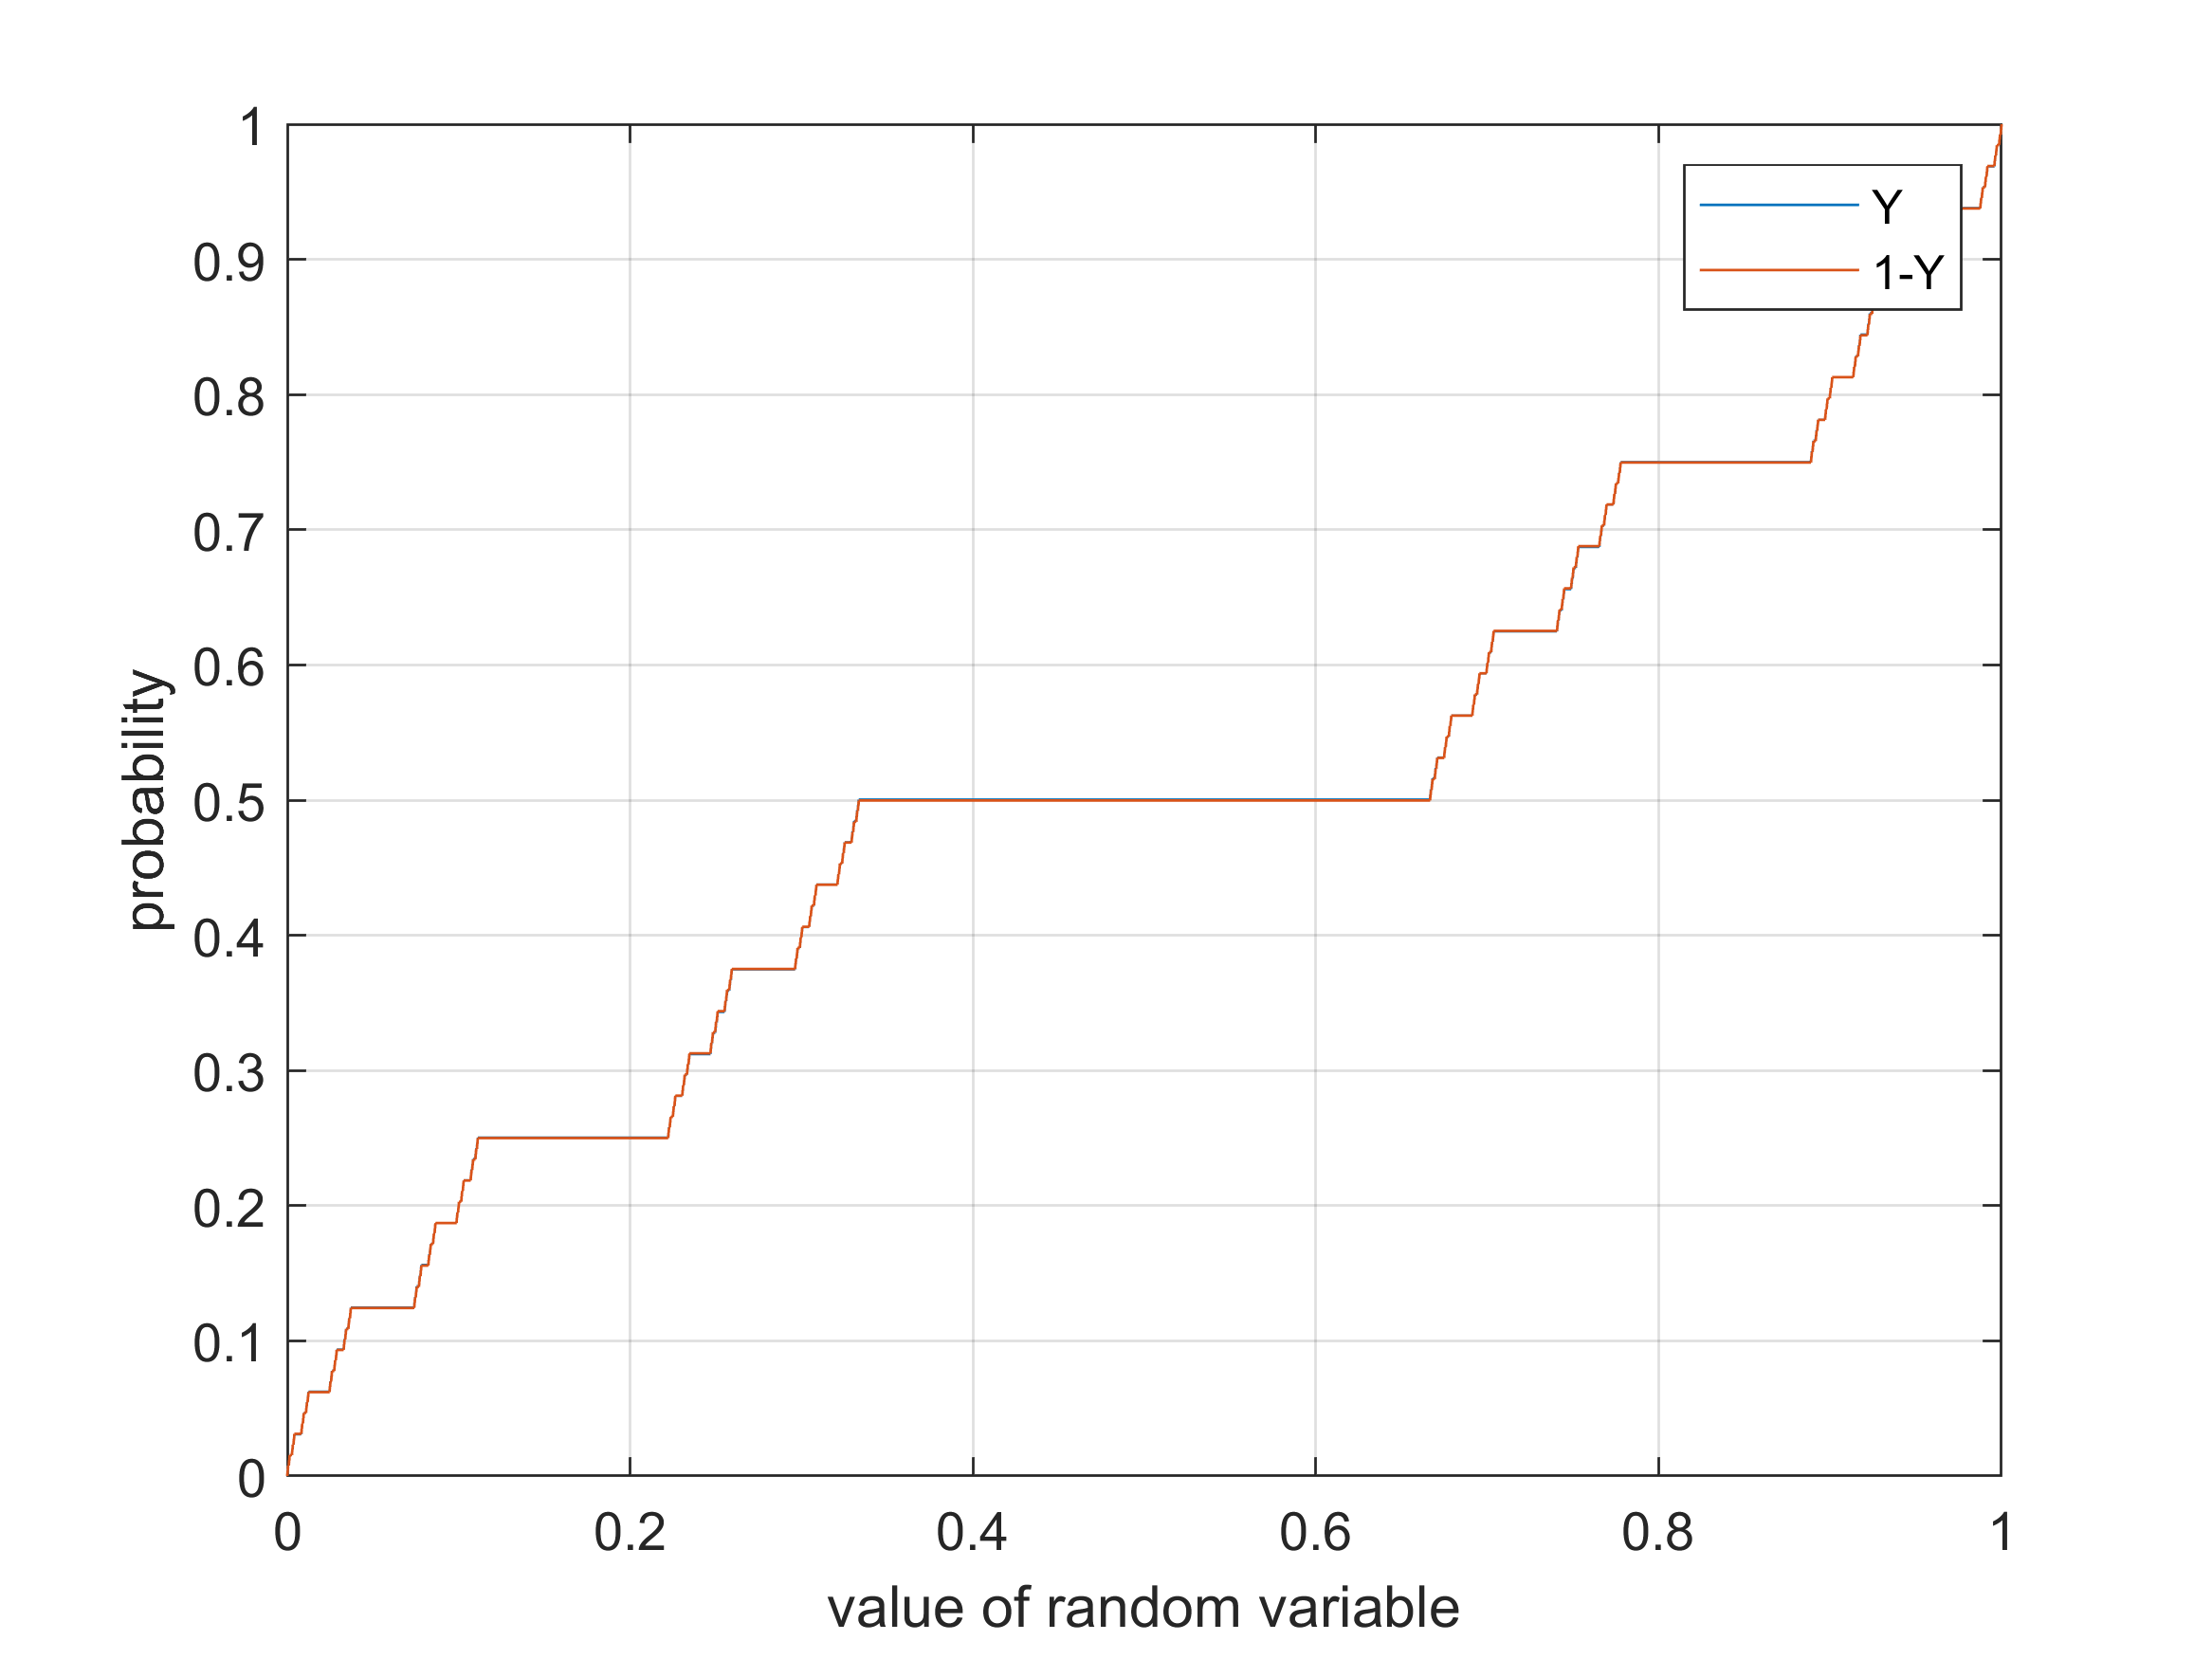
\includegraphics[width=0.6\textwidth]{../code/Task_2/pict/sim_1_vis_ex.png}
		\caption{Симметрия относительно 1/2 при $n=10^6$. }
    \end{figure}

	\begin{table}[h!]
	\begin{center}
		\begin{tabular}{|c|c|c|c|}
			\hline $N$ & частота принятия гипотезы \\ \hline
				$10^2$ & 0.9  \\ \hline
				$10^3$ & 0.902 \\ \hline
		\end{tabular}
		\caption{Результаты проверки симметричности относительно 1/2 при $n=10^6, \alpha = 0.05$.}
	\end{center}
	\end{table}
	\newpage
	Рассмотрим условное распределение $Y$ при условии, что $Y \in \left[0;\frac{1}{3}\right]$. Из построения 
	$Y$ видно, что $Y \in \left[0;\frac{1}{3}\right]$, если $\alpha_1 = 0$. Получаем:
	$$
		Y 	= \sum\limits_{k=2}^{\infty}\dfrac{2\alpha_k}{3^k} 
			= \sum\limits_{k=1}^{\infty}\dfrac{2\alpha_{k+1}}{3^{k+1}} 
			= \frac{1}{3}\sum\limits_{k=1}^{\infty}\dfrac{2\alpha_k}{3^k} 
			= \frac{1}{3}Y.
	$$
	
	\begin{table}[h!]
	\begin{center}
		\begin{tabular}{|c|c|c|c|}
			\hline $N$ & частота принятия гипотезы \\ \hline
				$10^2$ & 0.97  \\ \hline
				$10^3$ & 0.968 \\ \hline
		\end{tabular}
		\caption{Результаты проверки самоподобия относитеьно деления на 3 при $n=10^6, \alpha = 0.05$.}
	\end{center}
	\end{table}
	
	\begin{figure}[h!]
		\centering
		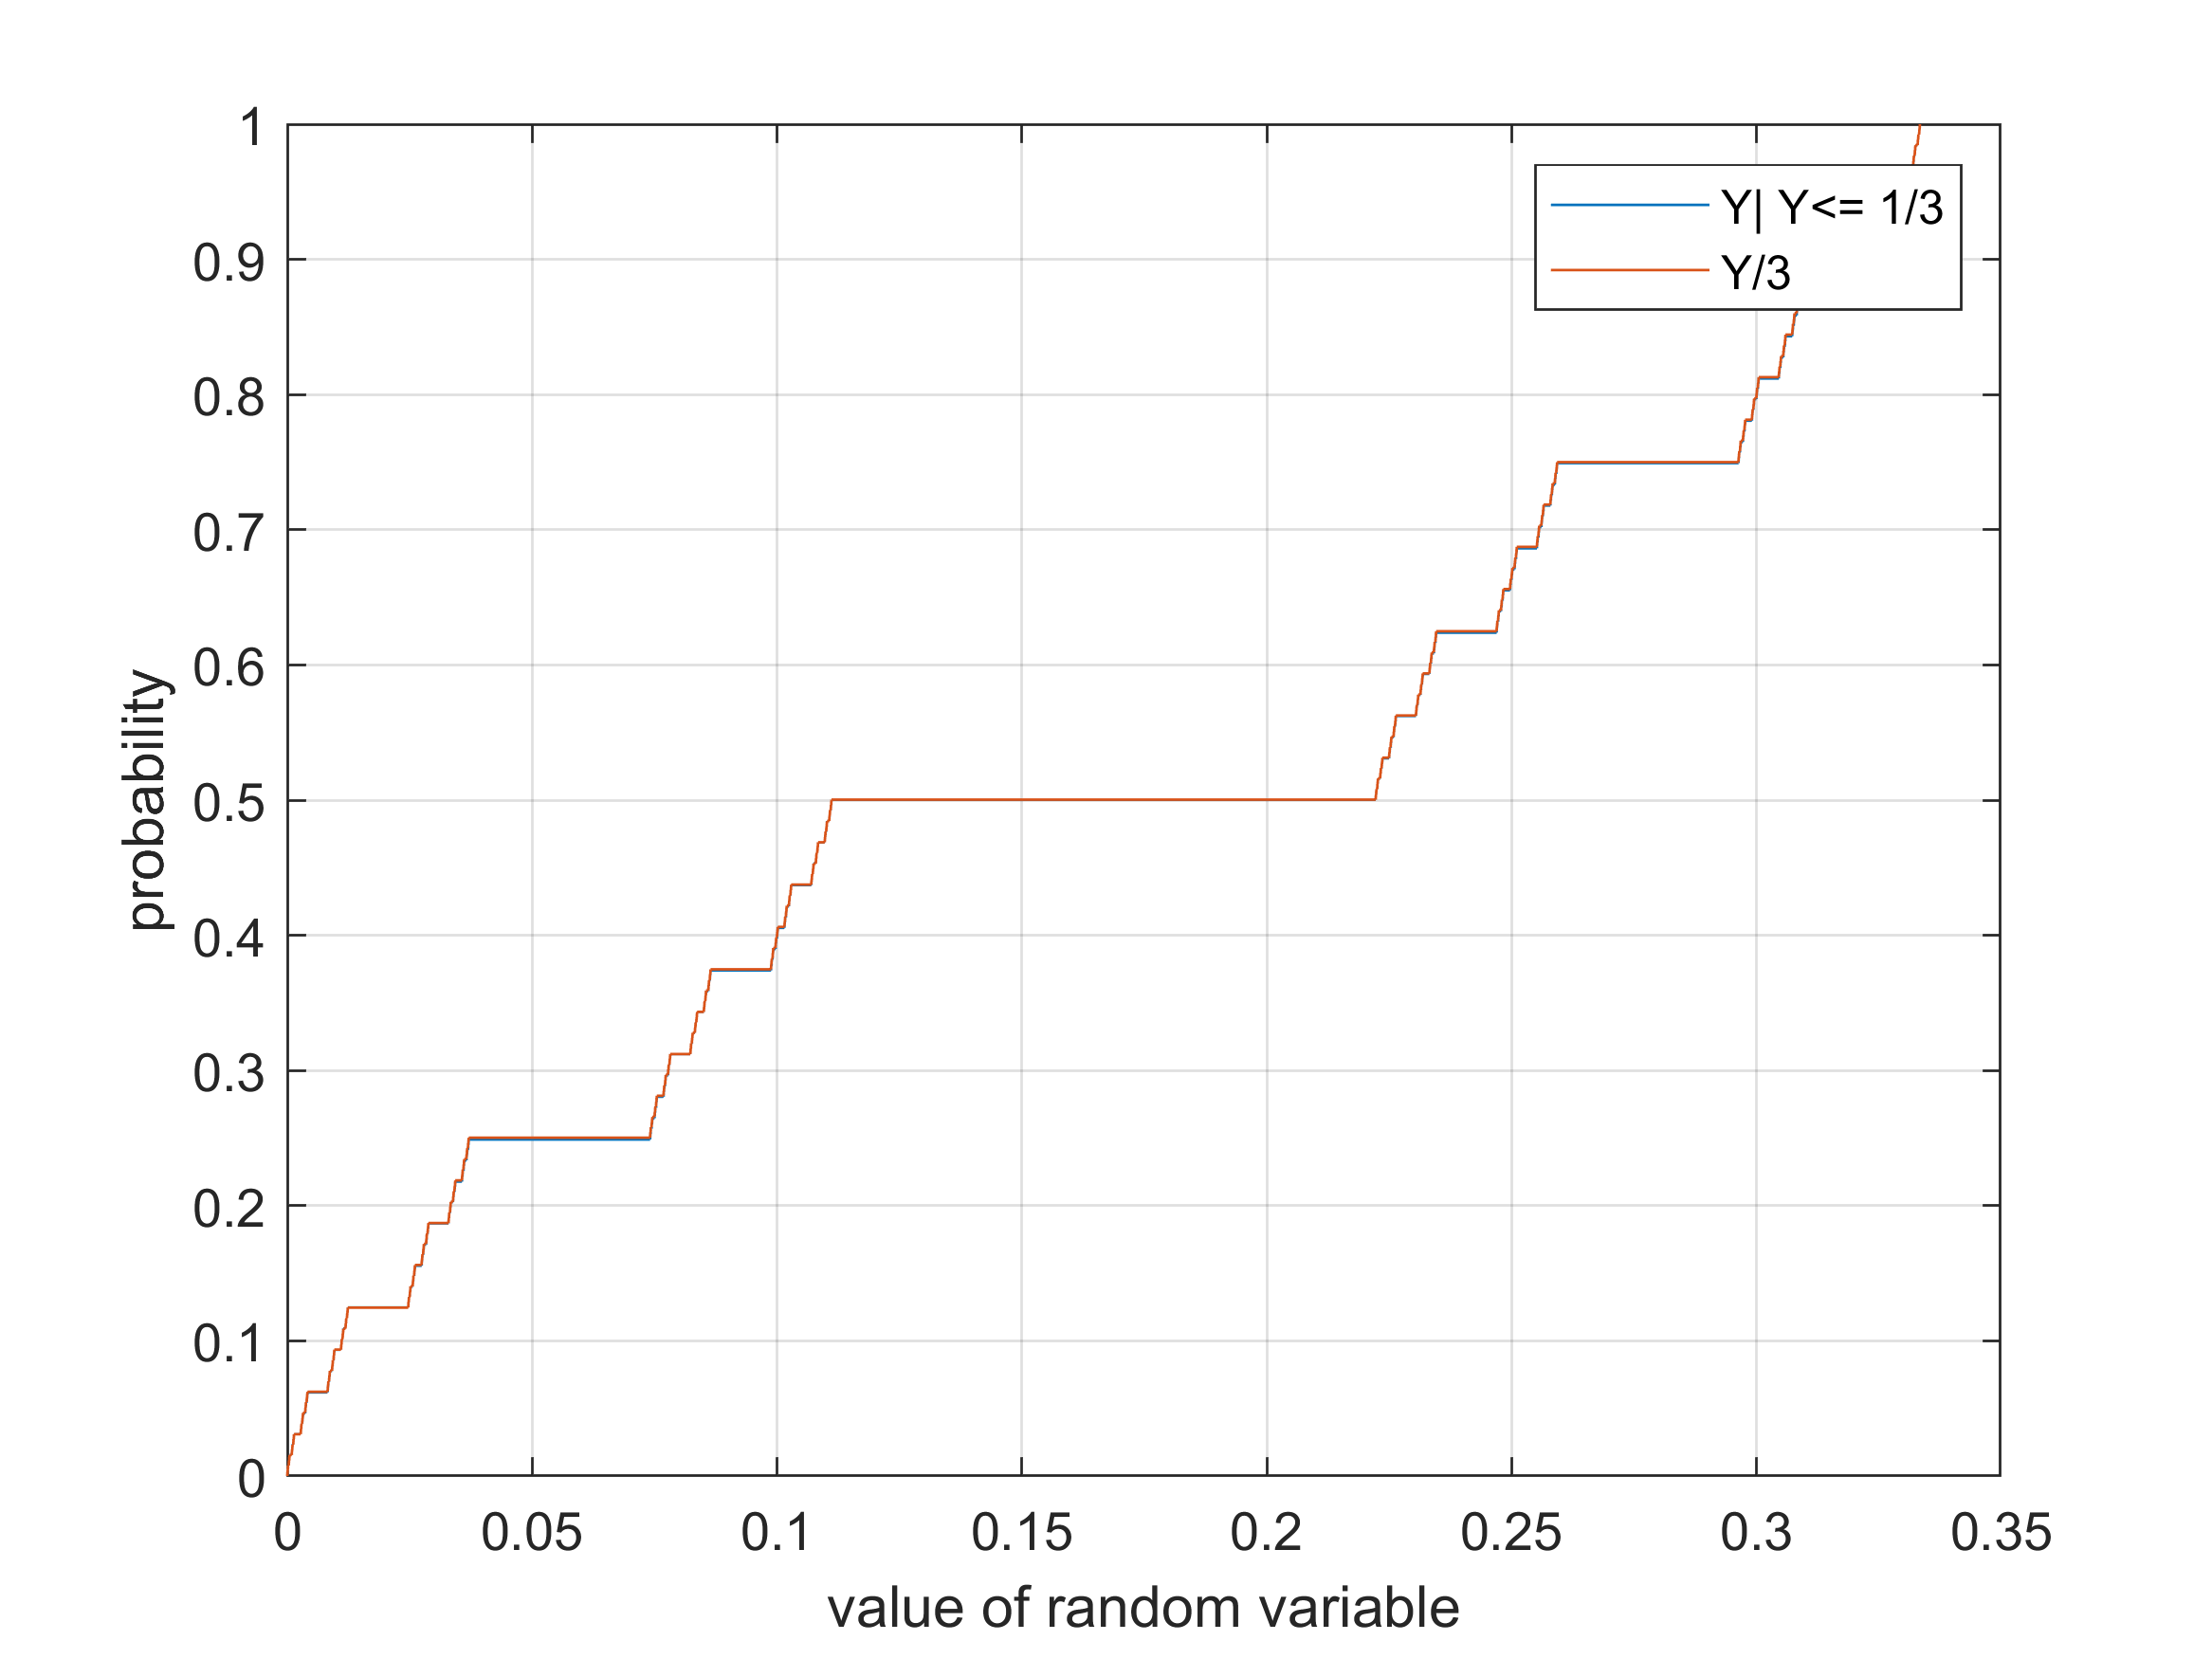
\includegraphics[width=0.6\textwidth]{../code/Task_2/pict/sim_2_vis_ex.png}
		\caption{Самоподобие относитеьно деления на 3 при $n=10^6$. }
    \end{figure}

\subsubsection{Пункт 3}
	Вычислим математическое ожидание и дисперсию для данного распределения:
	$$
		\begin{gathered}
			\E Y= \E \sum\limits_{k=1}^{\infty}\dfrac{2\alpha_k}{3^k}	
				  =  \sum\limits_{k=1}^{\infty}\dfrac{2}{3^k} \E \alpha_k 
				 =  \sum\limits_{k=1}^{\infty}\dfrac{2}{3^k} \dfrac{1}{2} = \dfrac{1}{2}, \\
			\Var Y = \Var \sum\limits_{k=1}^{\infty}\dfrac{2\alpha_k}{3^k}	
				  	  =  \sum\limits_{k=1}^{\infty}\left(\dfrac{2}{3^k}\right)^2 \Var \alpha_k 
				 	  =  \sum\limits_{k=1}^{\infty}\dfrac{4}{9^k} \dfrac{1}{4} = \dfrac{1}{8},
		\end{gathered}
	$$
	где $\alpha_k \sim Bern(0.5)$.
	\begin{figure}[h!]
		\centering
		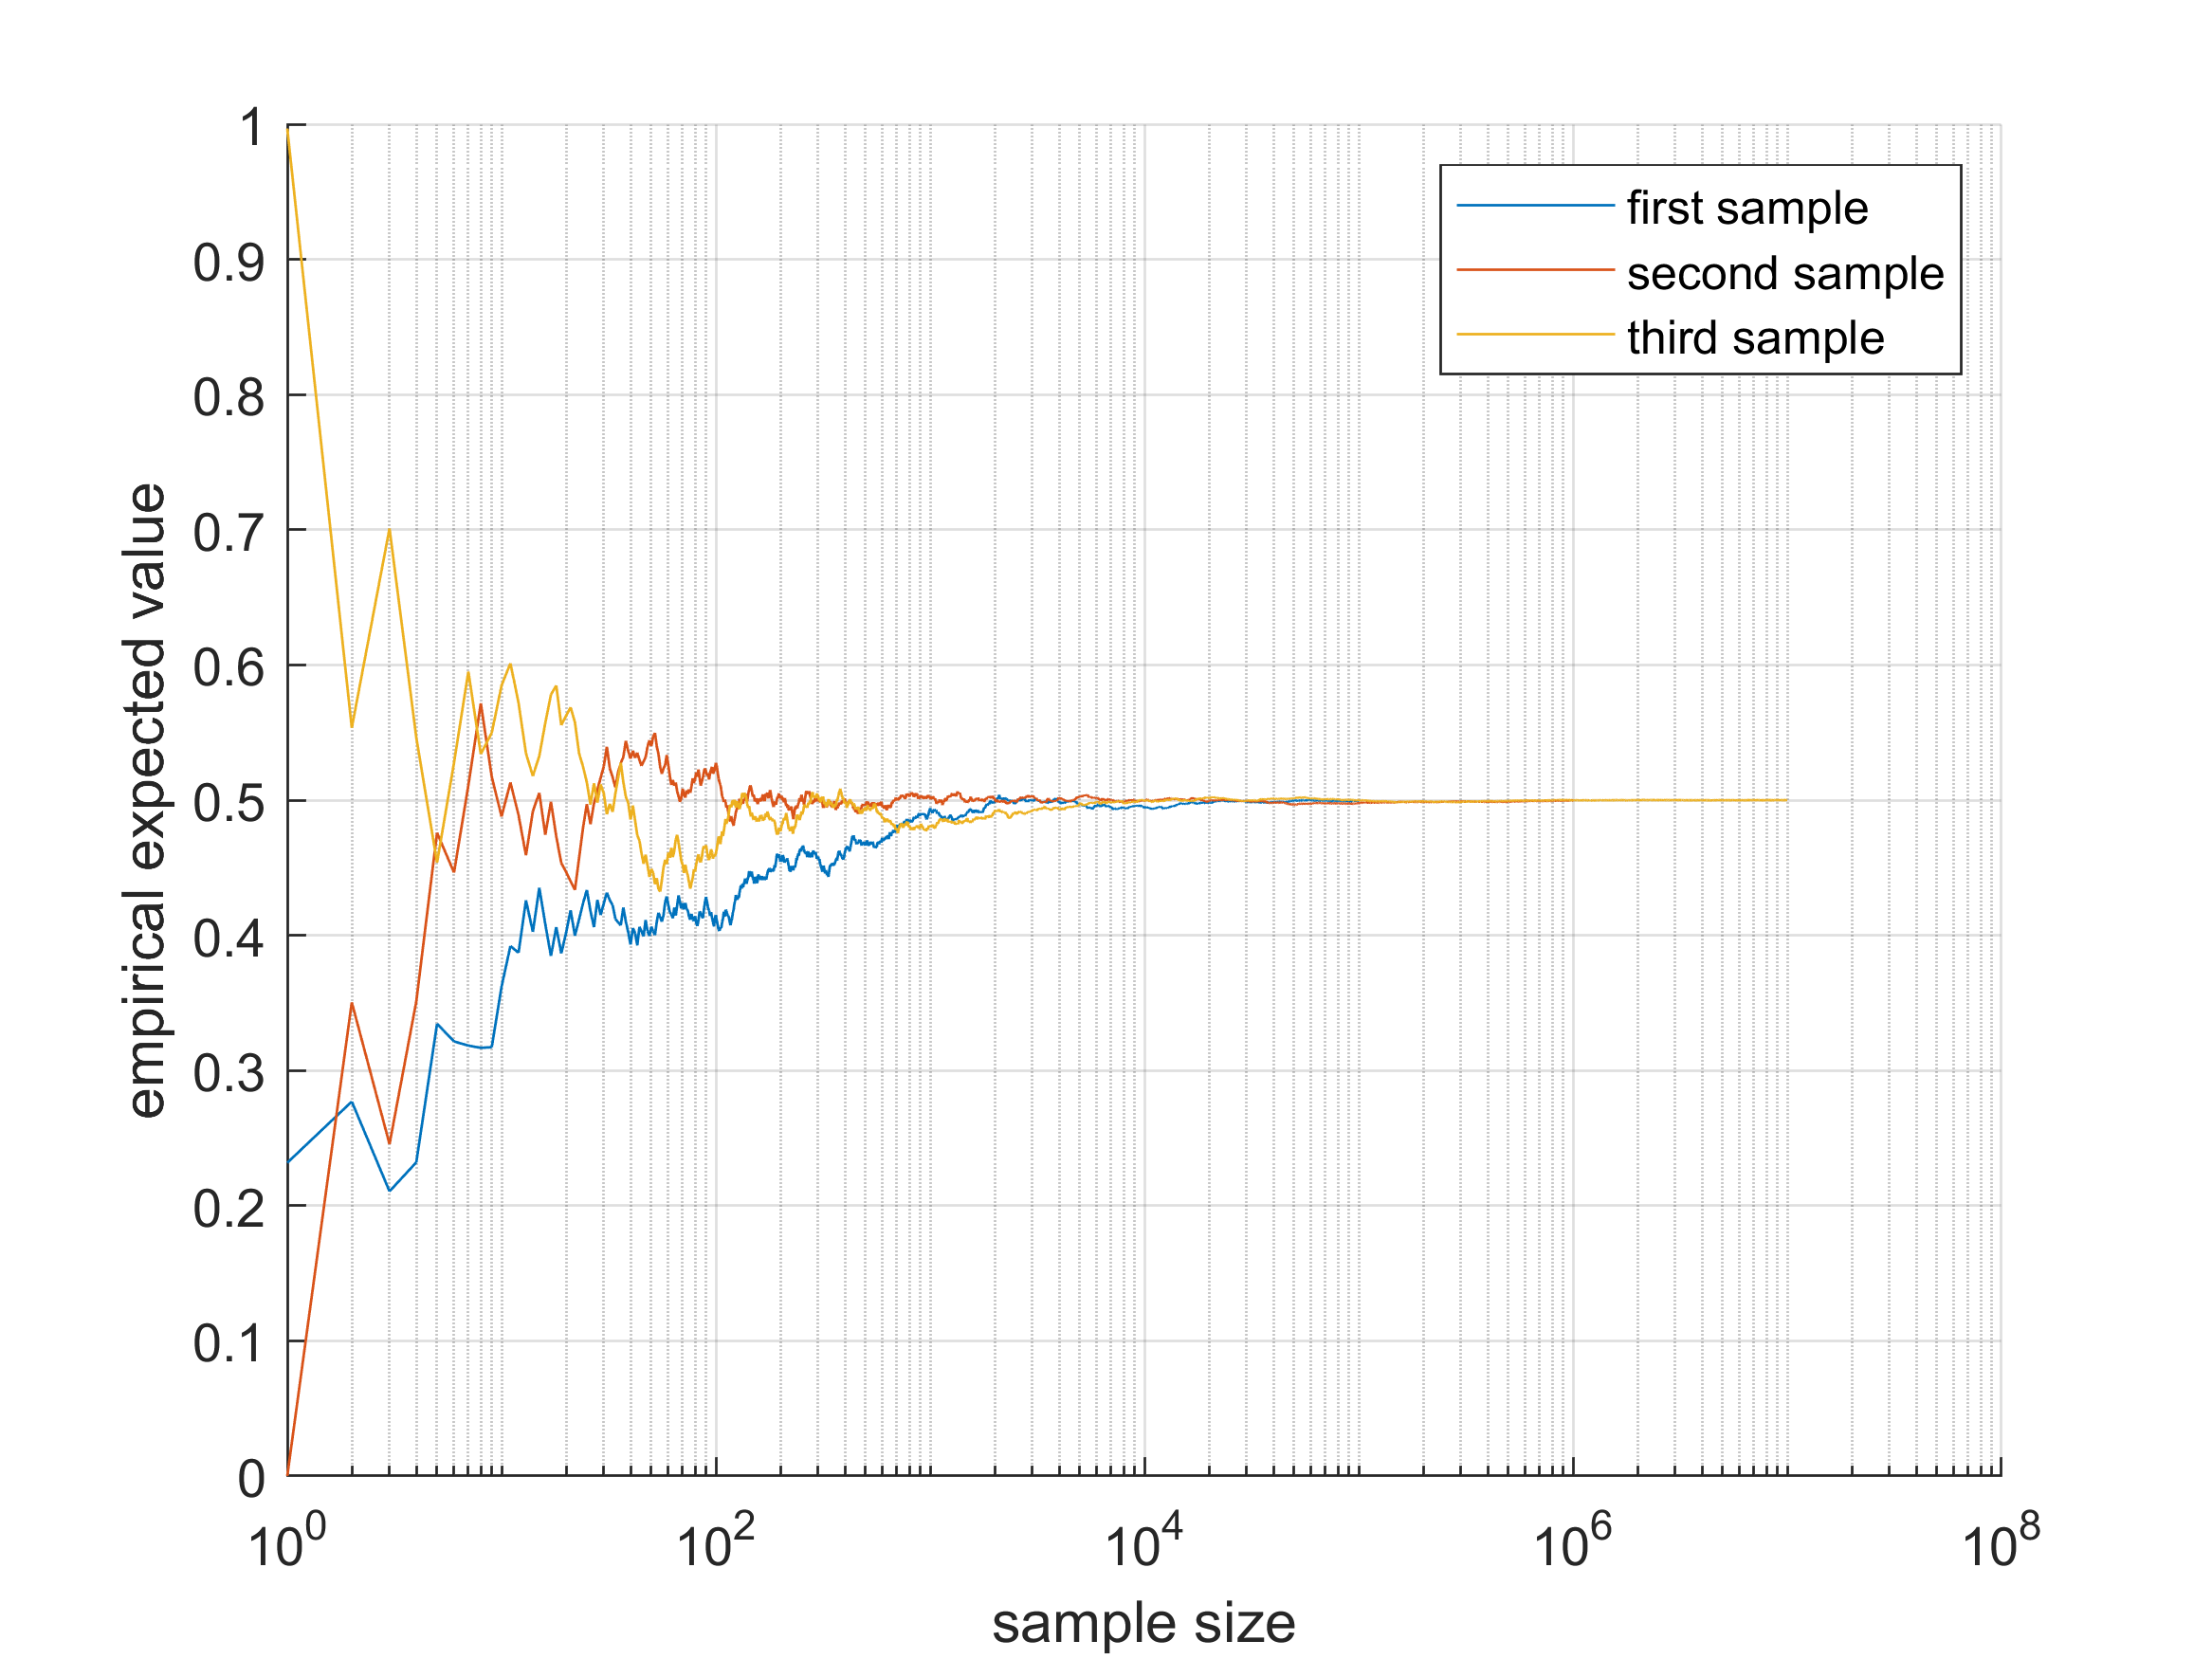
\includegraphics[width=0.6\textwidth]{../code/Task_2/pict/exp_val_vis_ex.png}
		\caption{Сходимость матожидания к 1/2 для нескольких выборок. }
    \end{figure}
	\newpage
	\begin{figure}[h!]
		\centering
		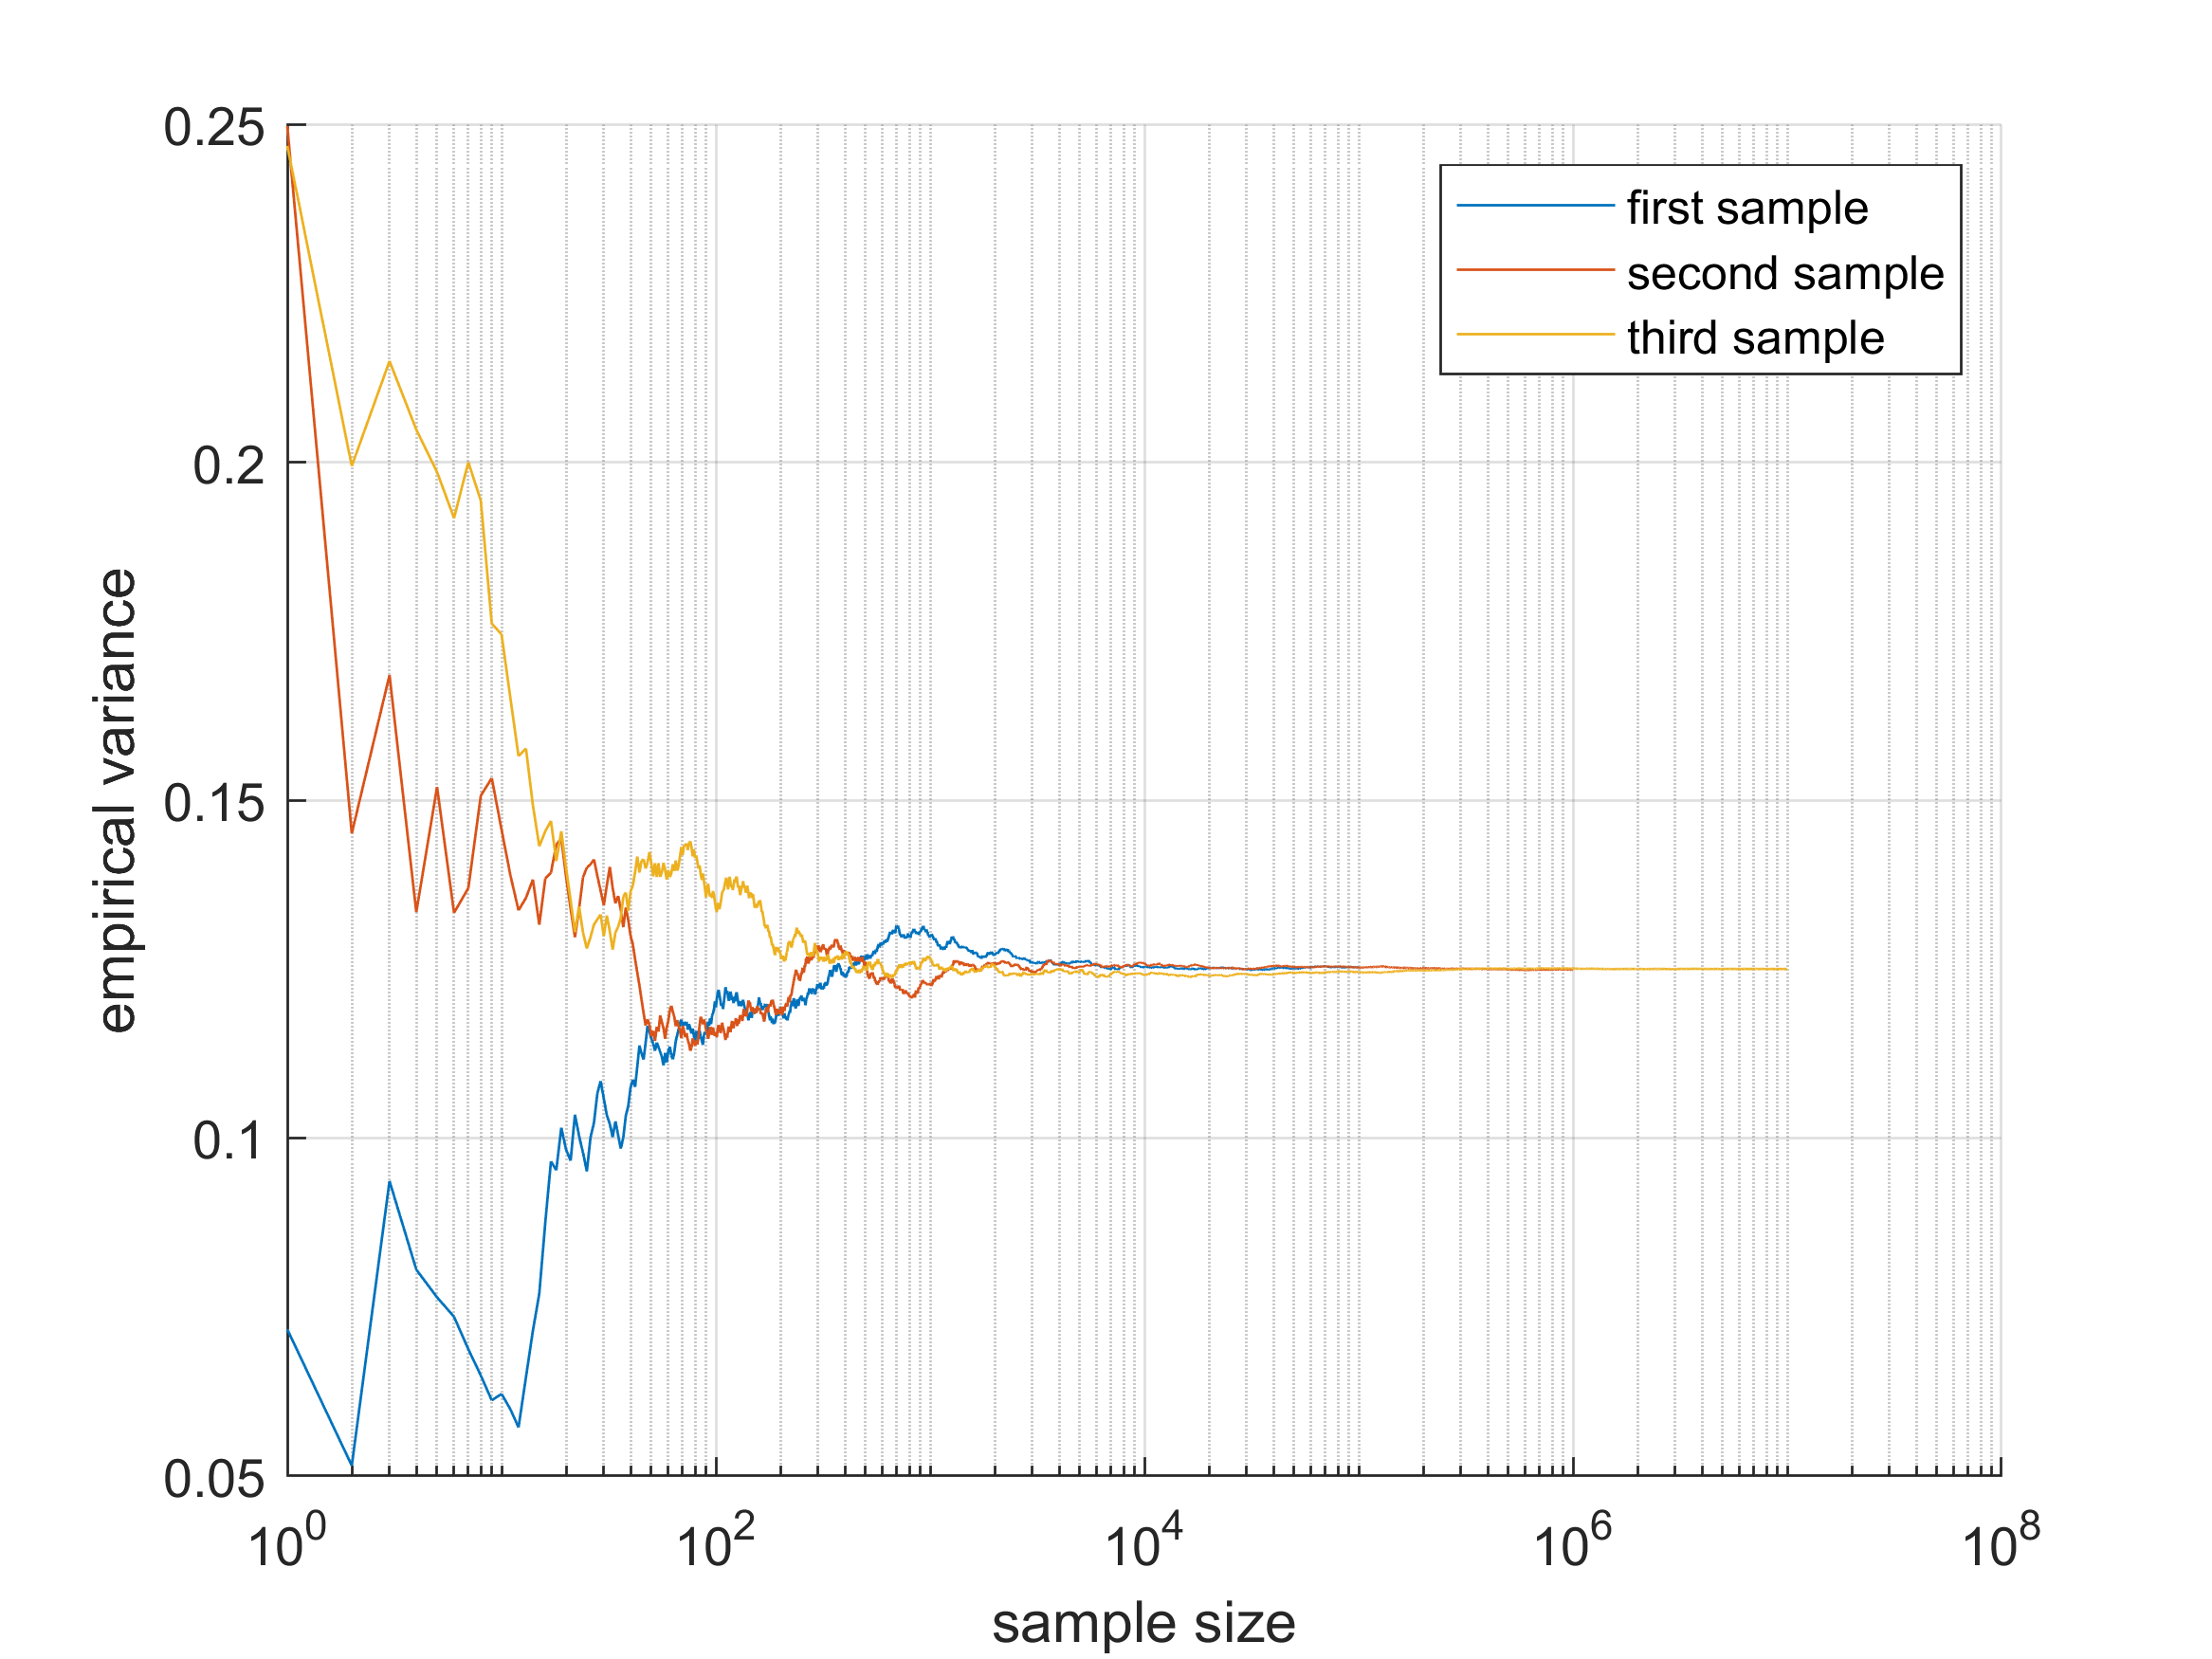
\includegraphics[width=0.6\textwidth]{../code/Task_2/pict/var_vis_ex.png}
		\caption{Сходимость дисперсии к 1/8 для нескольких выборок. }
    \end{figure}
	По иллюстрациям видно, что и математическое ожидание, и дисперсия сходятся
	к соответсвующим теоретически предсказанным величинам.

\newpage
\section{Задание 3}

\subsection{Постановка задачи}
    \begin{enumerate} 
        \item Построить датчик экспоненциального распределения. 
			Проверить для данного распределения свойство отсутствия памяти. Пусть 
        		$X_1, X_2, \ldots X_n$ -- независимо экспоненциально распределенные с.в. 
			с параметрами $\lambda_1, \lambda_2, \ldots \lambda_n$ соответственно.
			Найти распределение случайной величины $Y = \min{(X_1, X_2, \ldots X_n)}$.  
        \item На основе датчика экспоненциального распределения построить датчик
			пуассоновского распределения. 
        \item Построить датчик пуассоновского распределения как предел биномиального распределения.
			С помощью критерия хи- квадрат Пирсона убедиться, что получен датчик распределения Пуассона. 
        \item Построить датчик стандартного нормального распределения методом моделирования случайных
			величин парами с переходом в полярные координаты. Проверить при помощи
			критерия t- Стьюдента равенство математических ожиданий,
			а при помощи критерия Фишера равенство дисперсий. 
    \end{enumerate}
\subsection{Решение задачи}
\subsubsection{Пункт 1}

	\begin{definition}
		Случайная величина $\xi$ имеет экспоненциальное распределение
		с параметром $\lambda > 0$, если её функция распределения имеет вид:
		$$
			F_{\xi}(x) = \begin{cases}	
									1 - e^{-\lambda x}, & x\geqslant 0, \\
									0, & x<0
								\end{cases}
		$$
	\end{definition}
	
	\begin{theorem}
	 	Пусть функция $F(x)$ непрерывна и монотонно ворастает на $\mathbb{R}$, причем
		\newline $\lim\limits_{x\rightarrow - \infty}F(x) = 0, \lim\limits_{x\rightarrow + \infty}F(x) = 1$, 
		случайная велчина $Y\sim U[0;1]$ распределение, то случайная величина $X=F^{-1}(Y)$ имеет 
		функцию распределения $F_X(x) = F(x).$
	\end{theorem}
	Доказательство можно найти в $\cite{book_inv}$.
	\newline
	Применим эту теорему для моделирования датчика экспоненциального распределения на основе 
	датчика равномерного.
	$$
			F_{\xi}(x) = 1 -e^{\lambda x} \Rightarrow F^{-1}_{\xi}(x) = -\frac{1}{\lambda}\ln(1-x).
	$$ 
	Таким образом, если $Y\sim U[0;1],$ то
	$$
		X = -\frac{1}{\lambda}\ln(1-Y)
	$$
	имеет экспонециальное распределение с параметром $\lambda$.
	\begin{figure}[h!]
		\centering
		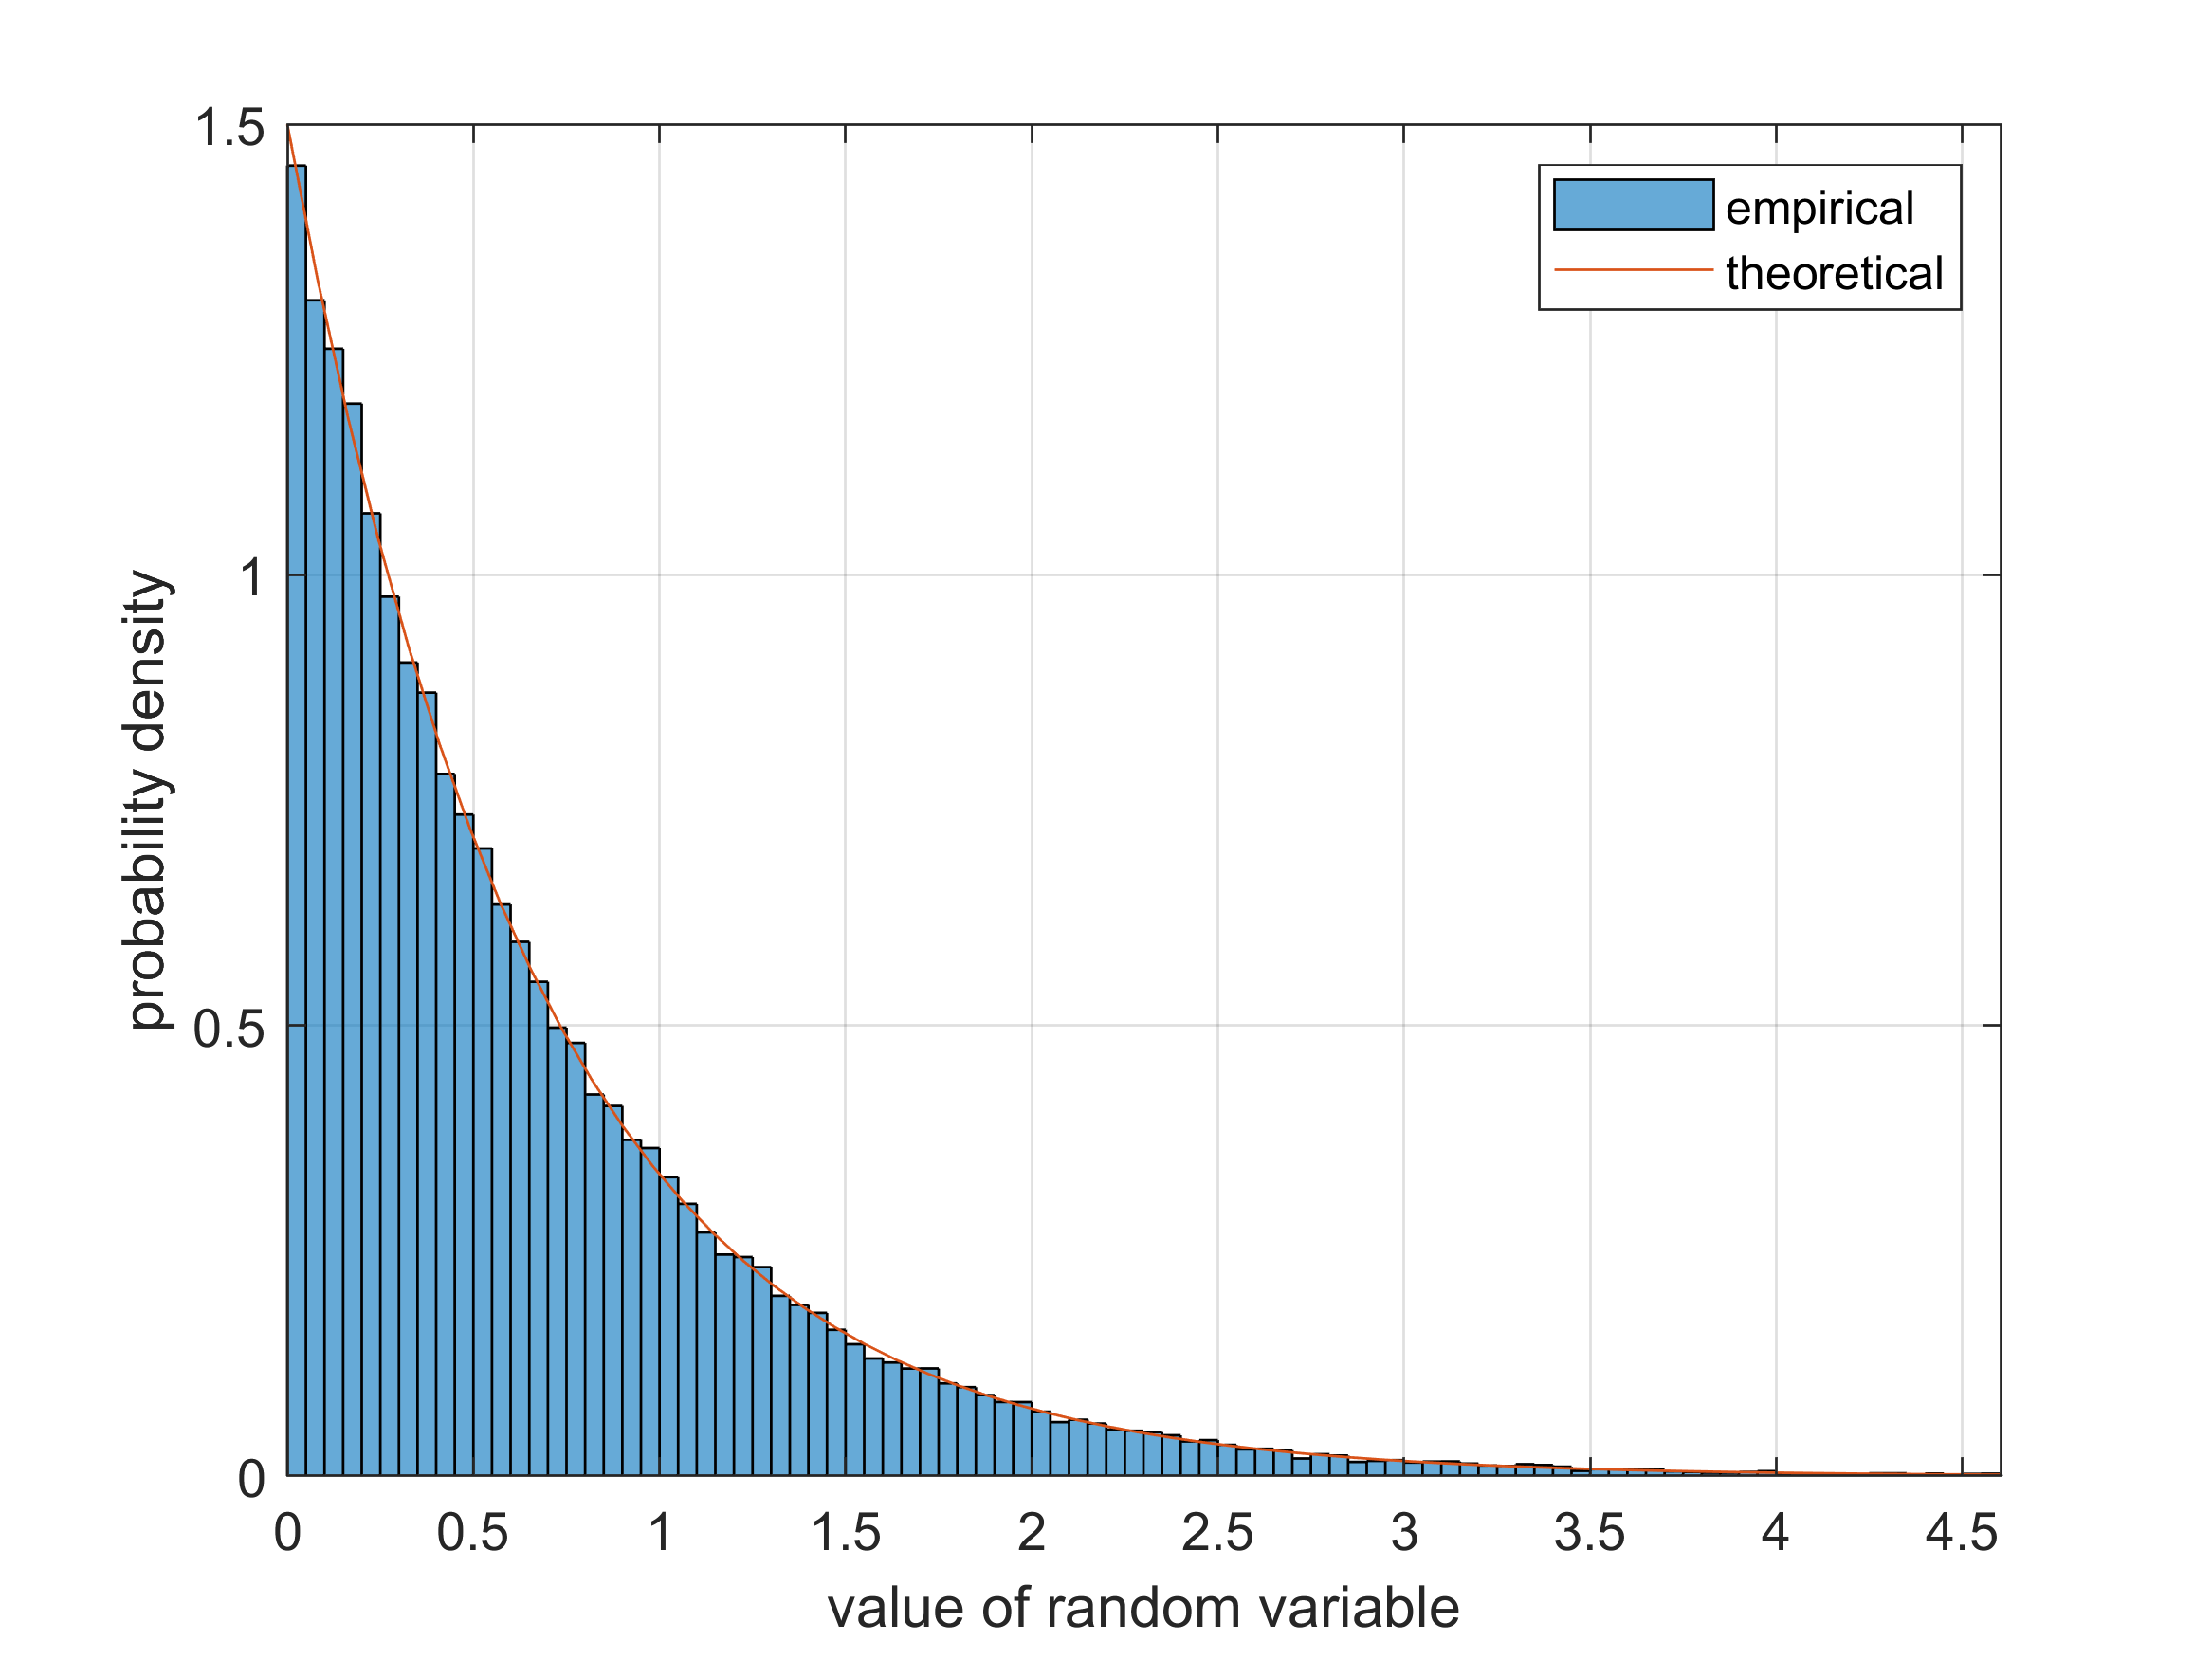
\includegraphics[width=0.6\textwidth]{../code/Task_3/pict/exp_vis_ex.png}
		\caption{Экспоненциальное распределение при $\lambda = 1.5$. }
    \end{figure}

    \begin{statement}
    Если $Z \sim Exp(\lambda)$, то выполняется 
            $$P(Z > t + s \mid Z > t) = P(Z > s)$$ для любых неотрицательных t и s. 
    \end{statement}

    \begin{proof}
        \begin{multline}
          \P(Z > t + s \mid Z > t) = \frac{\P(Z > t + s, Z > t)}{\P(Z > t)} = \frac{\P(Z > t+s)}{\P(Z > t)} 
					 = \frac{e^{-\lambda (t+s)}}{e^{-\lambda t}} = e^{-\lambda s} =\P(Y > n)
        \end{multline}
    \end{proof}
    Это называют свойством отсутствия памяти у экспоненциального распределения.
	
    \begin{figure}[h!]
		\centering
		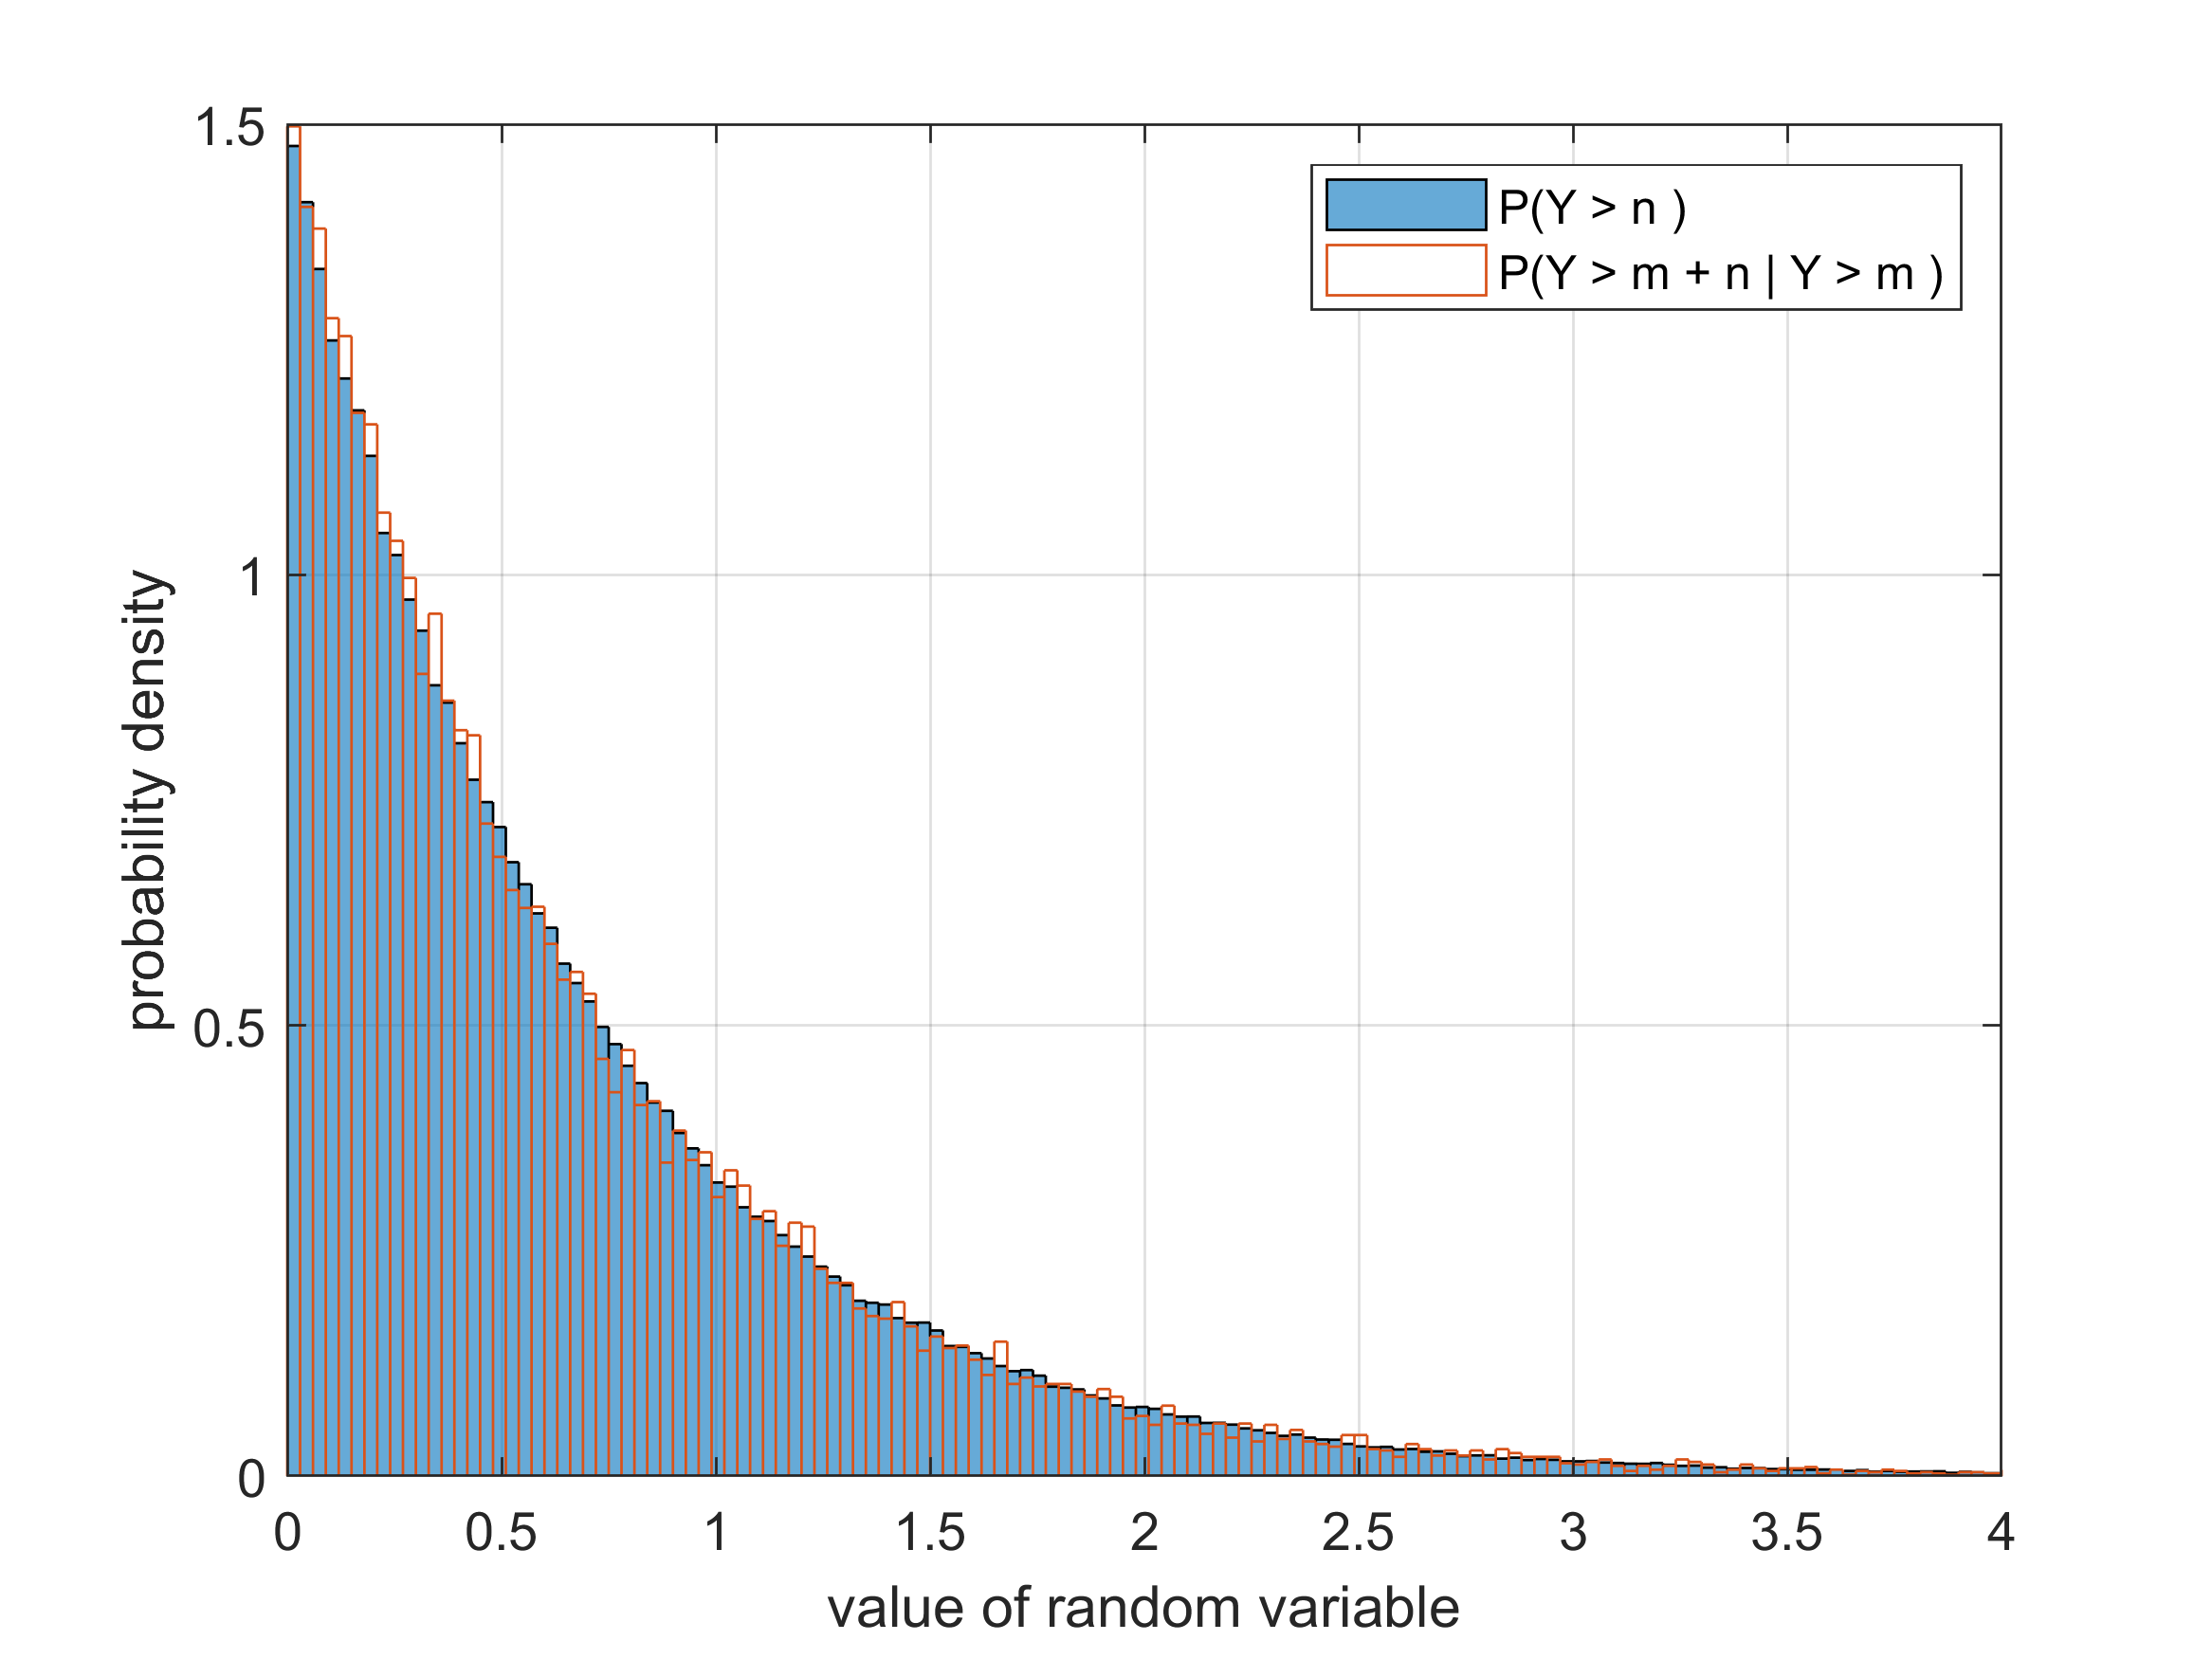
\includegraphics[width=0.6\textwidth]{../code/Task_3/pict/mmls_prop_ex.png}
		\caption{Свойство отсутствия памяти экспоненциального распределения. 
		\newline \centering  Параметры: $\lambda= 1.5, n=0.4, m=1.5$, размер выборки $10^6$.}
    \end{figure}

	\newpage
	\begin{statement}
	Пусть $X_1,X_2, \ldots, X_n$--- н.о.р.с.в.: $X_k \sim Exp(\lambda_k)$. \newline
	Тогда $Y=min(X_1, X_2, \ldots,X_n )\sim Exp(\lambda_0), \lambda_0 = \sum\limits_{k=1}^n{\lambda_k}.$
 	\end{statement}
	\begin{proof}
        \begin{multline}
          \P(\min(X_1,\ldots, X_n) >x) = \P(X_1> x, \ldots, X_n>x)= \prod\limits_{k=1}^n\P(X_k> x) = \\
					 =  \prod\limits_{k=1}^n \exp(-\lambda_k x)=  \exp(-x \sum\limits_{k=1}^n \lambda_k ).
        \end{multline}
    \end{proof}
	
 	\begin{figure}[h!]
		\centering
		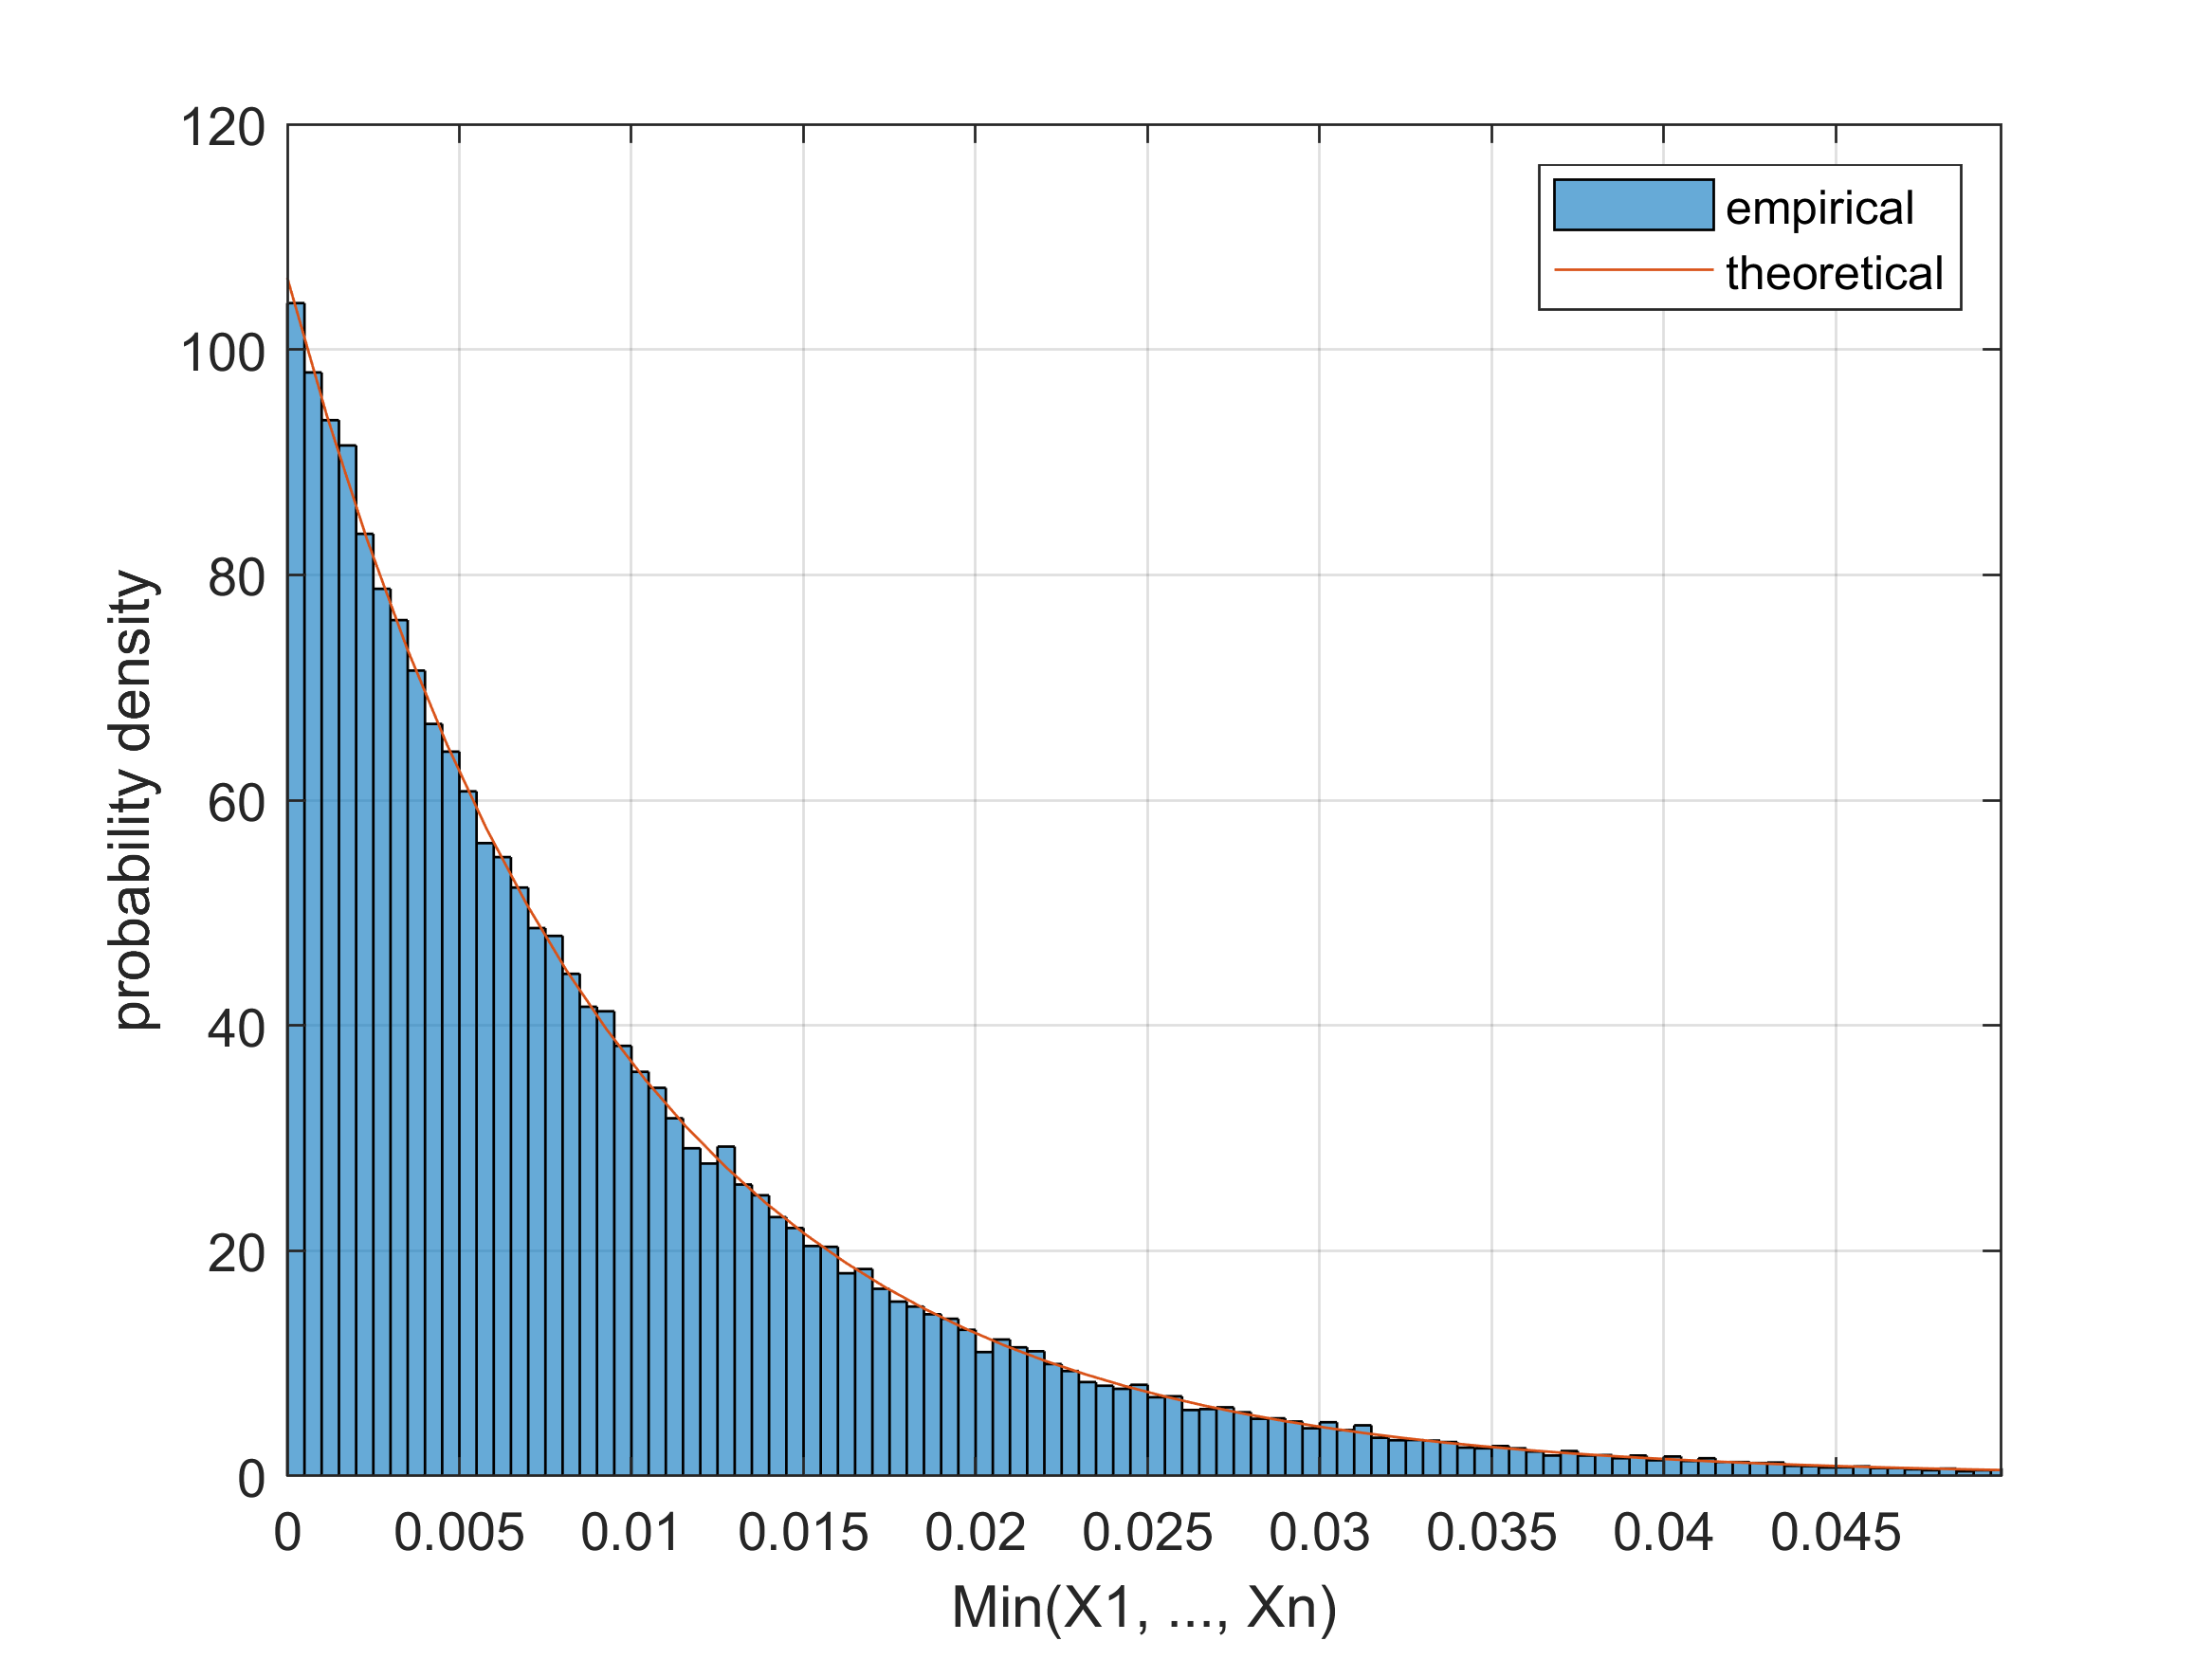
\includegraphics[width=0.6\textwidth]{../code/Task_3/pict/exp_min_ex.png}
		\caption{Распределение минимума из вектора экспоненциально распределенных с.в. 
		\newline \centering  для $N=10^4$ выборок. Параметры: $\lambda_0 \approx 106.4$, размер выборки $100$.}
    \end{figure}
	
\subsubsection{Пункт 2}
	\begin{definition}
		Случайная величина $X$ имеет распределение Пуассона с параметром $\lambda > 0$, если
		$$
			\P(X=k) = \frac{\lambda^k}{k!}e^{-\lambda}, \quad k \in \mathbb{N} \cup {0}.
		$$
	\end{definition}
	\begin{theorem}
		Пусть $X_1, X_2, \ldots, X_n, \ldots \sim Exp(\lambda)$ --- н.о.р.с.в. Тогда случайная величина 
		$$
			Y=\max\limits_n(S_n = X_1+X_2+\ldots+X_n)<1
		$$
		имеет распределение Пуассона с параметром $\lambda$. Если $X_1 \geqslant 1$, то $Y = 0.$
	\end{theorem}
	Доказательство этой теоремы можно найти в $\cite{feller}$.

	Таким образом, будем разыгрывать случайные величины $X_k\sim Exp(\lambda)$ до тех пор, пока их 
	сумма $S_n$ не превысит 1, и положим  $Y = n-1$.
	\begin{figure}[h!]
		\centering
		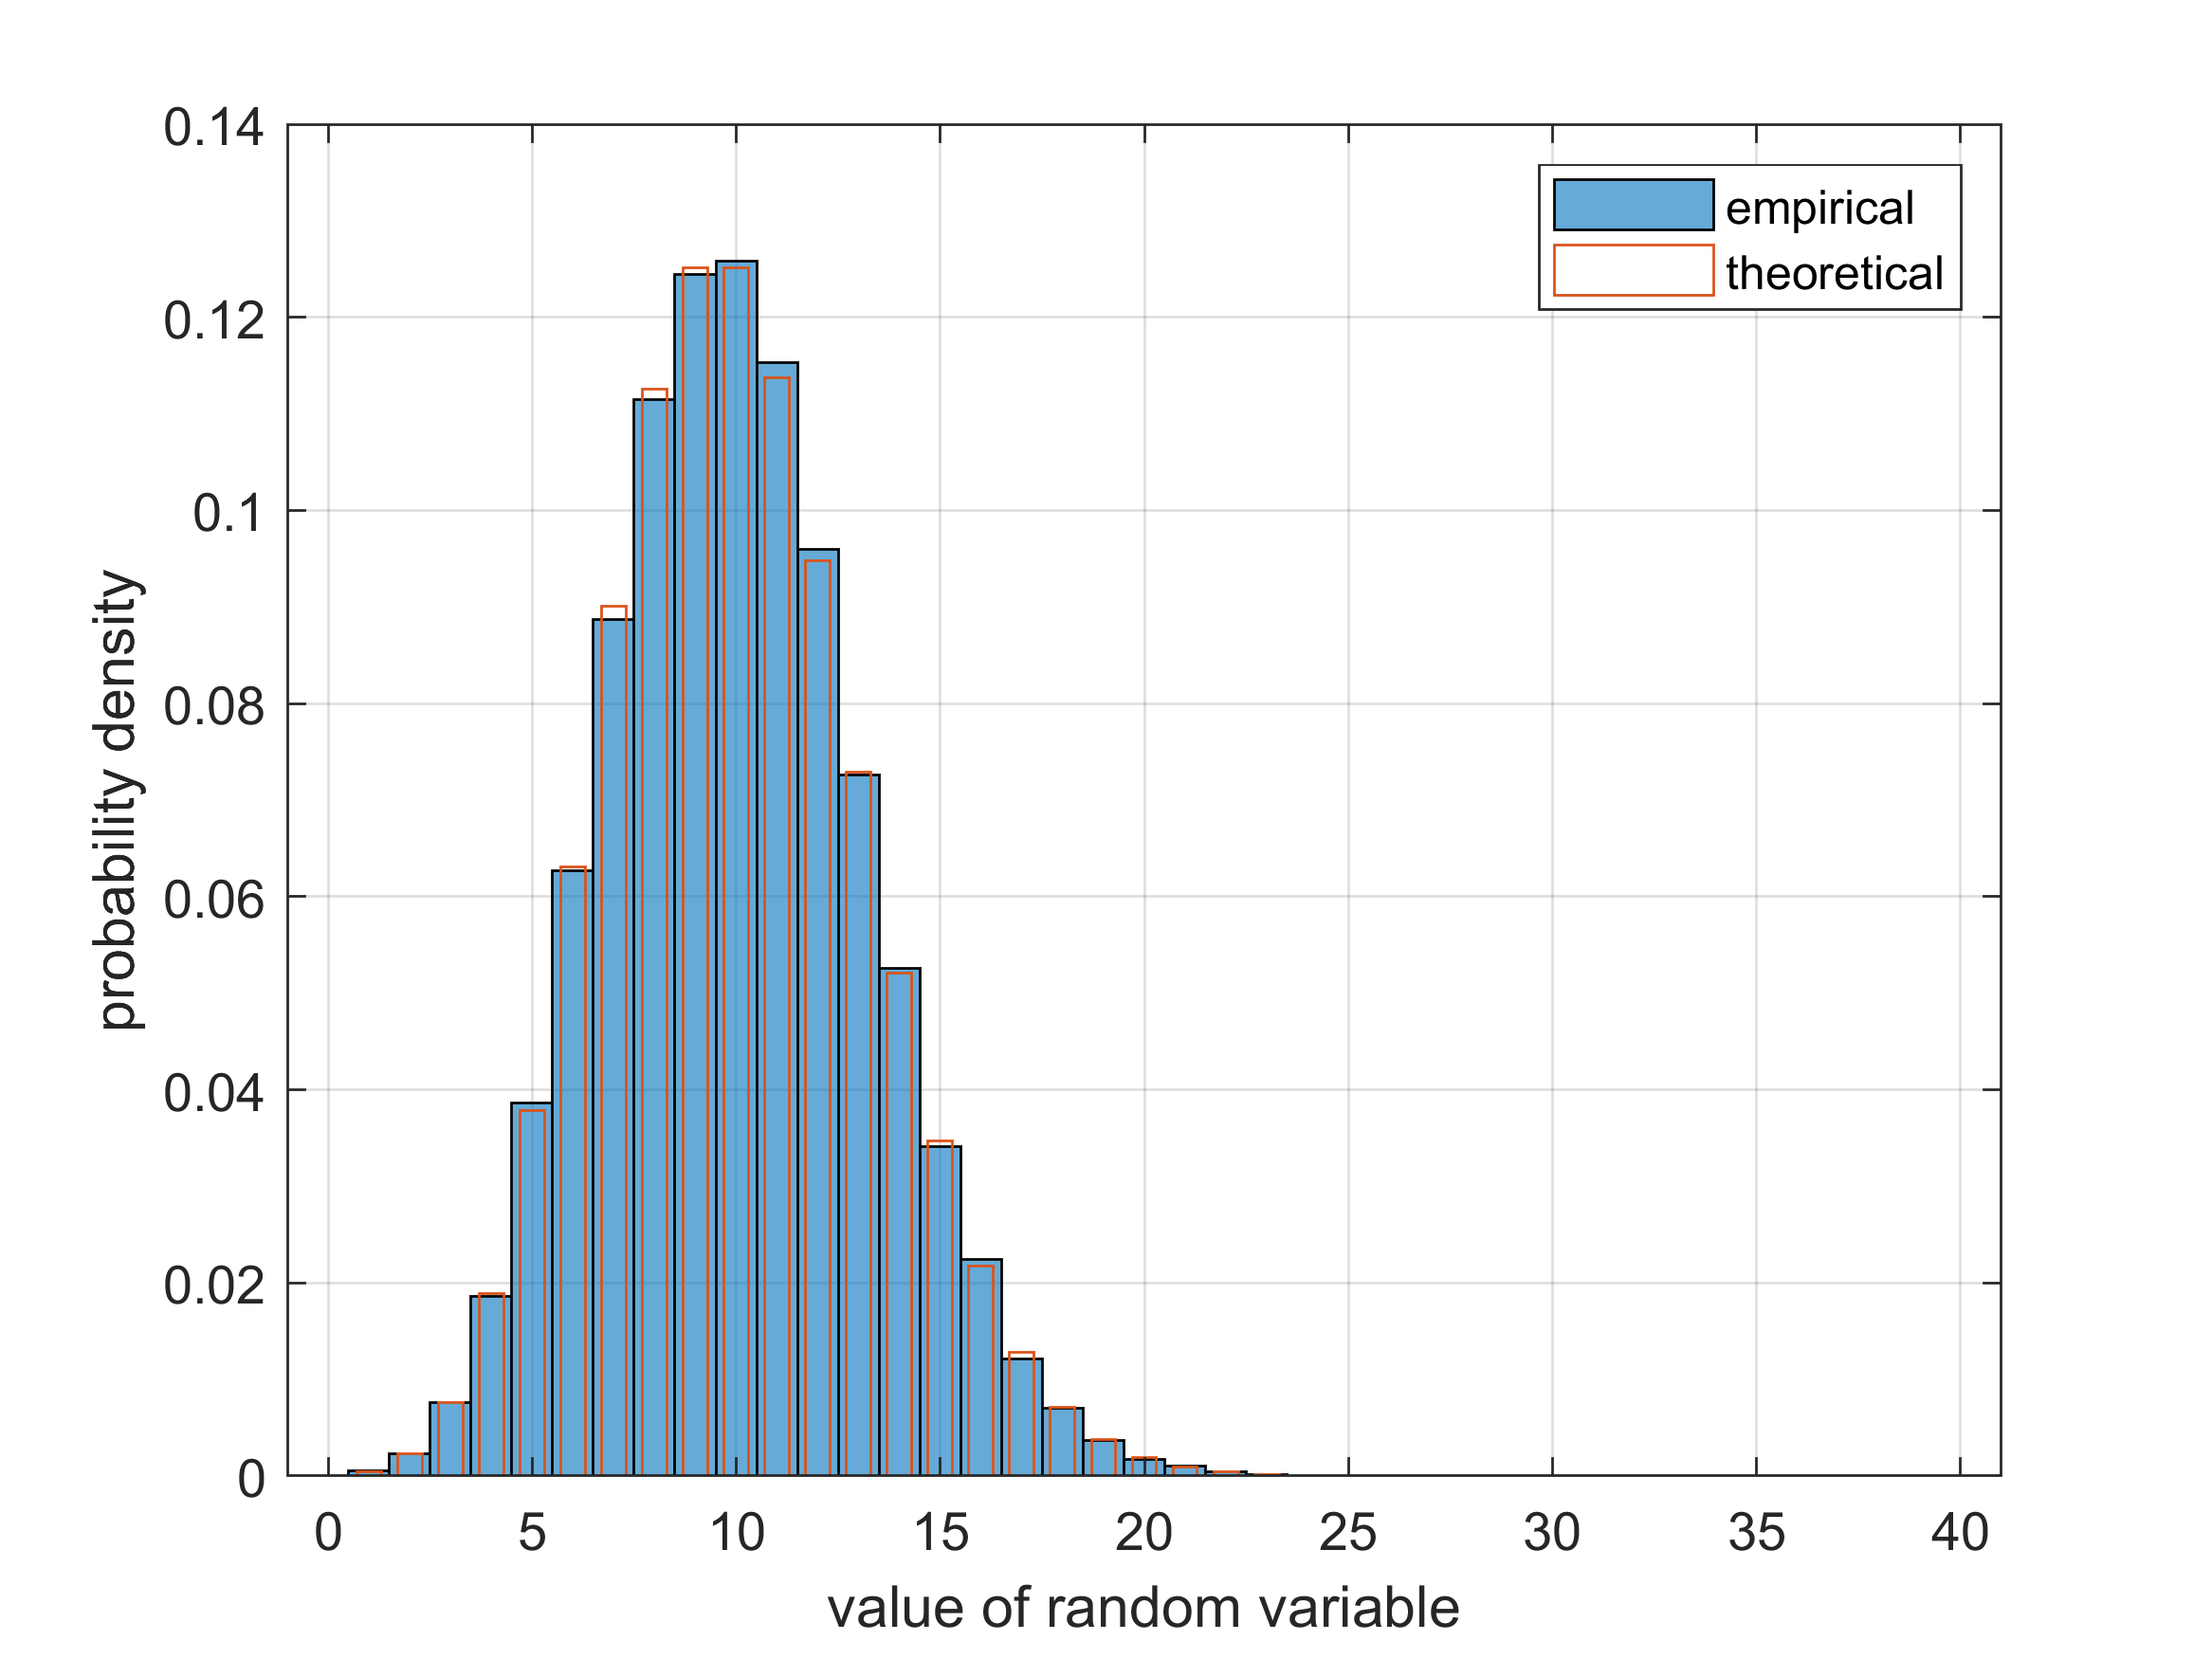
\includegraphics[width=0.6\textwidth]{../code/Task_3/pict/pois_exp_vis_ex.png}
		\caption{Распределение Пуассона, полученное на основе экспоненциального распределения. 
		\newline \centering Параметры: $\lambda = 10$, размер выборки $10^5$.}
    \end{figure}

\newpage
\subsubsection{Пункт 3}
	Другой способ моделирования пуассоновской случайной величины основывается на теореме Пуассона:
	\begin{theorem}
		Пусть случайная величина $X\sim Bi(n,p).$ Пусть $np=\lambda=$const.
		\newline Тогда при 
		$$
			\P (X=k) = C_n^kp^k(1-p)^{n-k} \xrightarrow{n \rightarrow \infty}
						 \dfrac{\lambda^k}{k!} e^{-\lambda}.
		$$
	\end{theorem}
	
	\begin{figure}[h!]
		\centering
		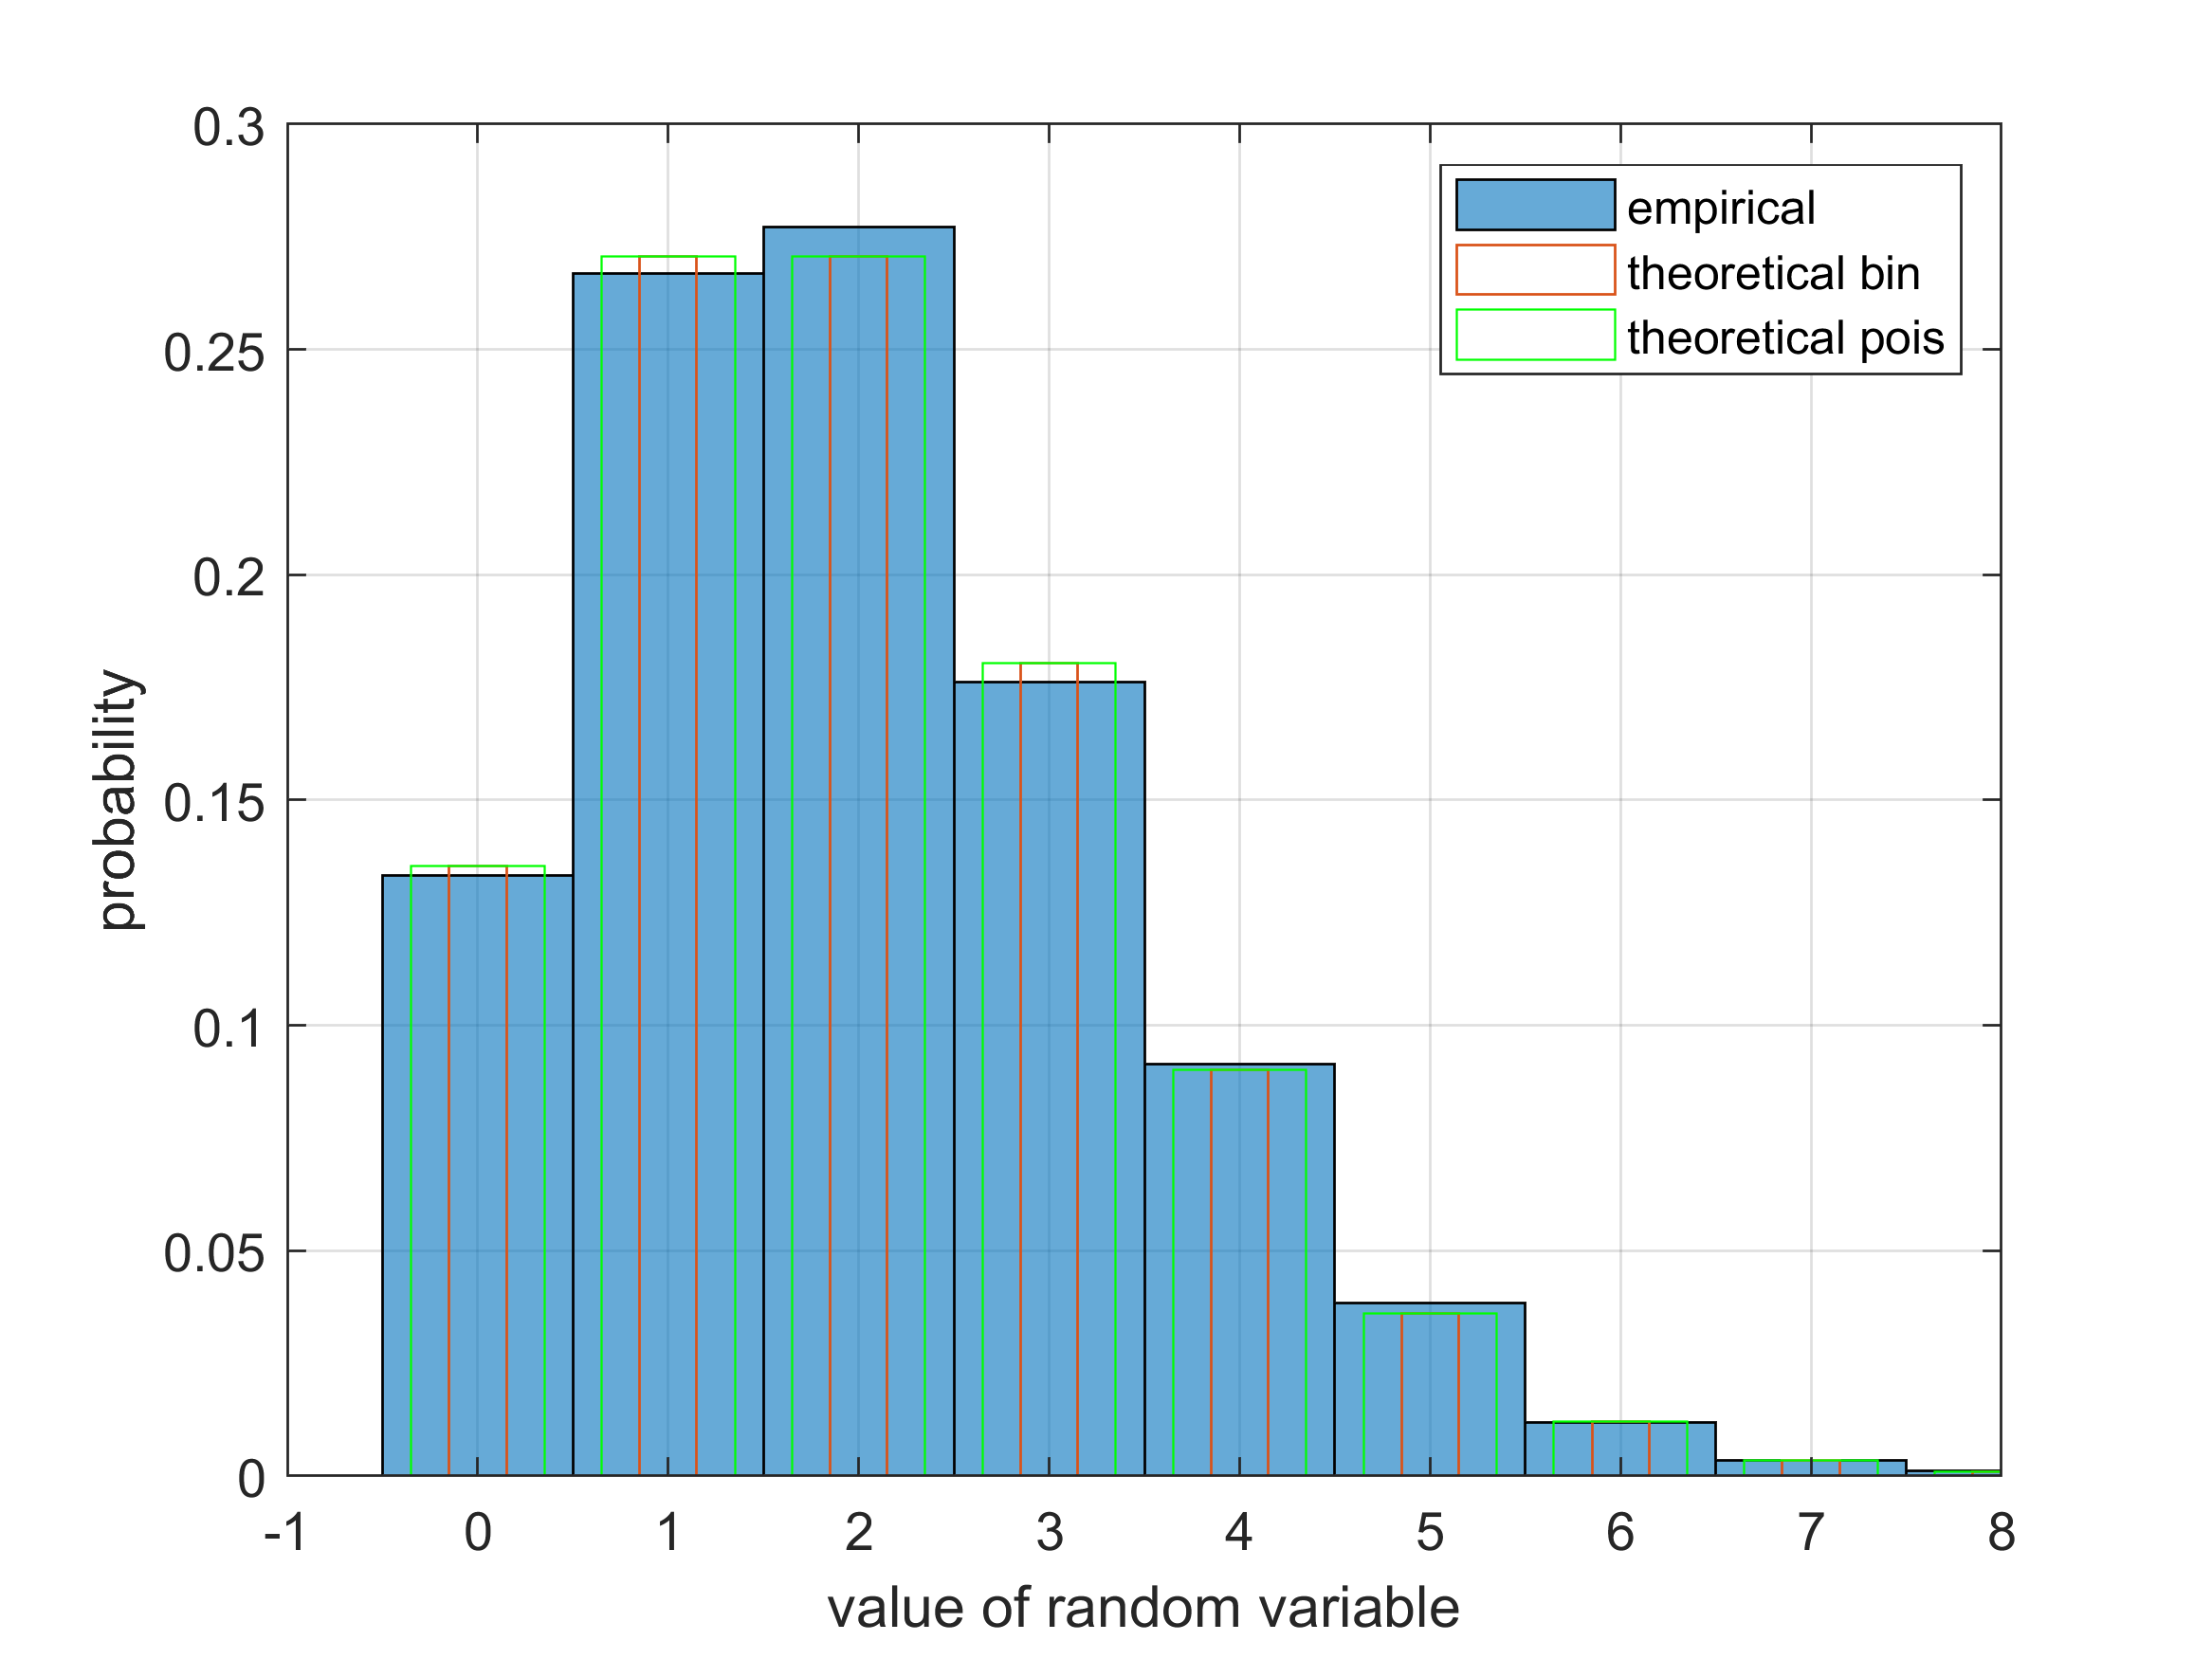
\includegraphics[width=0.6\textwidth]{../code/Task_3/pict/pois_bin_vis_ex.png}
		\caption{Распределение Пуассона как предел биномиального. 
		\newline \centering Параметры: $\lambda = 2$, размер выборки $10^4$.}
    \end{figure}

	Проверим результаты при помощи критерия Пирсона. \newline
	Исследуемое распределение принимает только целые неотрицательные значения.
	Обозначим за $n_i$ количество элементов в выборке равных $i$. Обозначим за $k$ 
	максимальное значение в выборке. Построим статистику критерия $X^2$ Пирсона:
	$$
		X^2_n =n \sum\limits_{i=1}^{k}\dfrac{\left(\dfrac{n_i}{n} - p_i\right)^2}{p_i},
	$$ 
	где $p_i=\P(Z=i), Z\sim Pois(\lambda)$.
	
	Гипотеза о пуассоновском распределении построенной выборки принимается на уровне значимости 
	$\alpha$, если вычисленное значение статистики $X_n^2$ не превосходит квантиль $\chi^2_{1-\alpha, r}$
	распределения $\chi_r^2$, где $r= k-1$.

	\begin{table}[h!]
	\begin{center}
		\begin{tabular}{|c|c|c|c|}
			\hline $N$ & частота принятия гипотезы \\ \hline
				$10^2$ & 0.92  \\ \hline
				$10^3$ & 0.894 \\ \hline
		\end{tabular}
		\caption{Проверка генерируемого распределения Пуассона как предела биномиального
						\newline \centering при $n=10^3$, размер выборки $10^4$ и уровне значимости $\alpha=0.05.$}
	\end{center}
	\end{table}

\subsubsection{Пункт 4}
	Для моделирования стандартного нормального распределения рассмотрим случаную величину
	$X=\{X_1, X_2\}\sim N(0,1):$
	$$
		\begin{gathered}
			\P(X_1<x_1, X_2<x_2) = \dfrac{1}{2\pi} \int\limits_{-\infty}^{x_1} \int\limits_{-\infty}^{x_2} 
														e^{-\dfrac{\xi^2+\eta^2}{2}}d\xi d\eta
			= \begin{Bmatrix}
					\xi = \rho \cos \phi, \\
					\eta = \rho \sin \phi, \\
					J = \rho
				\end{Bmatrix} = \\
			=	\dfrac{1}{2\pi} \iint\limits_{\begin{matrix} \rho \cos \phi < x_1 \\ \rho \sin \phi < x_2  \end{matrix}}	
						e^{-\dfrac{\rho^2}{2}}d\rho d\phi =  \begin{Bmatrix} \omega= \rho^2 \end{Bmatrix} 
			= \dfrac{1}{2\pi} \iint\limits_{\begin{matrix} \sqrt{\omega} \cos \phi < x_1 \\
																				 \sqrt{\omega} \sin \phi < x_2  
														  \end{matrix}}	
						\dfrac{1}{2}e^{-\dfrac{\omega}{2}}d\omega d\phi.
		\end{gathered}
	$$
	Подынтегральное выражение является произведением плотностей случайных величин 
	$Y_1\sim Exp(\frac{1}{2})$ и $Y_2\sim U[0;2\pi]$. Таким образом, совместное распределение
	случайных величин $X_1$ и $X_2$ совпадает с совместным распределением 
	$$
		\{\sqrt{Y_1}\cos Y_2, \sqrt{Y_1}\sin{Y_2}\}, \quad Y_1\sim Exp(\frac{1}{2}), \quad Y_2\sim U[0;2\pi].
	$$
	Заметим, что случайные величины $X_1$ и $X_2$ являются независимыми, так как их совместное
	распределение равно произведению их маргинальных распределений.
	
	\begin{figure}[h!]
		\centering
		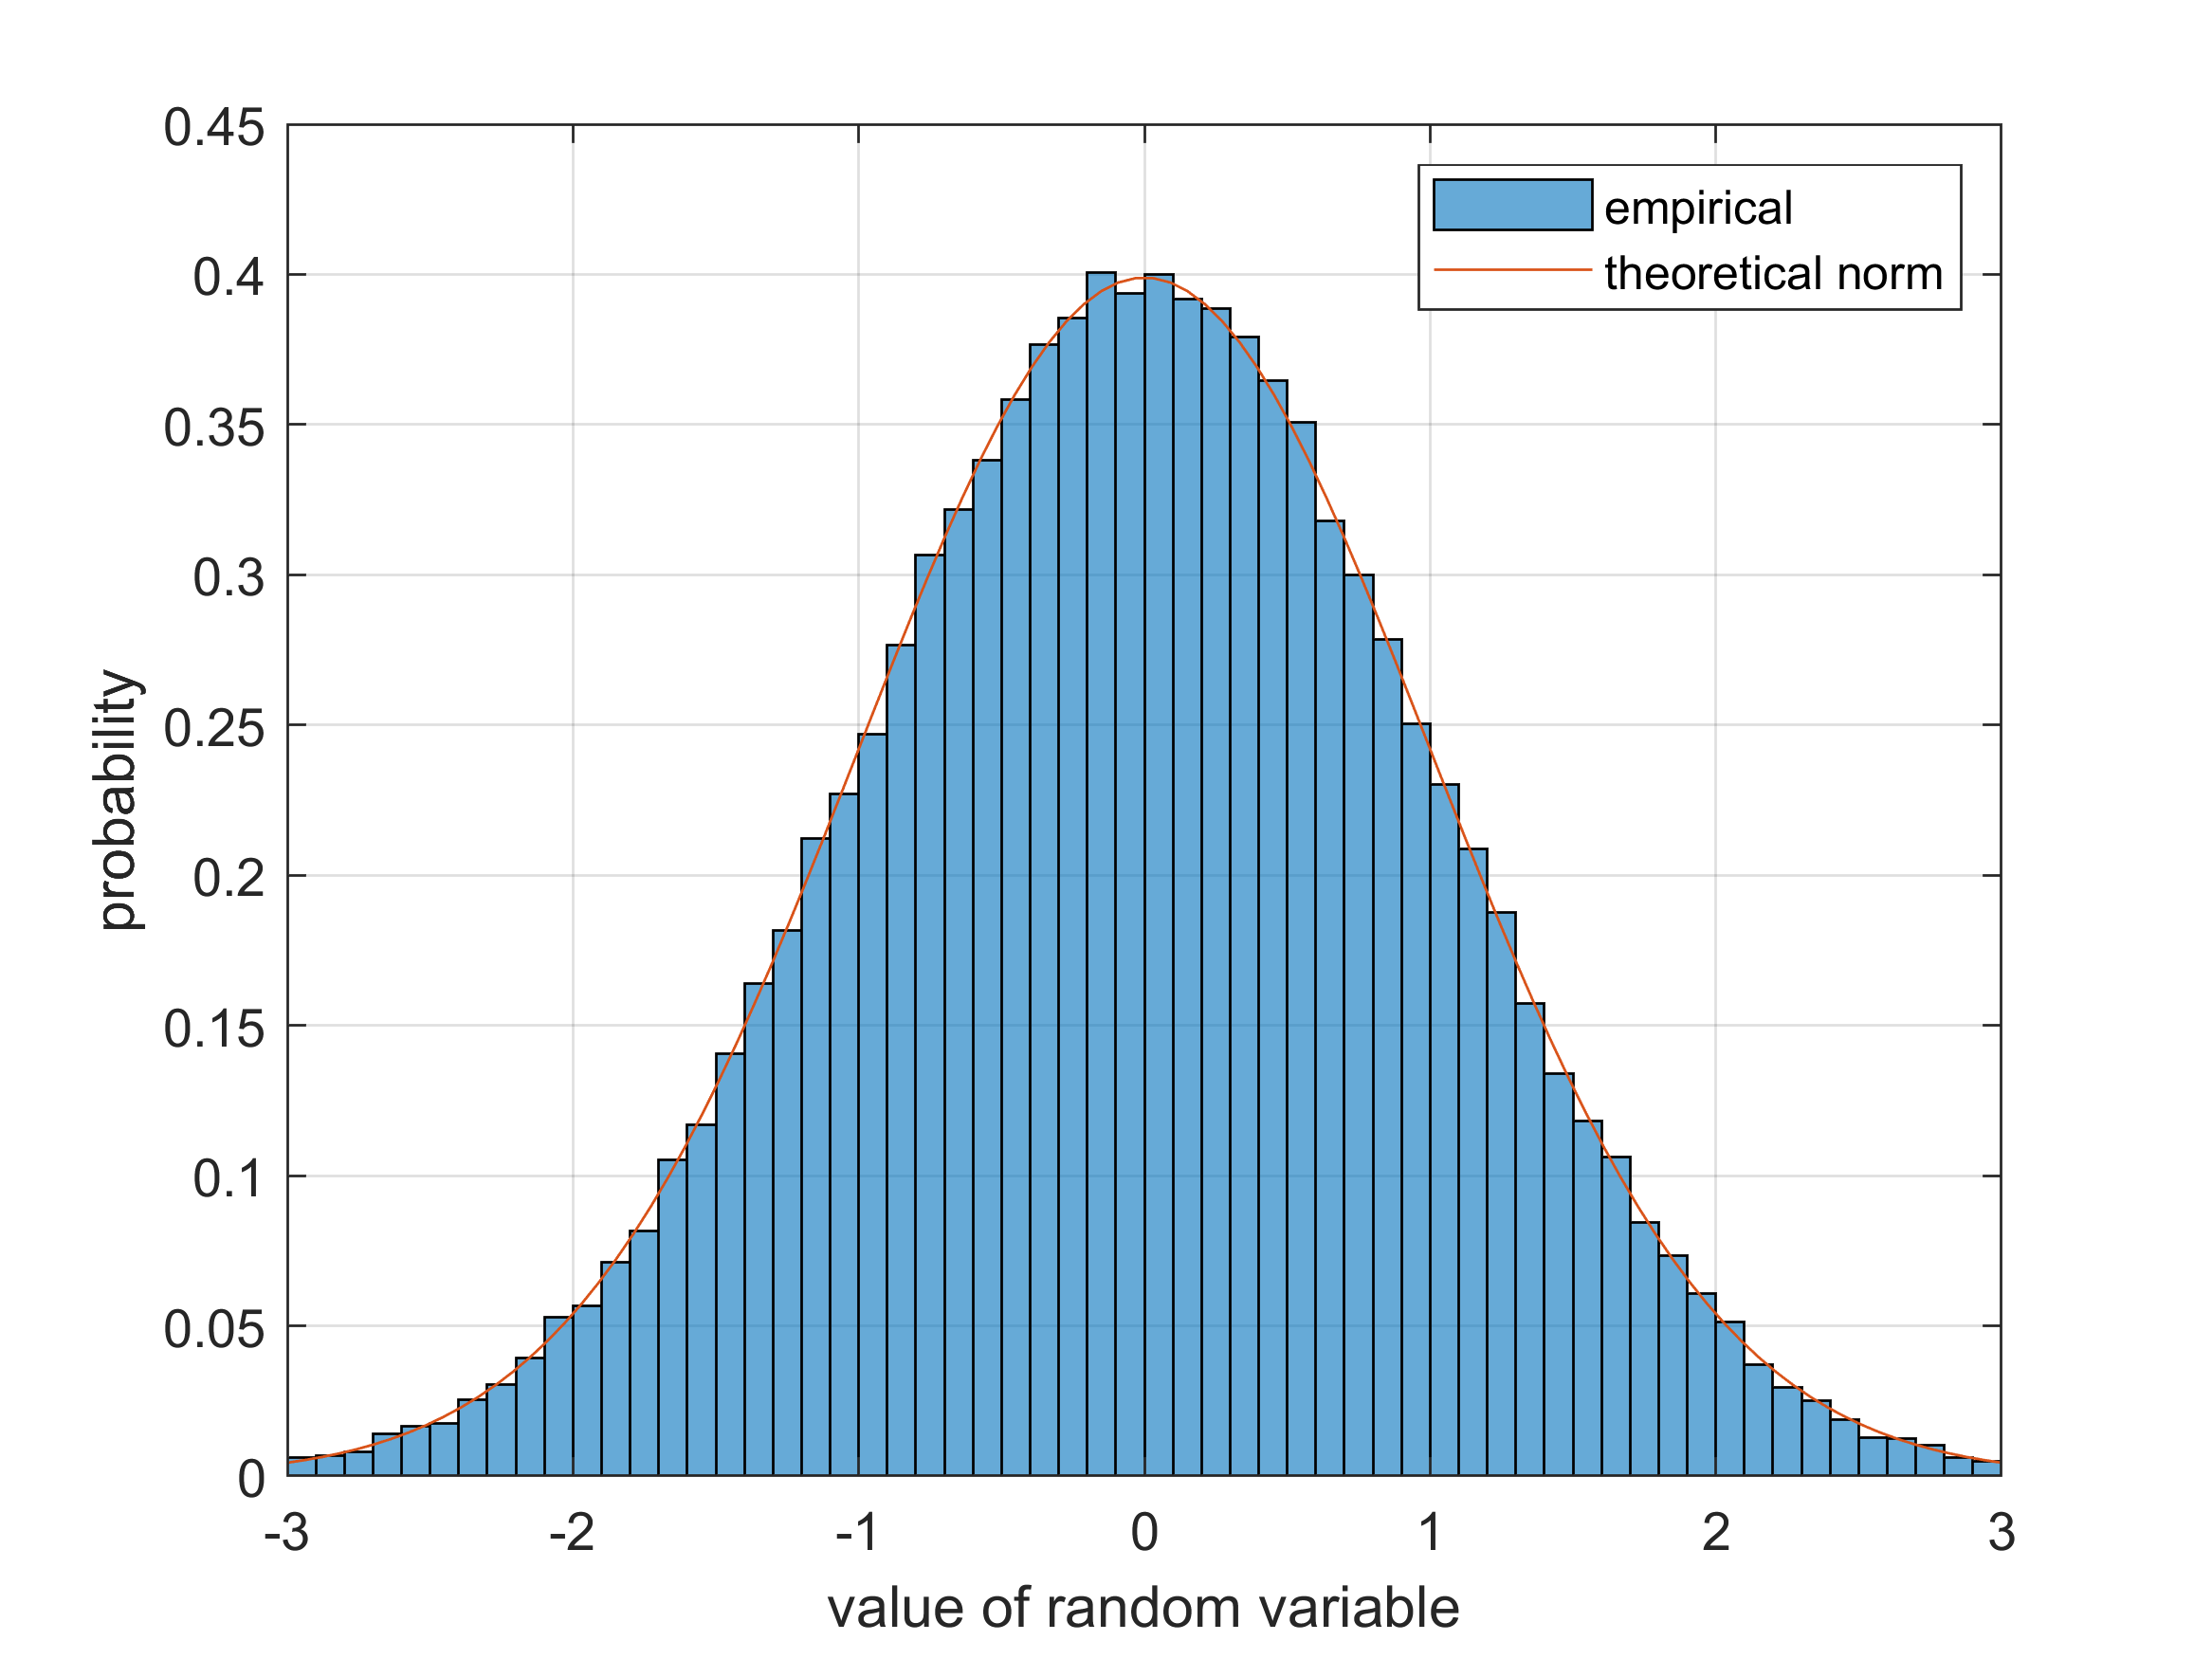
\includegraphics[width=0.6\textwidth]{../code/Task_3/pict/norm_vis_ksi_ex.png}
		\caption{Нормальное распределение, генерируемое с помощью перехода в полярные координаты.}
    \end{figure}
		
	\newpage
	Мы полагаем, что полученные выбороки распределены нормально. Проверим, что 
	математическое ожидание полученного нами распределения совпадает с нормальным, при помощи  
	одновыборочного двустороннего критерия Стьюдента. 
	Он применяется для проверки нулевой гипотезы о равенстве
	математического ожидания $\E(X)$ некоторому известному значению $m$.
	
	Для проверки построим статистику:
	$$
		t = \dfrac{\bar{X}-m}{s_X/\sqrt{n}},
	$$
	 где	$s^2_X$ --- несмещенная оценка дисперсии.

	\textbf{Принятие решения по критерию Стьюдента:}

	Если статистика $t$ по абсолютному значению
	не превышает квантиль $t(\alpha/2, n-1)$ распределения Стьюдента,
	то нулевая гипотеза $H_{0}$ о равенстве математических ожиданий принимается на уровне $\alpha$. 
	Иначе гипотеза отвергается. 
	
	\begin{table}[h!]
	\begin{center}
		\begin{tabular}{|c|c|c|c|}
			\hline $N$ & частота принятия гипотезы \\ \hline
				$10^2$ & 0.95  \\ \hline
				$10^3$ & 0.949 \\ \hline
				$10^4$ & 0.9506 \\ \hline
		\end{tabular}
		\caption{ \centering  Проверка равенства математических ожиданий нормального 
											и полученного распределений при размере выборки $10^5$ 
											и уровне значимости $\alpha=0.05.$}
	\end{center}
	\end{table}

	Проверим, что дисперсии полученных нами распределений совпадают друг с другом, при помощи  
	двустороннего критерия Фишера. 
	Он применяется для проверки нулевой гипотезы о равенстве
	дисперсий $\Var(X)$ и $\Var(Y)$ двух выборок из $n$ и $m$ элементов соответственно.
	\newpage
	Для проверки построим статистику:
	$$
		f = \frac{\hat{\sigma}_X^2}{\hat{\sigma}_Y^2},
	$$
	 где	$\hat{\sigma}_Z^2$ --- соответствующие выборочные дисперсии.

	\textbf{Принятие решения по критерию Фишера:}

	Если статистика $f$ не превышает квантиль $f(1-\alpha/2, n-1, m-1)$ распределения Фишера и
									 не меньше $f(\alpha/2, n-1, m-1)$, то нулевая гипотеза $H_{0}$ 
	о равенстве дисперсий $\Var(X)$ и $\Var(Y)$ принимается на уровне $\alpha$. 
	Иначе гипотеза отвергается. 
	
	\begin{table}[h!]
	\begin{center}
		\begin{tabular}{|c|c|c|c|}
			\hline $N$ & частота принятия гипотезы \\ \hline
				$10^2$ & 0.96  \\ \hline
				$10^3$ & 0.955 \\ \hline
				$10^4$ & 0.9499 \\ \hline
		\end{tabular}
		\caption{ \centering  Проверка равенства математических ожиданий нормального 
											и полученного распределений при размере выборки $10^5$ 
											и уровне значимости $\alpha=0.05.$}
	\end{center}
	\end{table}
	


\section{Задание 4}

\subsection{Постановка задачи}
    \begin{enumerate} 
        \item Построить датчик распределения Коши. 
        \item На основе датчика распределения Коши с помощью метода фон Неймана построить датчик
			стандартного нормального распределения. При помощи функции normal probability plot 
			убедиться в корректности построенного датчика 
			и обосновать наблюдаемую линейную зависимость. 
        \item Сравнить скорость моделирования стандартного нормального распределения в заданиях 3 и 4. 
    \end{enumerate}

\subsection{Решение задачи}
\subsubsection{Пункт 1}

	\begin{definition}
		Случайная величина $X$ имеет распределение Коши с параметрами $a$ и $b$, 
		если ее функция распределения имеет вид:
		$$
			F_X(x) = \dfrac{1}{\pi}\arctan \left( \dfrac{x-a}{b} \right) + \dfrac{1}{2}.
		$$	
	\end{definition}
	Поскольку фунция распределения $F_X(x)$ удовлетворяет условиям теоремы 2, воспользуемся этой 
	теоремой для моделирования случайной величины с распределением Коши. Обратная функция равна:
	$$
		F_X^{-1}(y) = a + b \tan \left( \pi \left( y - \dfrac{1}{2} \right) \right).
	$$
	Тогда по теореме 2 случайная величина $X=F_X^{-1}(Y)$, где $Y\sim U[0;1],$ имеет распределение Коши.

	\begin{figure}[h!]
		\centering
		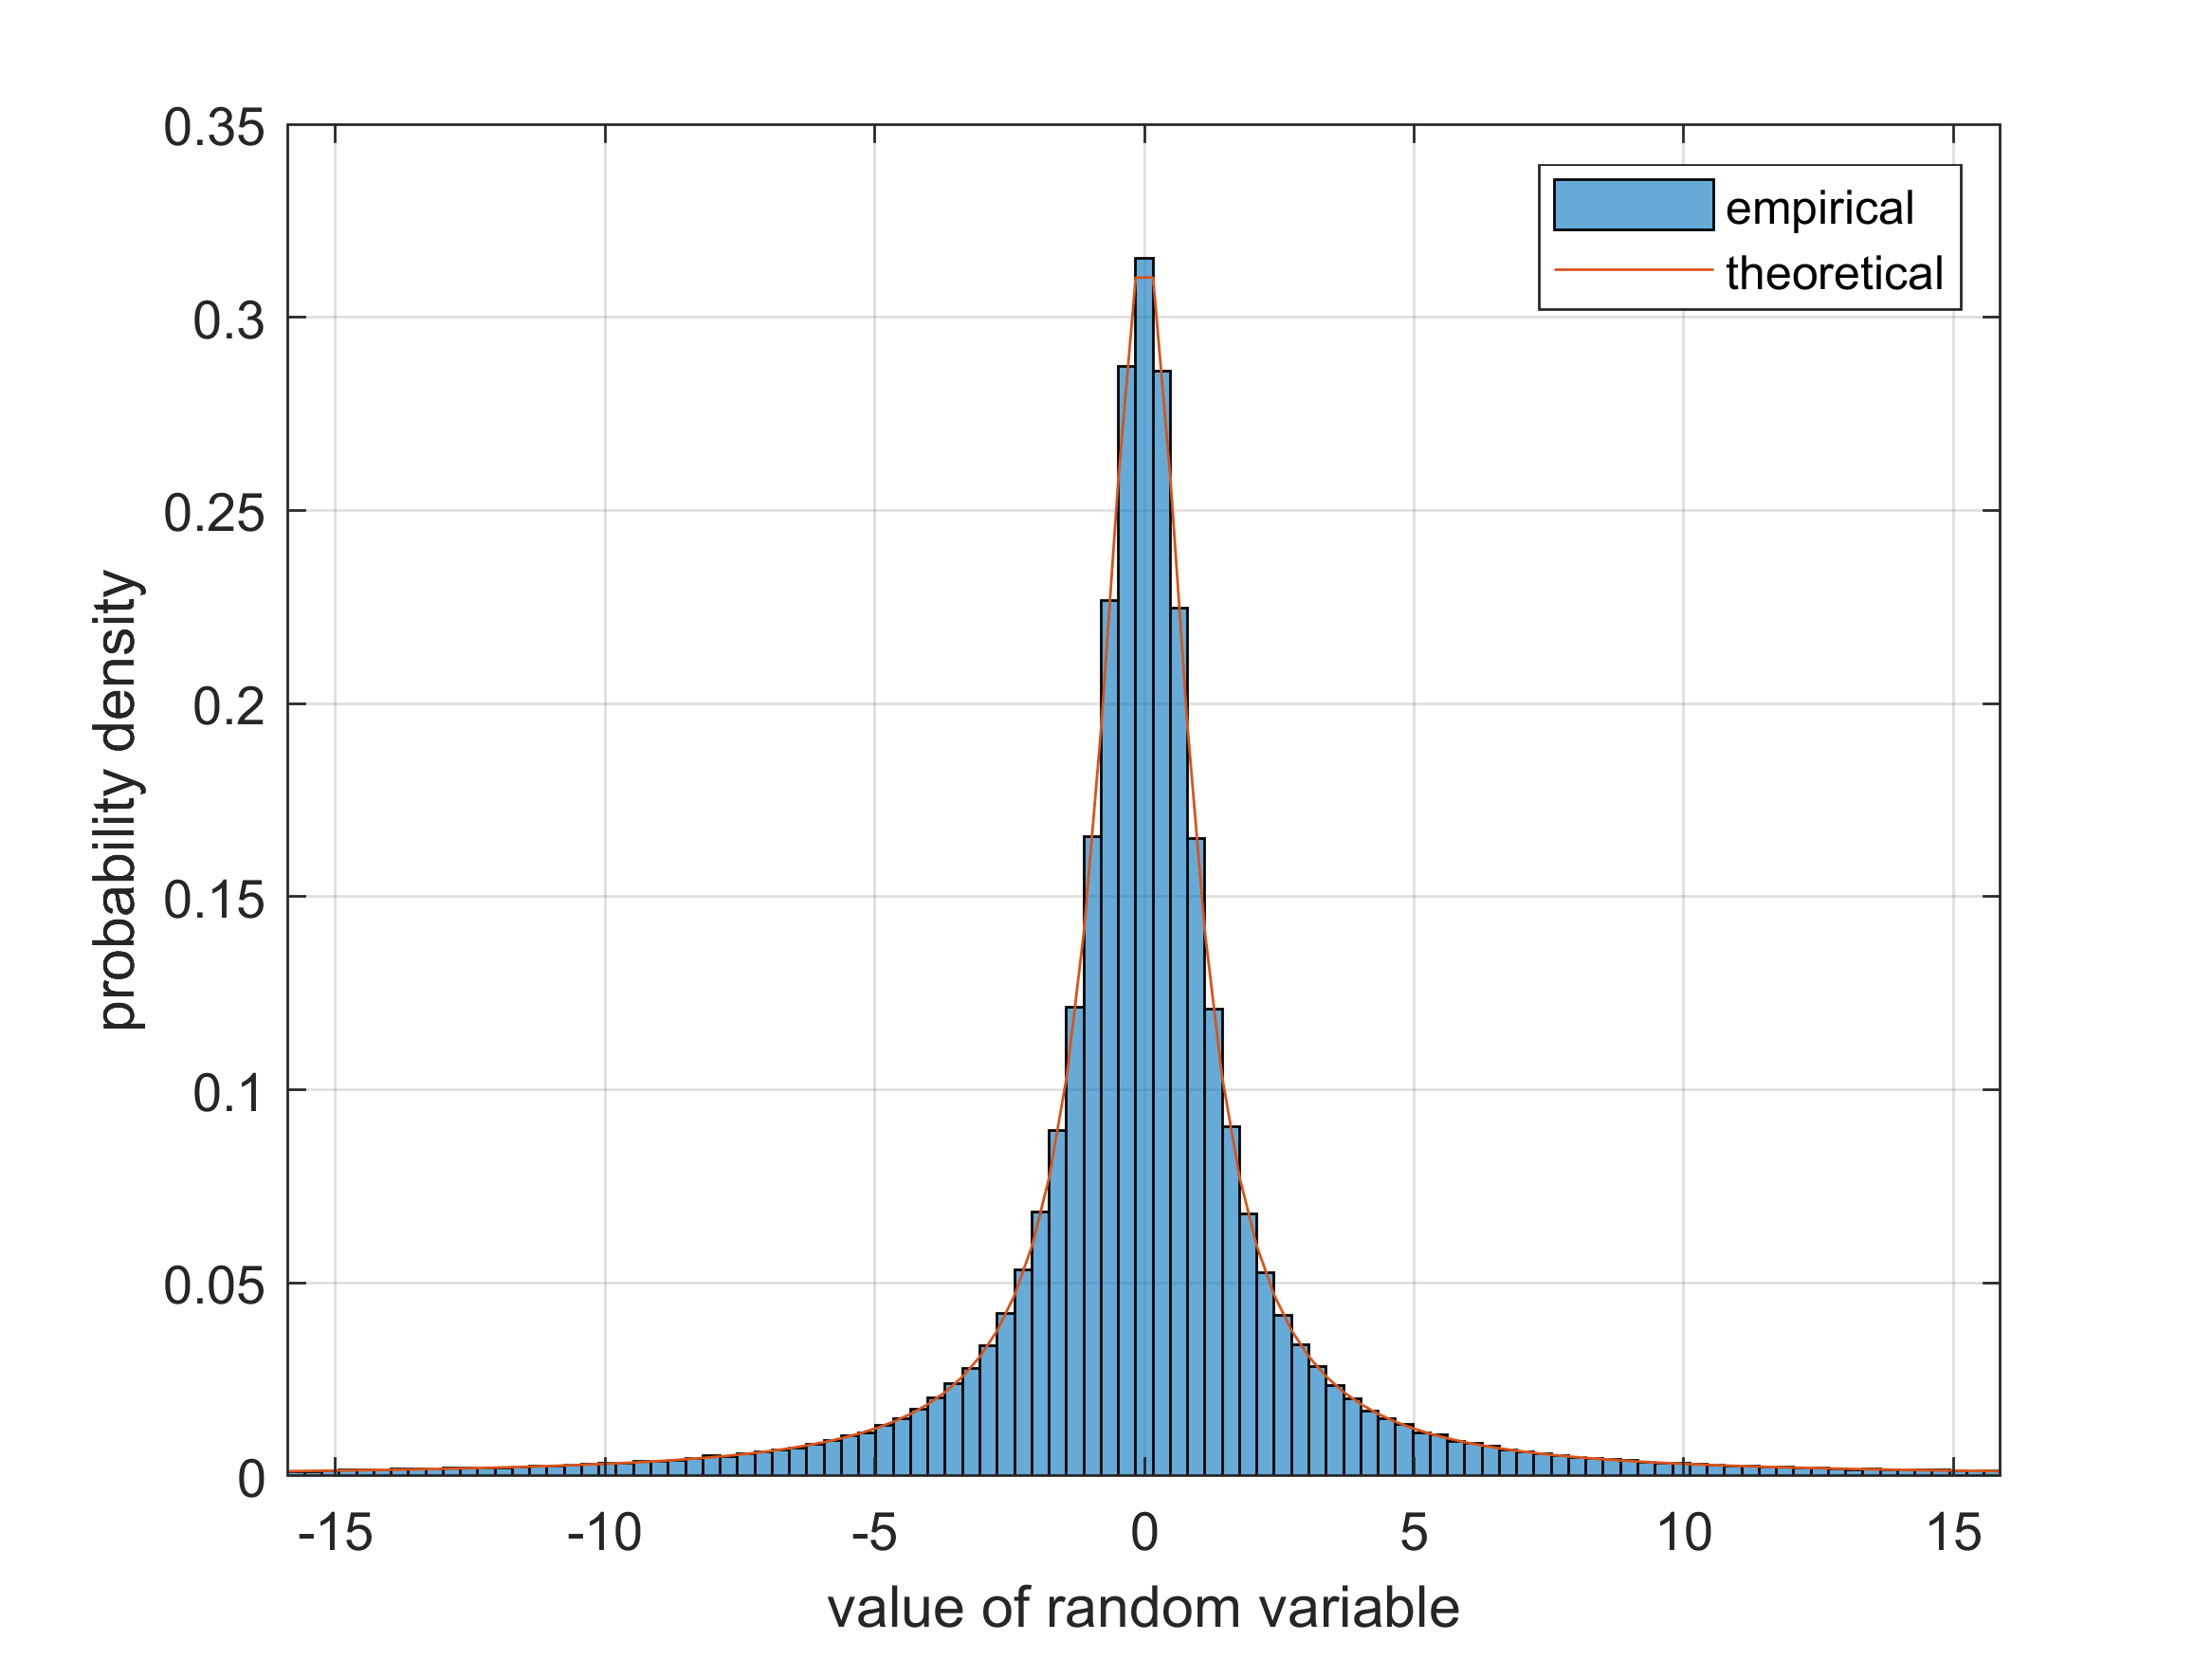
\includegraphics[width=0.6\textwidth]{../code/Task_4/pict/cauchy_vis_ex.png}
		\caption{Распределение Коши с параметрами $a=0, b =1, n=10^6.$}
    \end{figure}

\subsubsection{Пункт 2}
	
	Пусть имеется некоторое вещественное вероятностное пространство $(E, \mathcal{E})$, на котором заданы 
	абсолютно непрерывные распределения $\P$ и $\Q$. Пусть выполнено условие: 
	$$
		 \exists\, k >1: \Q(A) \leqslant k \P(A)\quad \forall A\in \mathcal{E},
	$$
	из которого следует, что $\Q<<\P$, т.е. $\Q$ абсолютно непрерывно относительно $\P$. По теореме 
	Радона-Никодима, отсюда также следует, что существует производная 
	Радона-Никодима $\gamma(x):$
	$$
		\gamma(x) = \dfrac{d\Q}{d\P} \leqslant k,
	$$
	где $d\Q$ и $d\P$ --- плотности  соответствующих распределений.

	Предположим, что у нас есть датчик случайной величины $X$  с распределением $\P$ и выполнено
	условие выше.	Будем моделировать $\Q$, следуя алгоритму метода исключения фон-Неймана:
	\begin{enumerate}
		\item Подбираем $k>1: d\Q(x)\leqslant kd\P(x), \quad \forall x \in \mathbb{R},$
		\item Получим значение $x$ случаной величины $X$,
		\item Получим значение $y$ случаной величины
				 $Y(x) \sim Bern\left( \dfrac{d\Q(x)}{kd\P(x)} \right)$,
		\item Если $y=1$, то $x$ из моделируемого распределения с плотностью 
				$d\Q(x)$,\newline иначе --- возвращаемся к пункту 2.
	\end{enumerate}
	\newpage
	Обоснуем изложенный алгоритм. Пусть $\nu\sim Bern\left(\frac{1}{k}\right)$, тогда:
	\begin{enumerate}
			\item $p(\nu =1|X =x ):= \dfrac{\gamma(x)}{k} \text{, т.е. данная плотность соответствует }
											 Bern\left( \dfrac{d\Q(x)}{kd\P_X(x)} \right) $,
			\item 	$$ 
							\P(X \in B| \nu = 1) =\dfrac{\P(\{X\in B\} \cap \{\nu=1 \})}{\P(\nu=1 )} =
						$$
						$$
							= \left\{ \begin{gathered}
							 	 \P(\{X\in B\} \cap \{\nu=1 \})= 
								\int\limits_B p(\nu=1|X=x) \P_X(dx) =\\
								= \int\limits_B \dfrac{\gamma(x)}{k}  \P_X(dx)
								= \dfrac{1}{k}\int\limits_B \gamma(x) \P_X(dx) =
								\dfrac{1}{k} \Q(B) 					
							\end{gathered}	\right\}	= \dfrac{\Q(B)}{k\,\P(\nu=1)} = \Q(B),
						$$			
	\end{enumerate}
	что доказывает используемый метод.

	Запишем плотность стандартного нормального распределения $q(x)$ и плотность
	распределения Коши $p(x)$:
	$$
		\begin{gathered}
			q(x) = \dfrac{1}{\sqrt{2\pi}}e^{-\frac{x^2}{2}}, \\
			p(x) = \dfrac{1}{\pi}\dfrac{b}{(x-a)^2+b^2}.
		\end{gathered}
	$$
	Для данных распределений выполняются все условия метода исключения фон-Неймана, 
	поэтому будем генерировать 
	стандартное нормальное распредедение с помощью распределения Коши $K(0,1)$, 
	а $k$ положим равным $k =\sqrt{\dfrac{2\pi}{e}} >1.$
	
	\begin{figure}[h!]
		\centering
		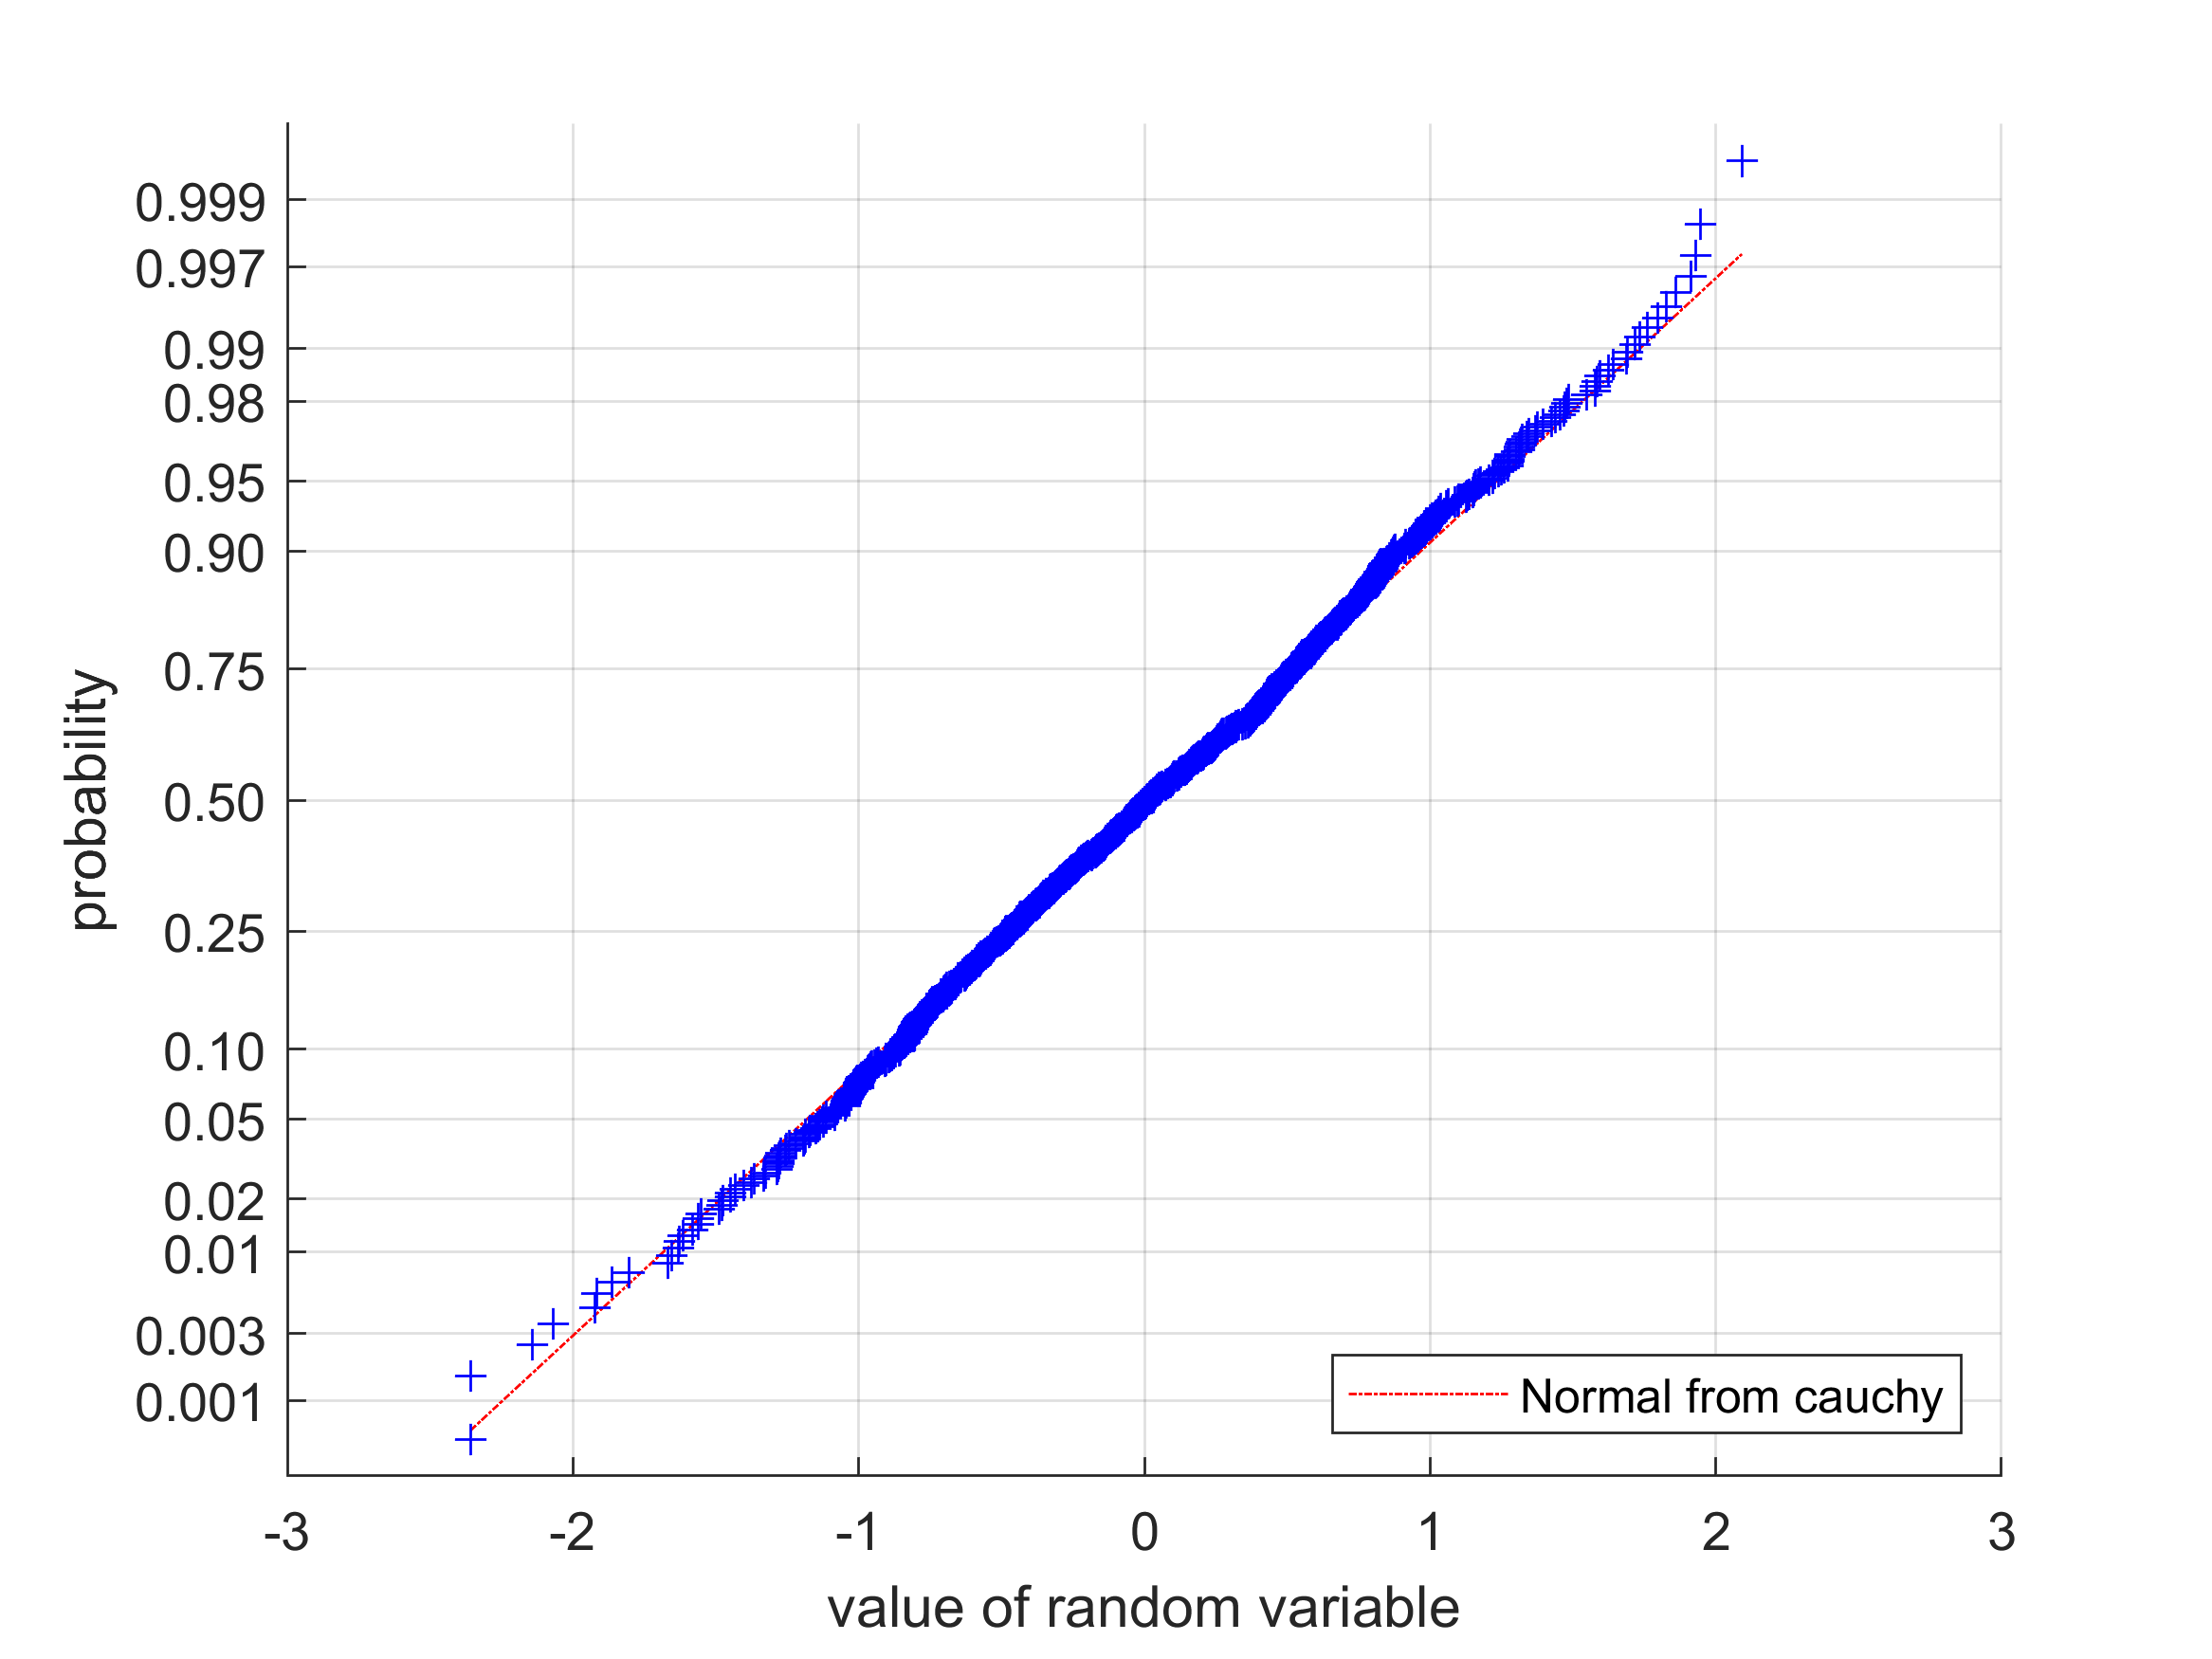
\includegraphics[width=0.6\textwidth]{../code/Task_4/pict/norm_ex.png}
		\caption{Стандартное нормальное распределение, генерируемое методом фон-Неймана, $n=10^4.$}
    \end{figure}	

	Исследуем, как будут распределены с.в. $Y=\mu+\sigma X$, где $X\sim N(0,1)$:
	$$
		\varphi_{\mu+\sigma X}(t) = \E e^{it(\mu+\sigma x)} = \E e^{it\sigma x}e^{it\mu} =
		e^{it\mu} \varphi_X(\sigma t) = e^{it\mu} e^{\frac{t\sigma^2}{2}} =\varphi_Z(t), 
	$$
	где $Z\sim N(\mu, \sigma^2).$ Соответсвенно, с.в. $Y$ будет распределена нормально 
	$Y\sim  N(\mu, \sigma^2)$. 

	\newpage 
		На графике коэффициент $\mu$ будет отвечать за сдвиг вдоль оси $x$, а 
	коэффициент $\sigma$ --- за коэффициент наклона прямой (чем больше $\sigma$, тем более пологий
	график):
	\begin{figure}[h!]
		\centering
		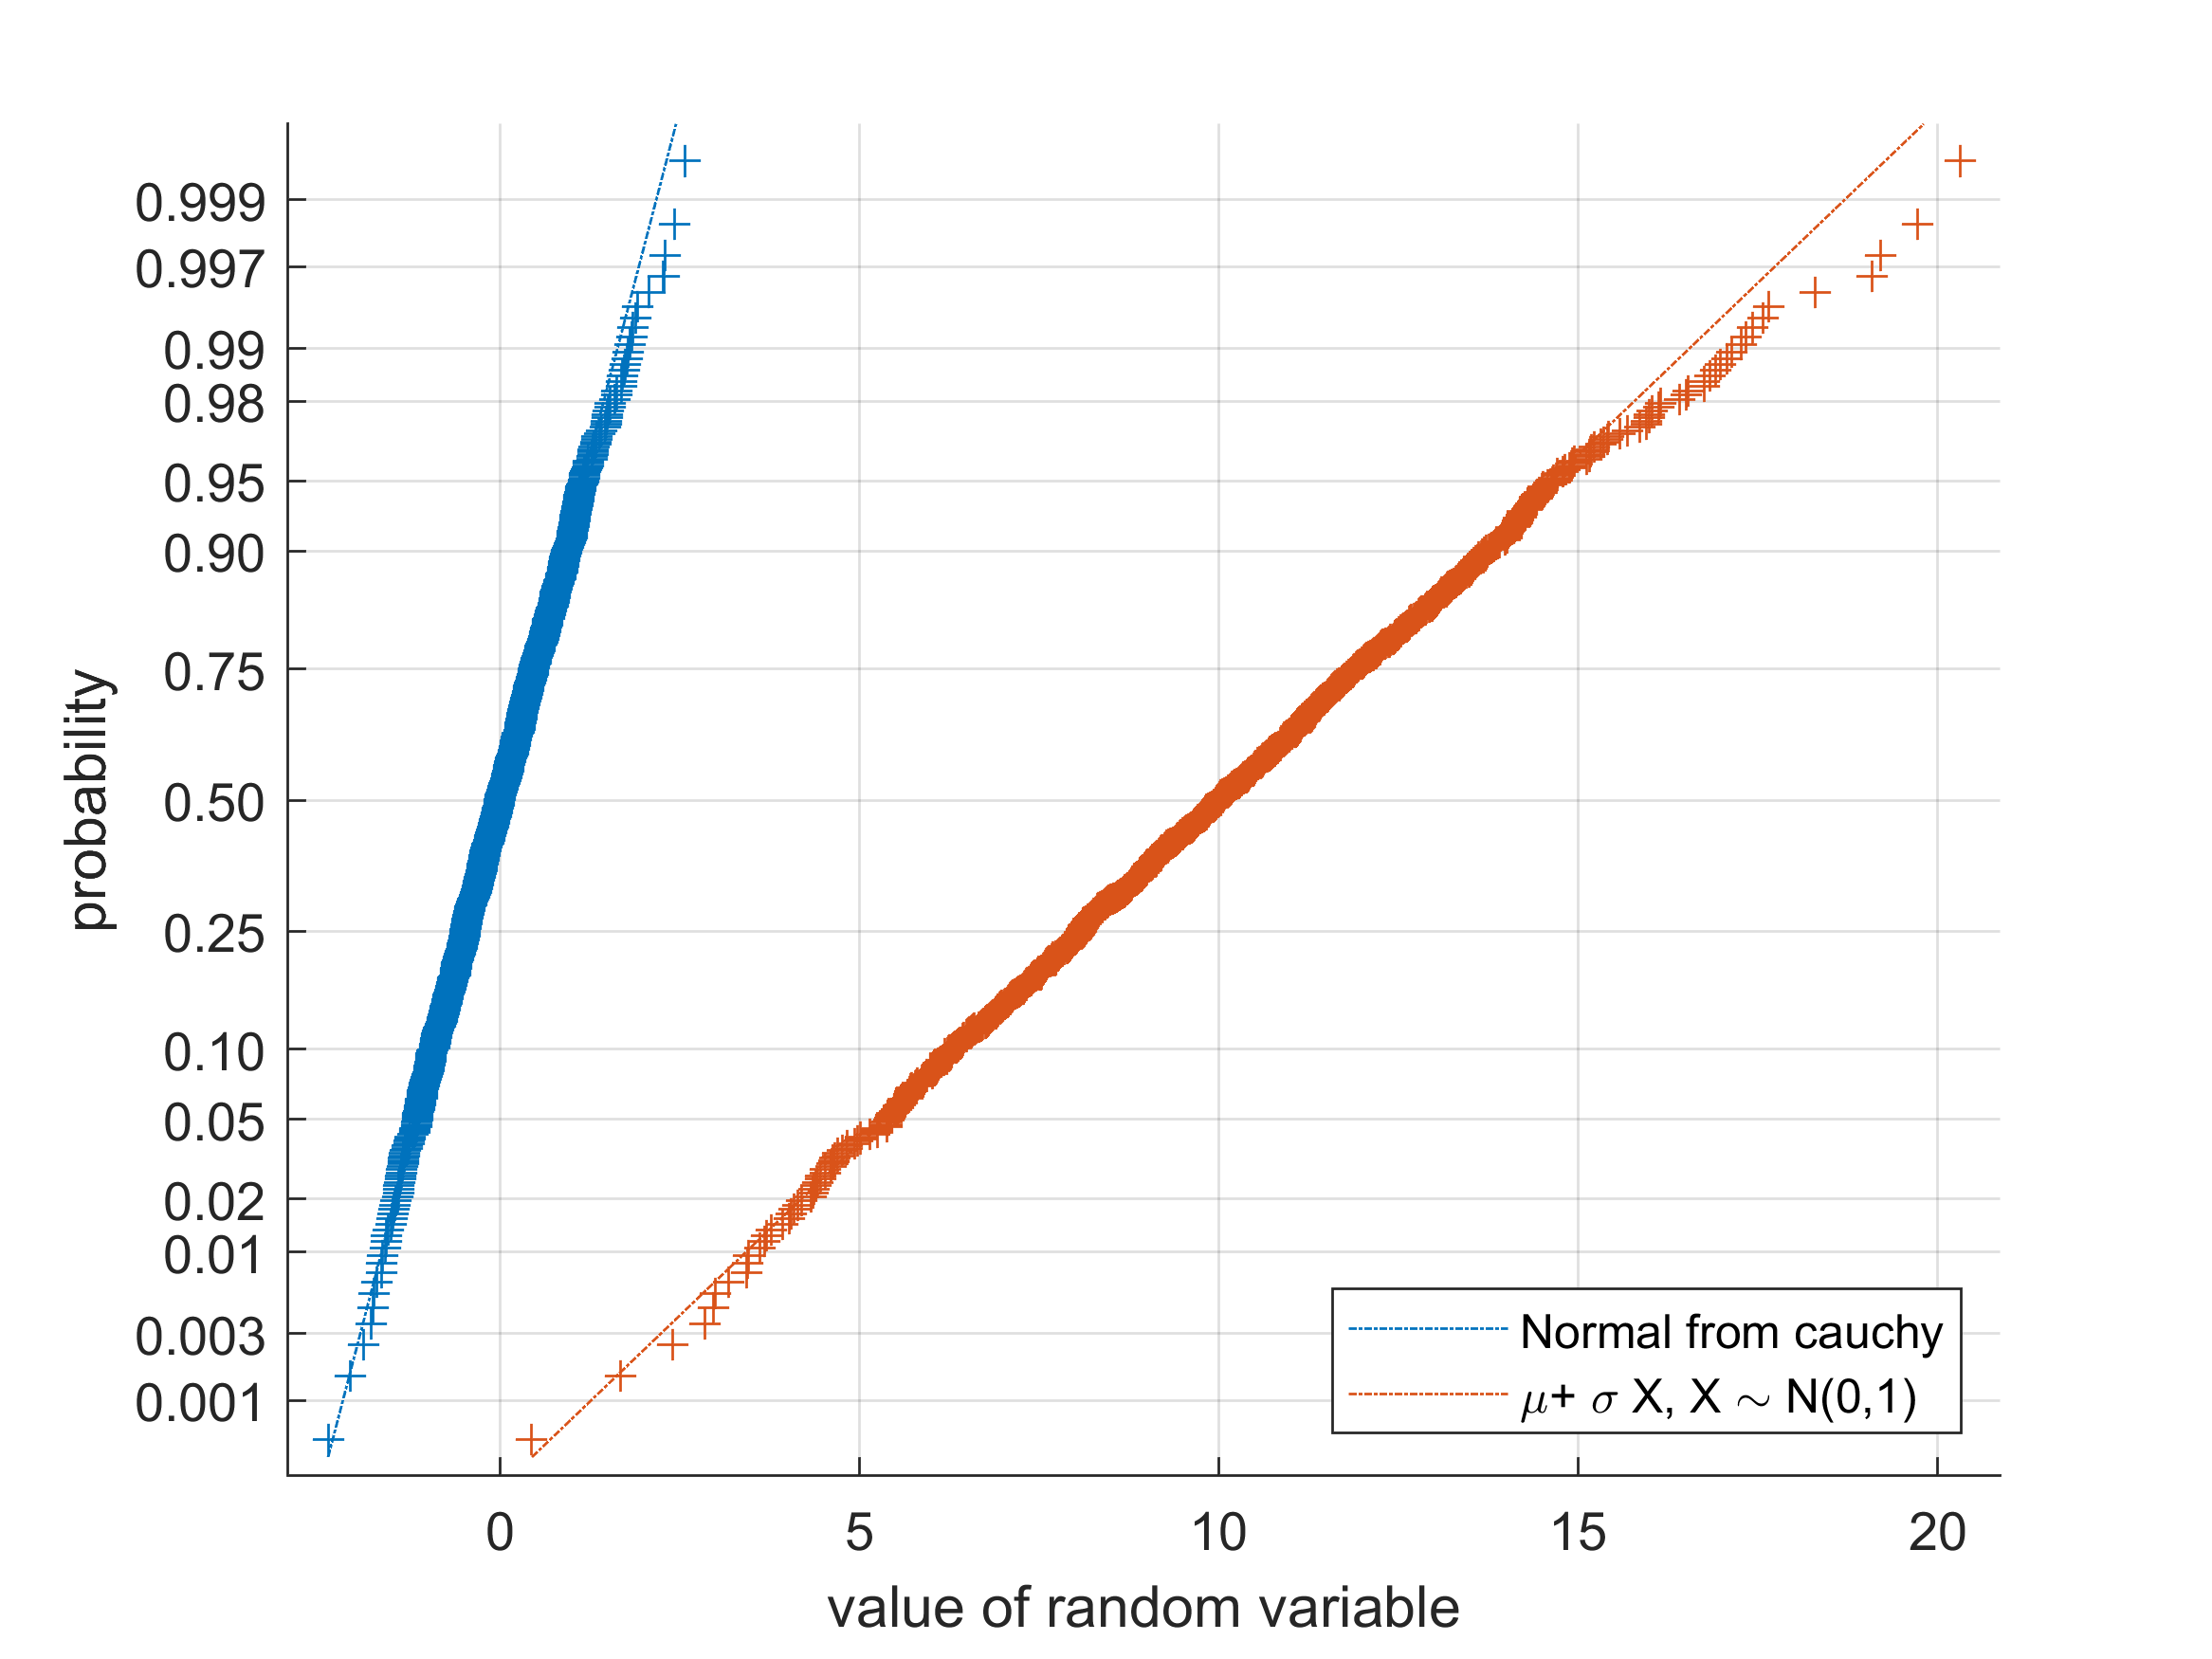
\includegraphics[width=0.6\textwidth]{../code/Task_4/pict/norm_2_ex.png}
		\caption{ \centering Результат сдвига и сжатия с.в. $X\sim N(0,1)$, полученной методом фон-Неймана. 
						 \newline Параметры: $\mu =10, \sigma =4,  n=10^4.$ }
    \end{figure}
	
	Функция, normplot, по-сути, строит линейную часть функции распределения нормального распределения, а 
	форма функций распределения других распределений отличается от нормального. Например, для
	экспоненциального распределения, прямая на графике не получится:

	\begin{figure}[h!]
		\centering
		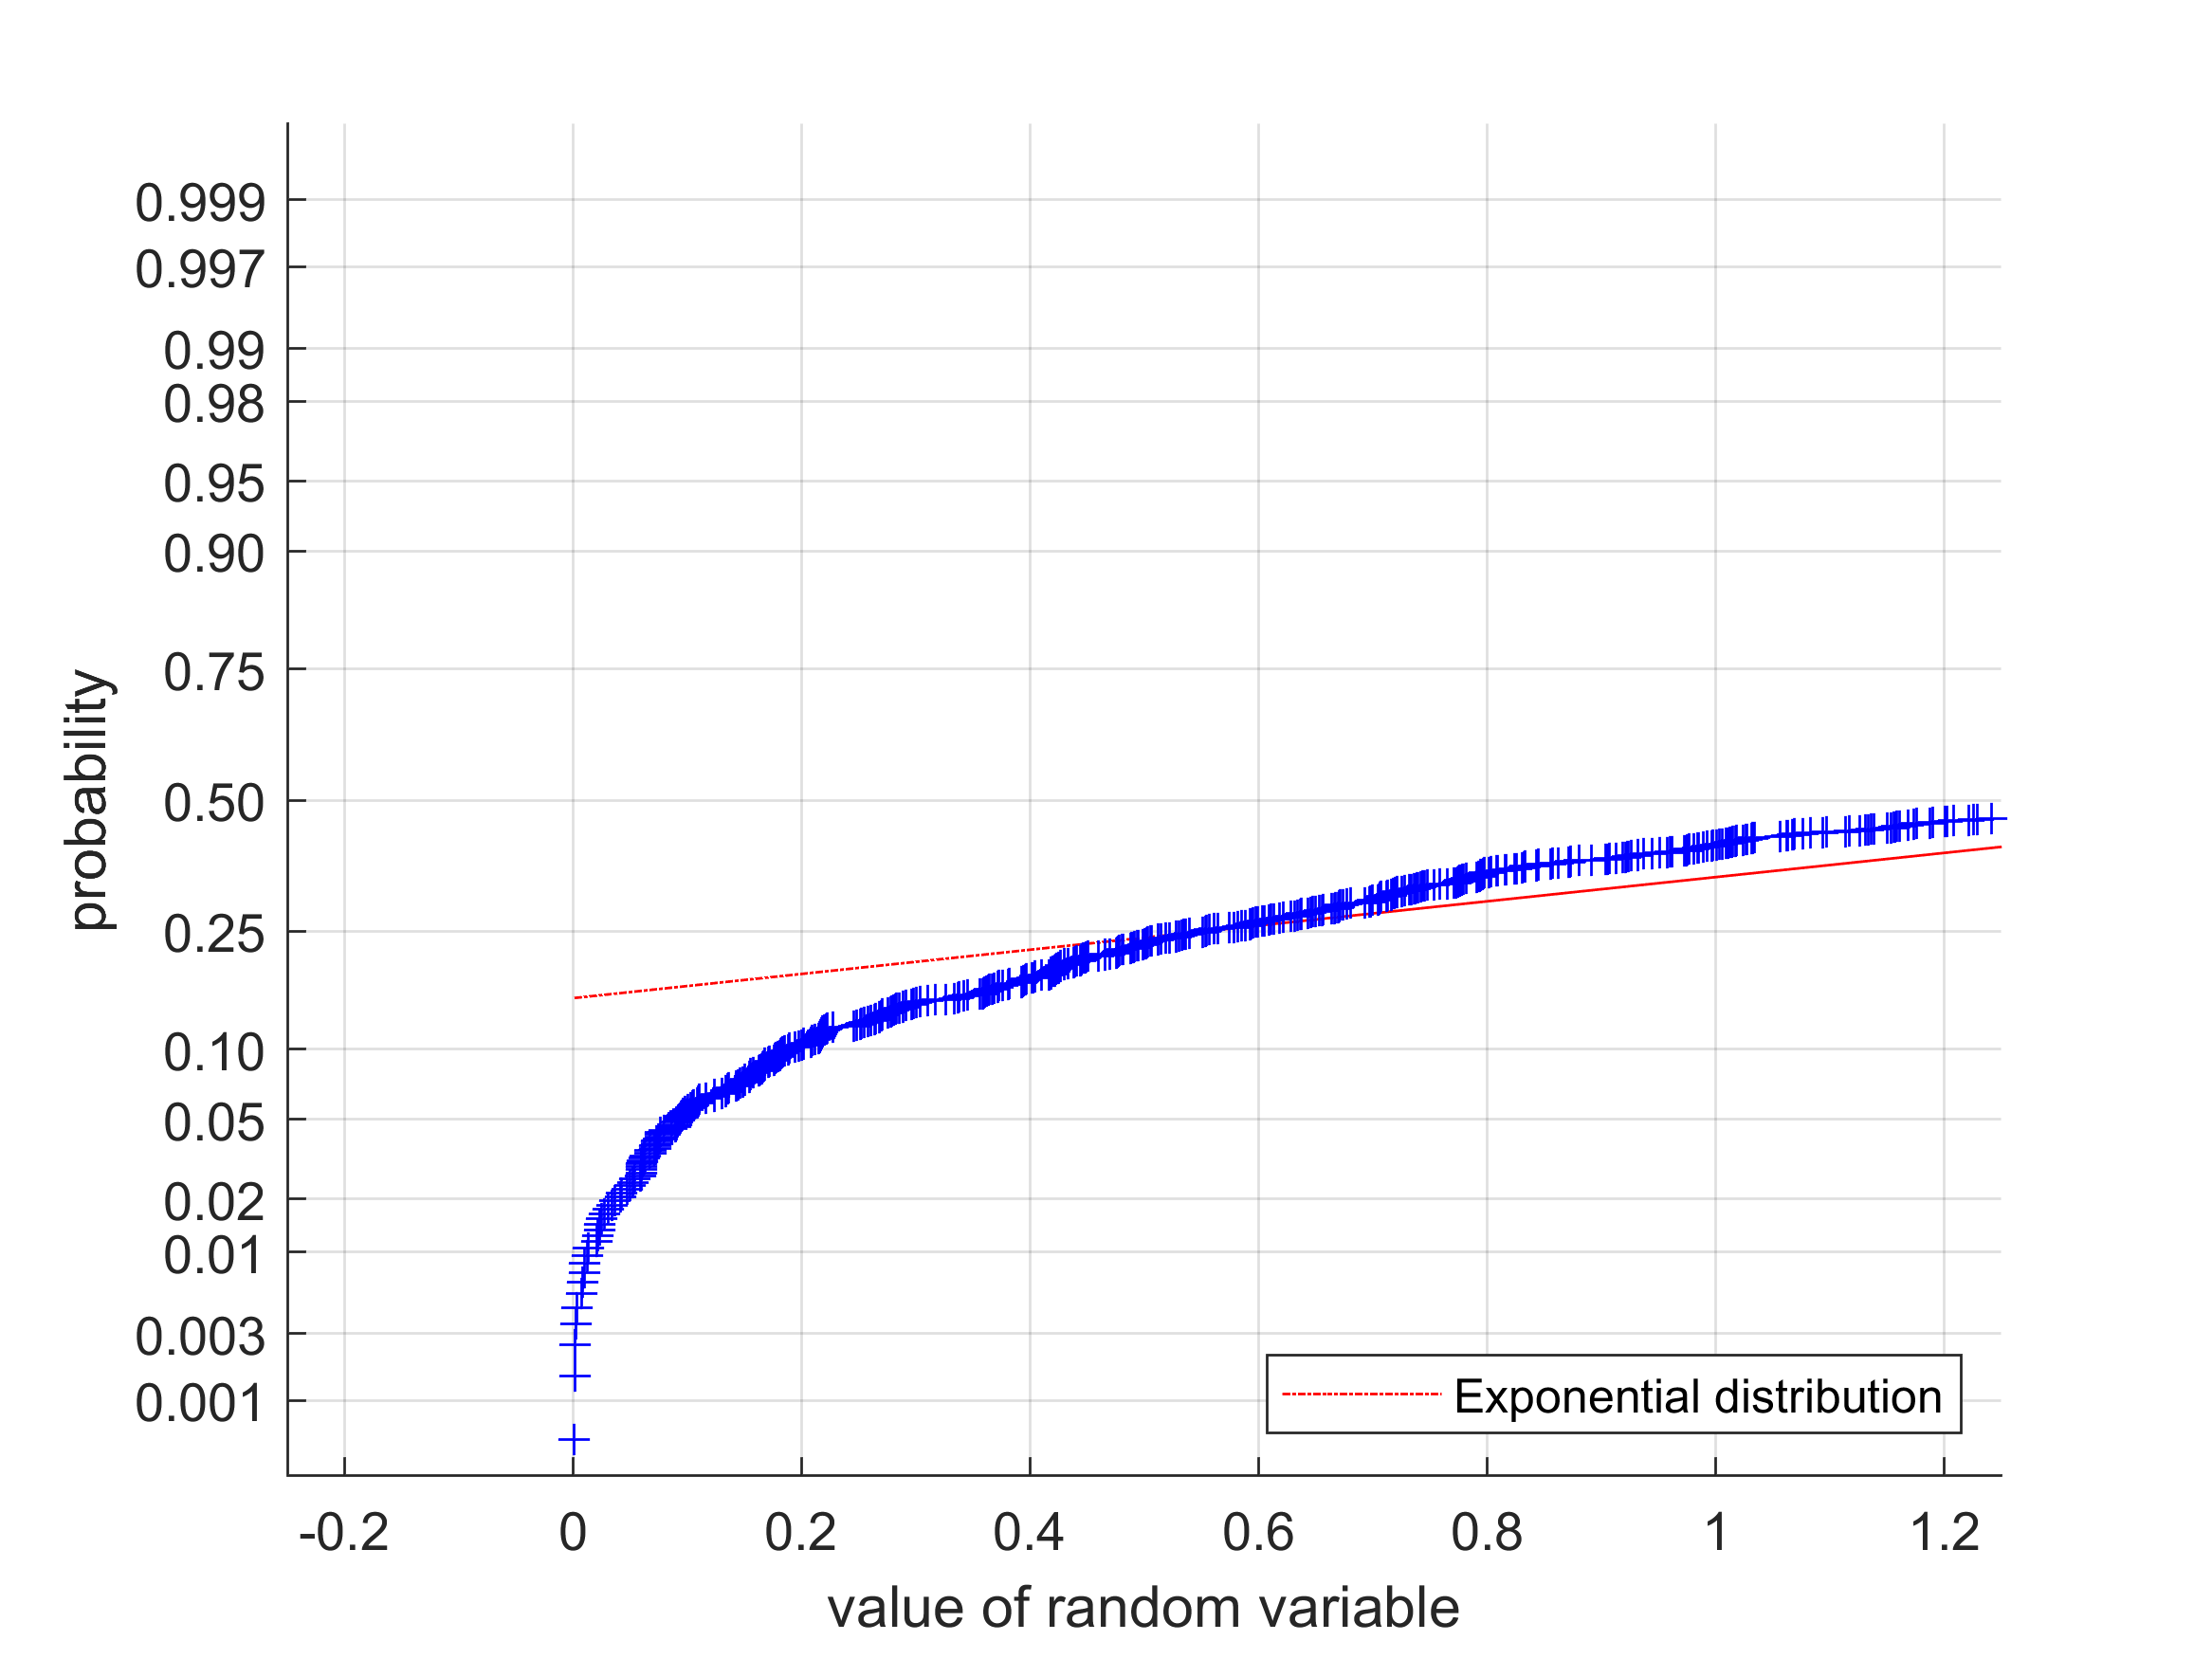
\includegraphics[width=0.6\textwidth]{../code/Task_4/pict/norm_exp_ex.png}
		\caption{Результат применения $normplot$ к экспоненциальному распределению, $n=10^3.$}
    \end{figure}
	
\newpage
\subsubsection{Пункт 3}
	\noindent
	Сравним скорости моделирования стандартного нормального распределения в заданиях 3 и 4:
	\begin{table}[h!]
	\begin{center}
		\begin{tabular}{|c|c|c|c|}
			\hline $N$ & Newmann & Polar   \\ \hline
				$10$ 	&  0.0016919  &  0.00076547\\ \hline
				$10^3$ & 0.00024191  &  0.00005675 \\ \hline
				$10^5$ & 0.013248  &   0.0036173 \\ \hline
				$10^7$ & 1.3195 &  0.42665 \\ \hline
		\end{tabular}
		\caption{ \centering  Среднее время генерации $N$ случайных величин при $10^3$ тестах.}
	\end{center}
	\end{table}

	Как можем видеть, моделирование стандартно нормально рапределенных случайных величин
	методом фон-Неймана  меделенее, чем моделирование парами.
	
\newpage
\section{Задание 5}

\subsection{Постановка задачи}
    \begin{enumerate} 
        \item Пусть $X_i \sim N(\mu, \sigma^2)$. Убедиться эмпирически в справедливости ЗБЧ и ЦПТ,
			 т.е. исследовать поведение суммы $S_n$ и эмпирического распределения величины 
			$$\sqrt{n}\Big( \dfrac{S_n}{n} - a\Big).$$
        \item Считая $\mu$ и $\sigma$ неизвестными для пункта 1 построить доверительные интервалы
			для среднего и дисперсии. 
        \item Пусть $X_i \sim K(a, b)$ имеет распределение Коши со сдвигом a и масштабом b. 
			Проверить эмпирически, как ведут себя суммы $S_n/n$. Результат объяснить,
			а также найти закон распределения данных сумм.
    \end{enumerate}
\subsection{Решение задачи}
\subsubsection{Пункт 1}

	\begin{theorem}{\textbf{ЗБЧ}}
    	\newline
        Пусть $X_1, X_2, \ldots, X_n$ --- независимые случайные величины и дисперсия  каждой из них существует
		и ограничена сверху некоторой константой: $\forall i: 1\leqslant i \leqslant n$ $\exists \, \Var X_i \leqslant C$. 
		Тогда
        $$
            \forall \varepsilon>0  \quad 
			\P\left(\left| \dfrac{X_1 + \ldots + X_n }{n} - \dfrac{\E X_1 + \ldots + \E X_n }{n}  \right| <
																																		 \varepsilon \right) 
            \xrightarrow[]{n \rightarrow \infty} 1
        $$
    \end{theorem}

	\begin{figure}[h!]
		\centering
		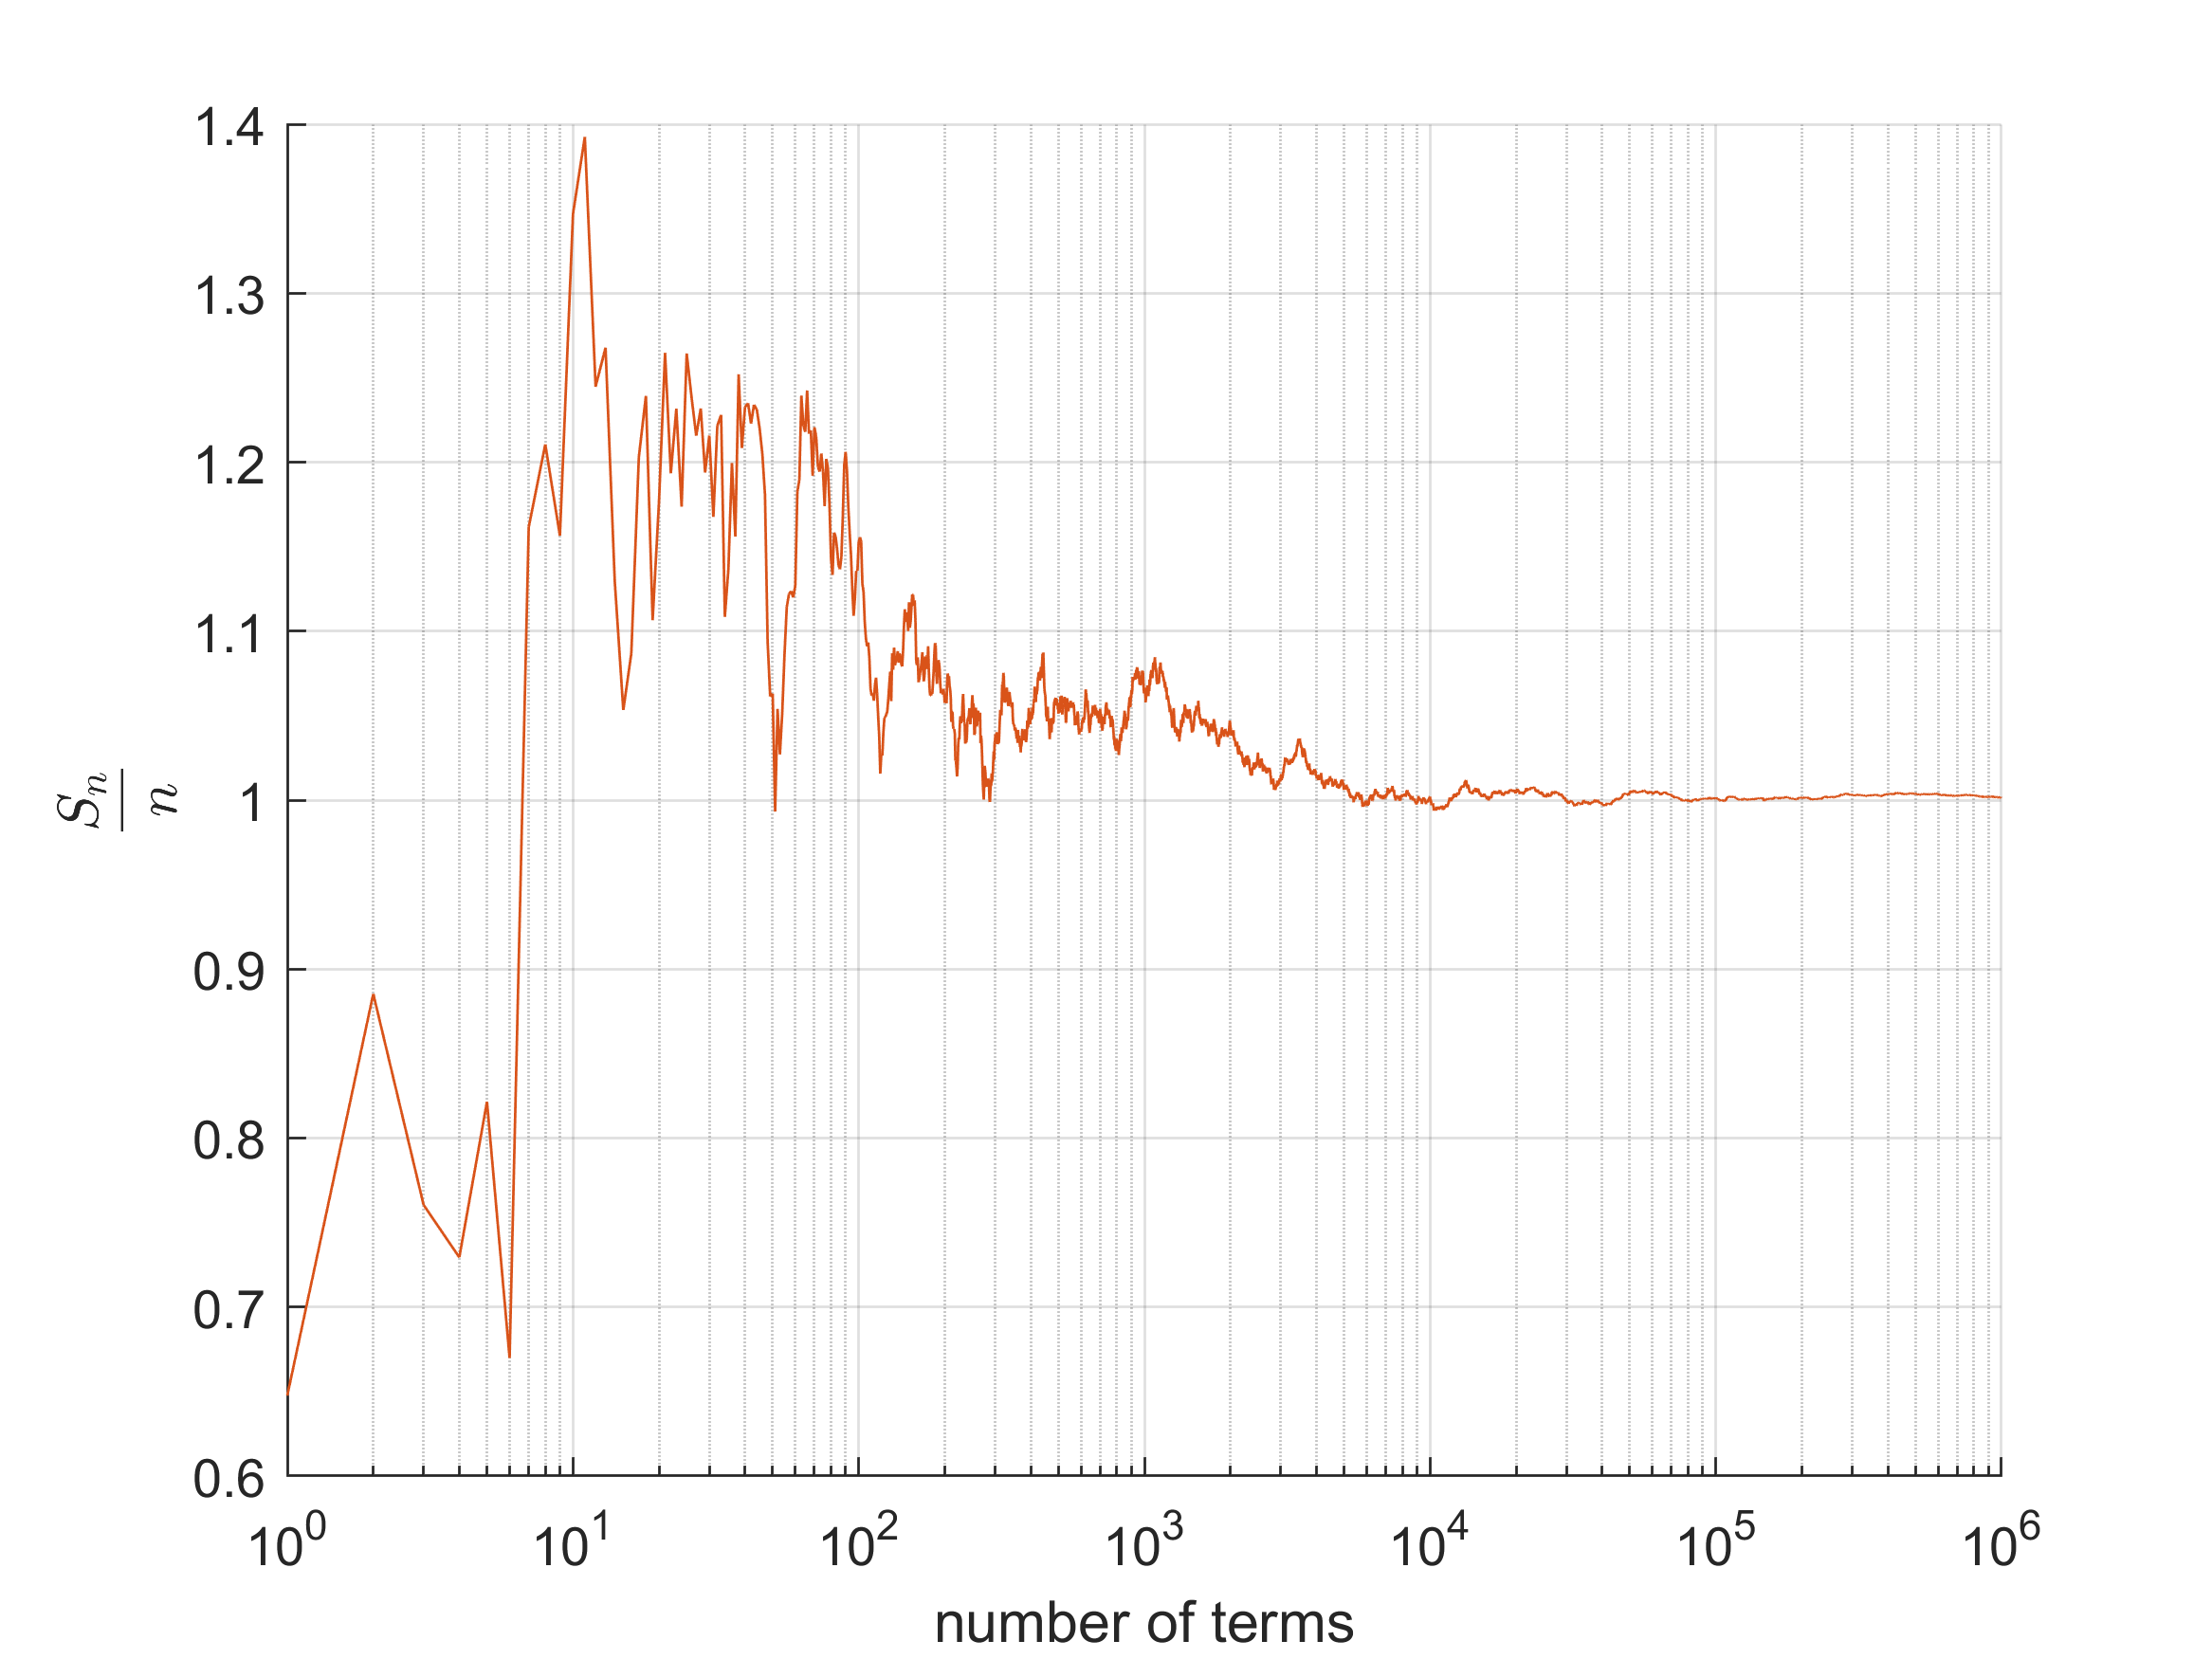
\includegraphics[width=0.6\textwidth]{../code/Task_5/pict/LLN_ex.png}
		\caption{Демонстрация ЗБЧ для выборки размером $n=10^6$ при $\mu = 1$.}
    \end{figure}

	\newpage
 	\begin{theorem}{\textbf{ЦПТ}}
	    \newline
        Пусть $X_1, X_2, \ldots, X_n$ --- последовательность невырожденных н.о.р.с.в.  
		с $\E X_1^2<\infty$, $S_n = X_1 + \ldots + X_n$. Тогда для $\forall x \in \mathbb{R}$ имеем
        $$
            \P\left(\frac{S_n-\E S_n}{\sqrt{\Var S_n}}\leqslant x\right) 
            \xrightarrow[]{n \rightarrow \infty} \Phi(x) = \frac{1}{\sqrt{2\pi}}
                                \int\limits^{x}_{-\infty}e^{-\frac{z^2}{2}}dz.
        $$
	 \end{theorem}
	В нашем формулировке при $ \E X_1 = a, \Var X_1 = \sigma^2 $ это преобразуется в 
	$$
		\P\left(\sqrt{n}\left(\frac{S_n}{n} -a\right) \leqslant x\right) 
            \xrightarrow[]{n \rightarrow \infty} \frac{1}{\sqrt{2\pi}\sigma}
                                \int\limits^{x}_{-\infty}e^{-\frac{z^2}{2\sigma^2}}dz.
	$$
   
	\begin{figure}[h!]
		\centering
		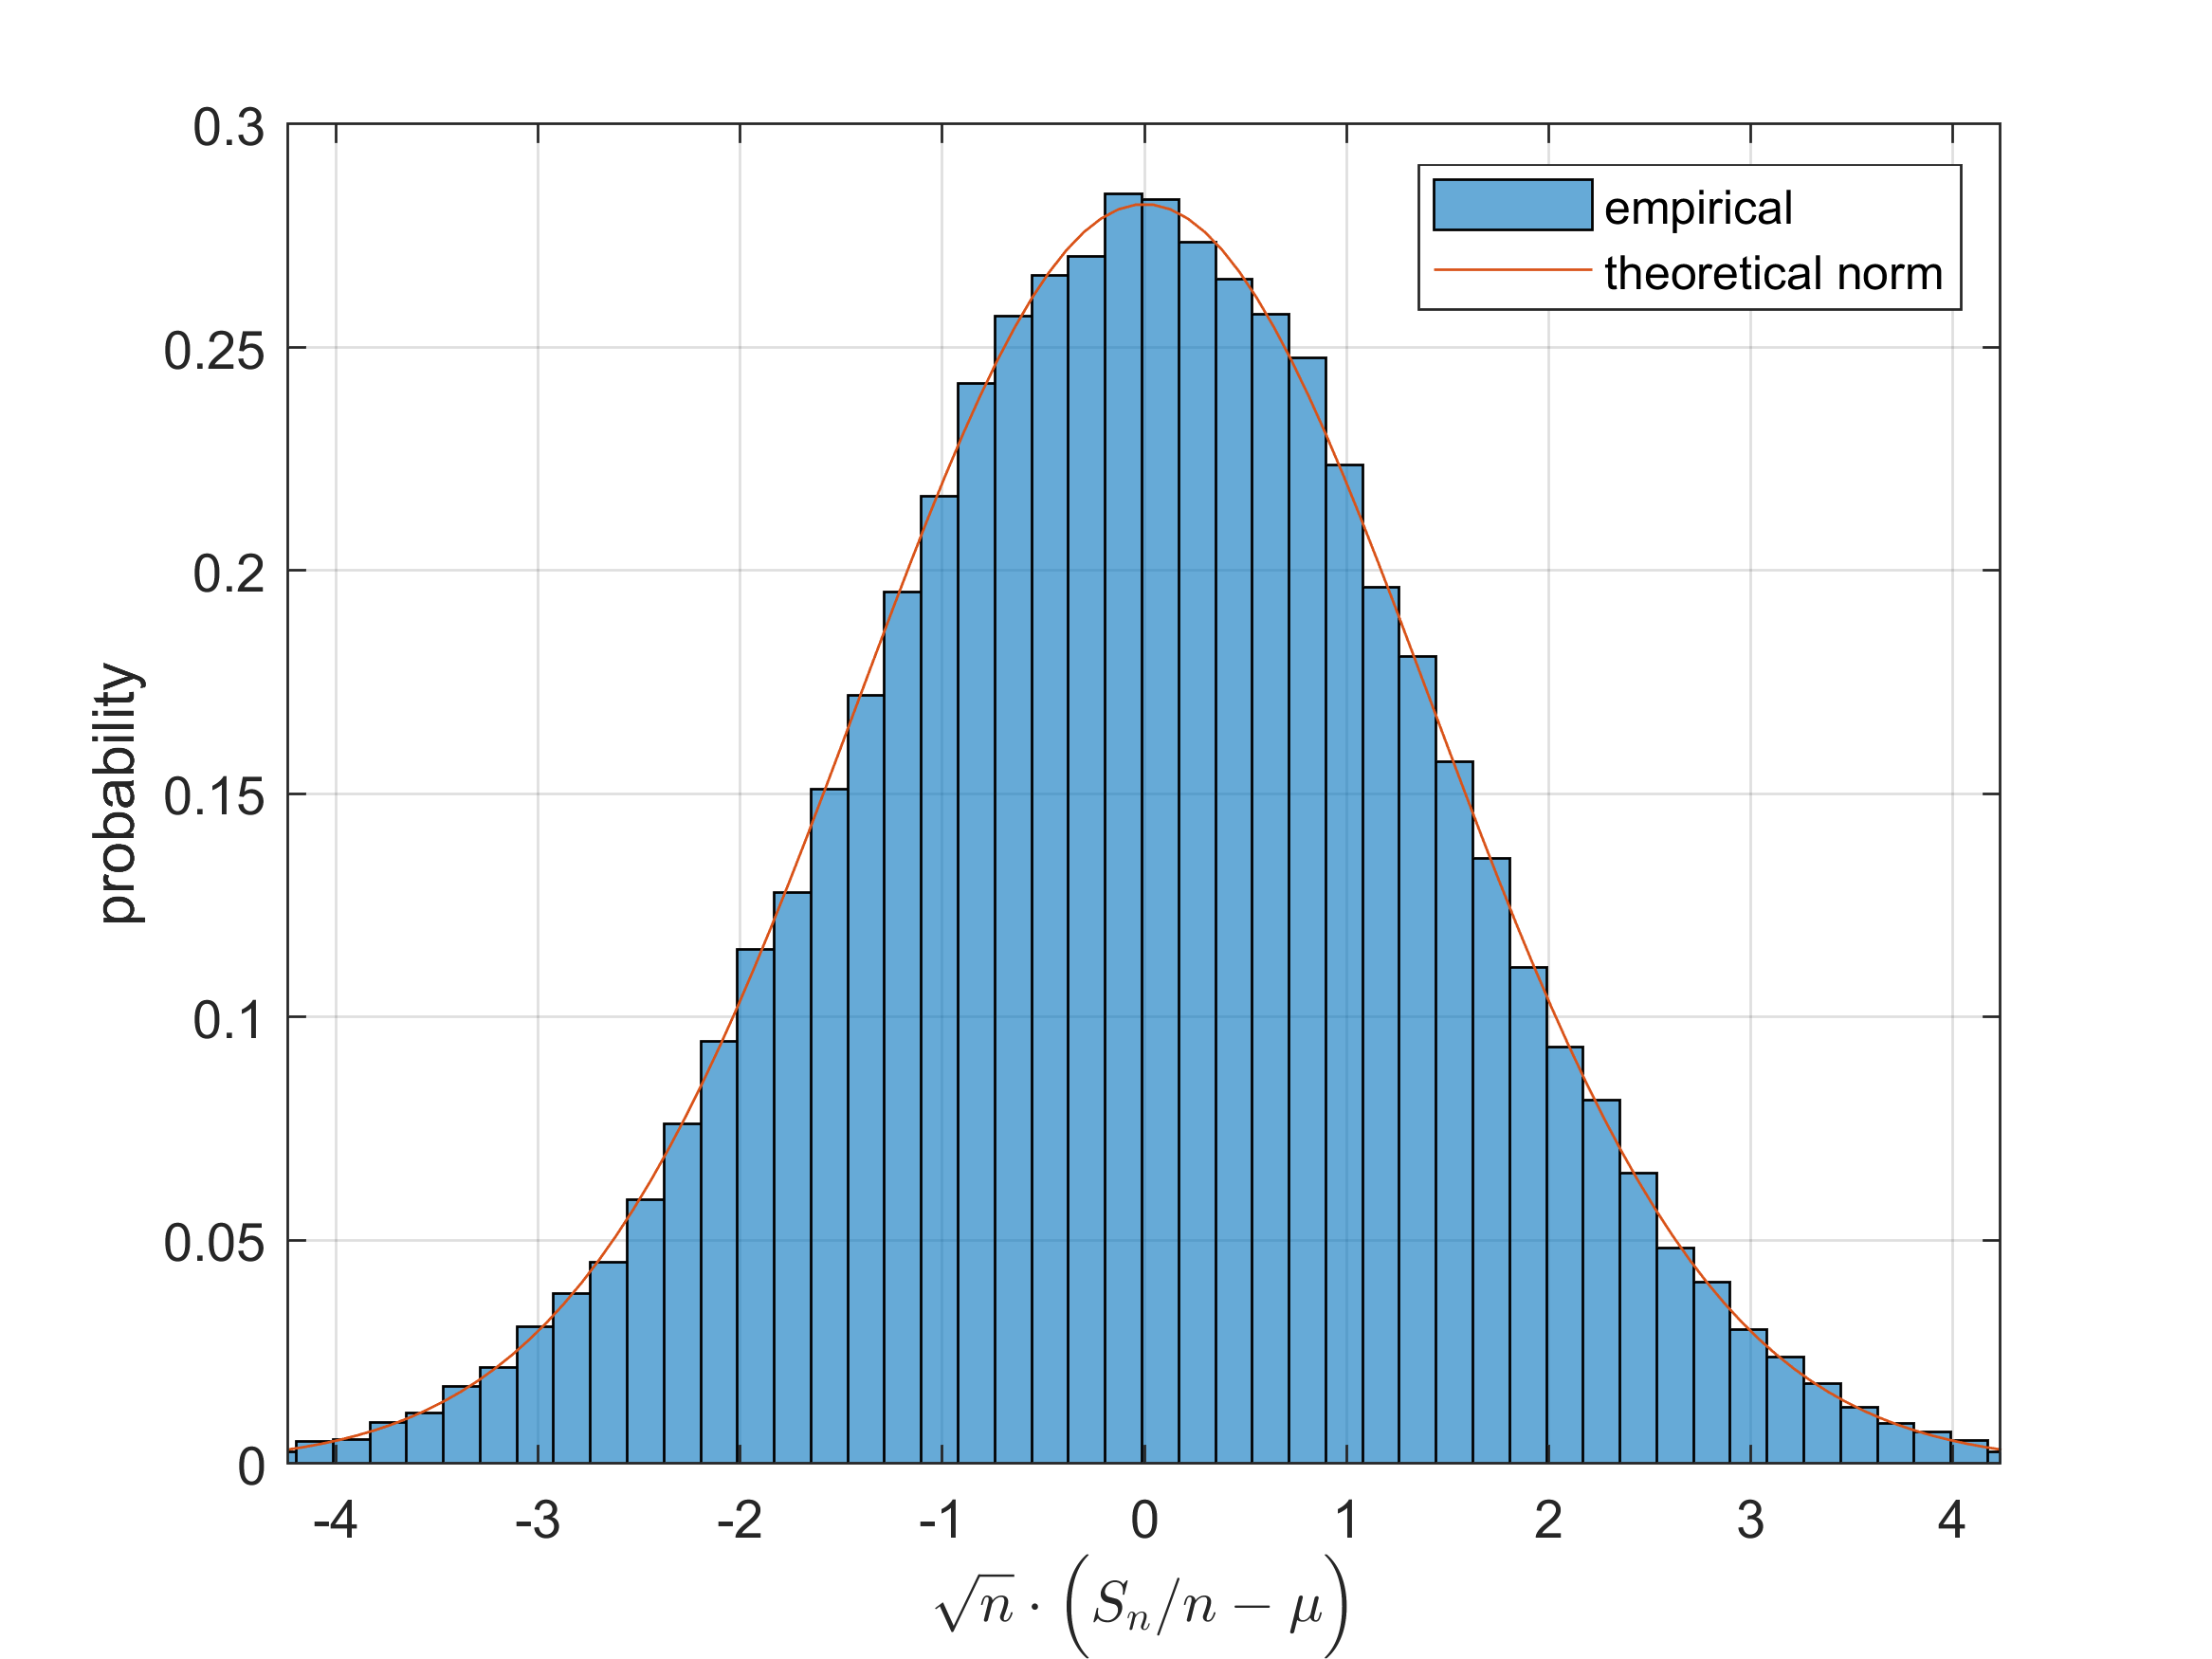
\includegraphics[width=0.6\textwidth]{../code/Task_5/pict/CTL_ex.png}
		\caption{\centering Демонстрация ЦПТ для $N=10^5$ статистик на основе выборок размером $n=10^3$
							\newline при $\mu=1, \sigma^2=2 $.}
    \end{figure}

\subsubsection{Пункт 2}
	
	Предположим, что наблюдается случайная величина $X\sim N(\mu,\sigma^2)$, а $(x_1,\ldots,x_n)$ --- 
	ее реализация. Тогда получим доверительные интервалы вида:
	$$
	\begin{gathered}
		\mu \in \left(\bar{x} - t_{\alpha/2, n-1}\frac{s}{\sqrt{n}};
							 \bar{x} + t_{\alpha/2, n-1}\frac{s}{\sqrt{n}}\right), \vspace{3mm} \\
		\sigma^2 \in \left(\dfrac{(n-1)s^2}{\chi^2_{\alpha/2, n-1}};\dfrac{(n-1)s^2}{\chi^2_{1-\alpha/2, n-1}}	\right),
	\end{gathered}
	$$
	где $\bar{x}=\sum\limits_{k=1}^{n}(x_k/n)$ --- выборочное среднее,
	$s^2 = \dfrac{1}{n-1}\sum\limits_{i=1}^{n}(x_i - \bar{x})$ --- выборочная дисперсия,	\newline
	$t_{\beta, n-1}$-  квантиль 
	распределения Стьюдента с $n-1$ степенью свободы для уровня значимости $\beta$, 
	$\chi^2_{\beta,n-1}$ -  $\beta$-квантиль $\chi^2$- распределения с $n-1$ степенью свободы.
	\newline 

	Доказательства можно найти в $\cite{conf_int}.$

\newpage
	\begin{figure}[h!]
		\centering
		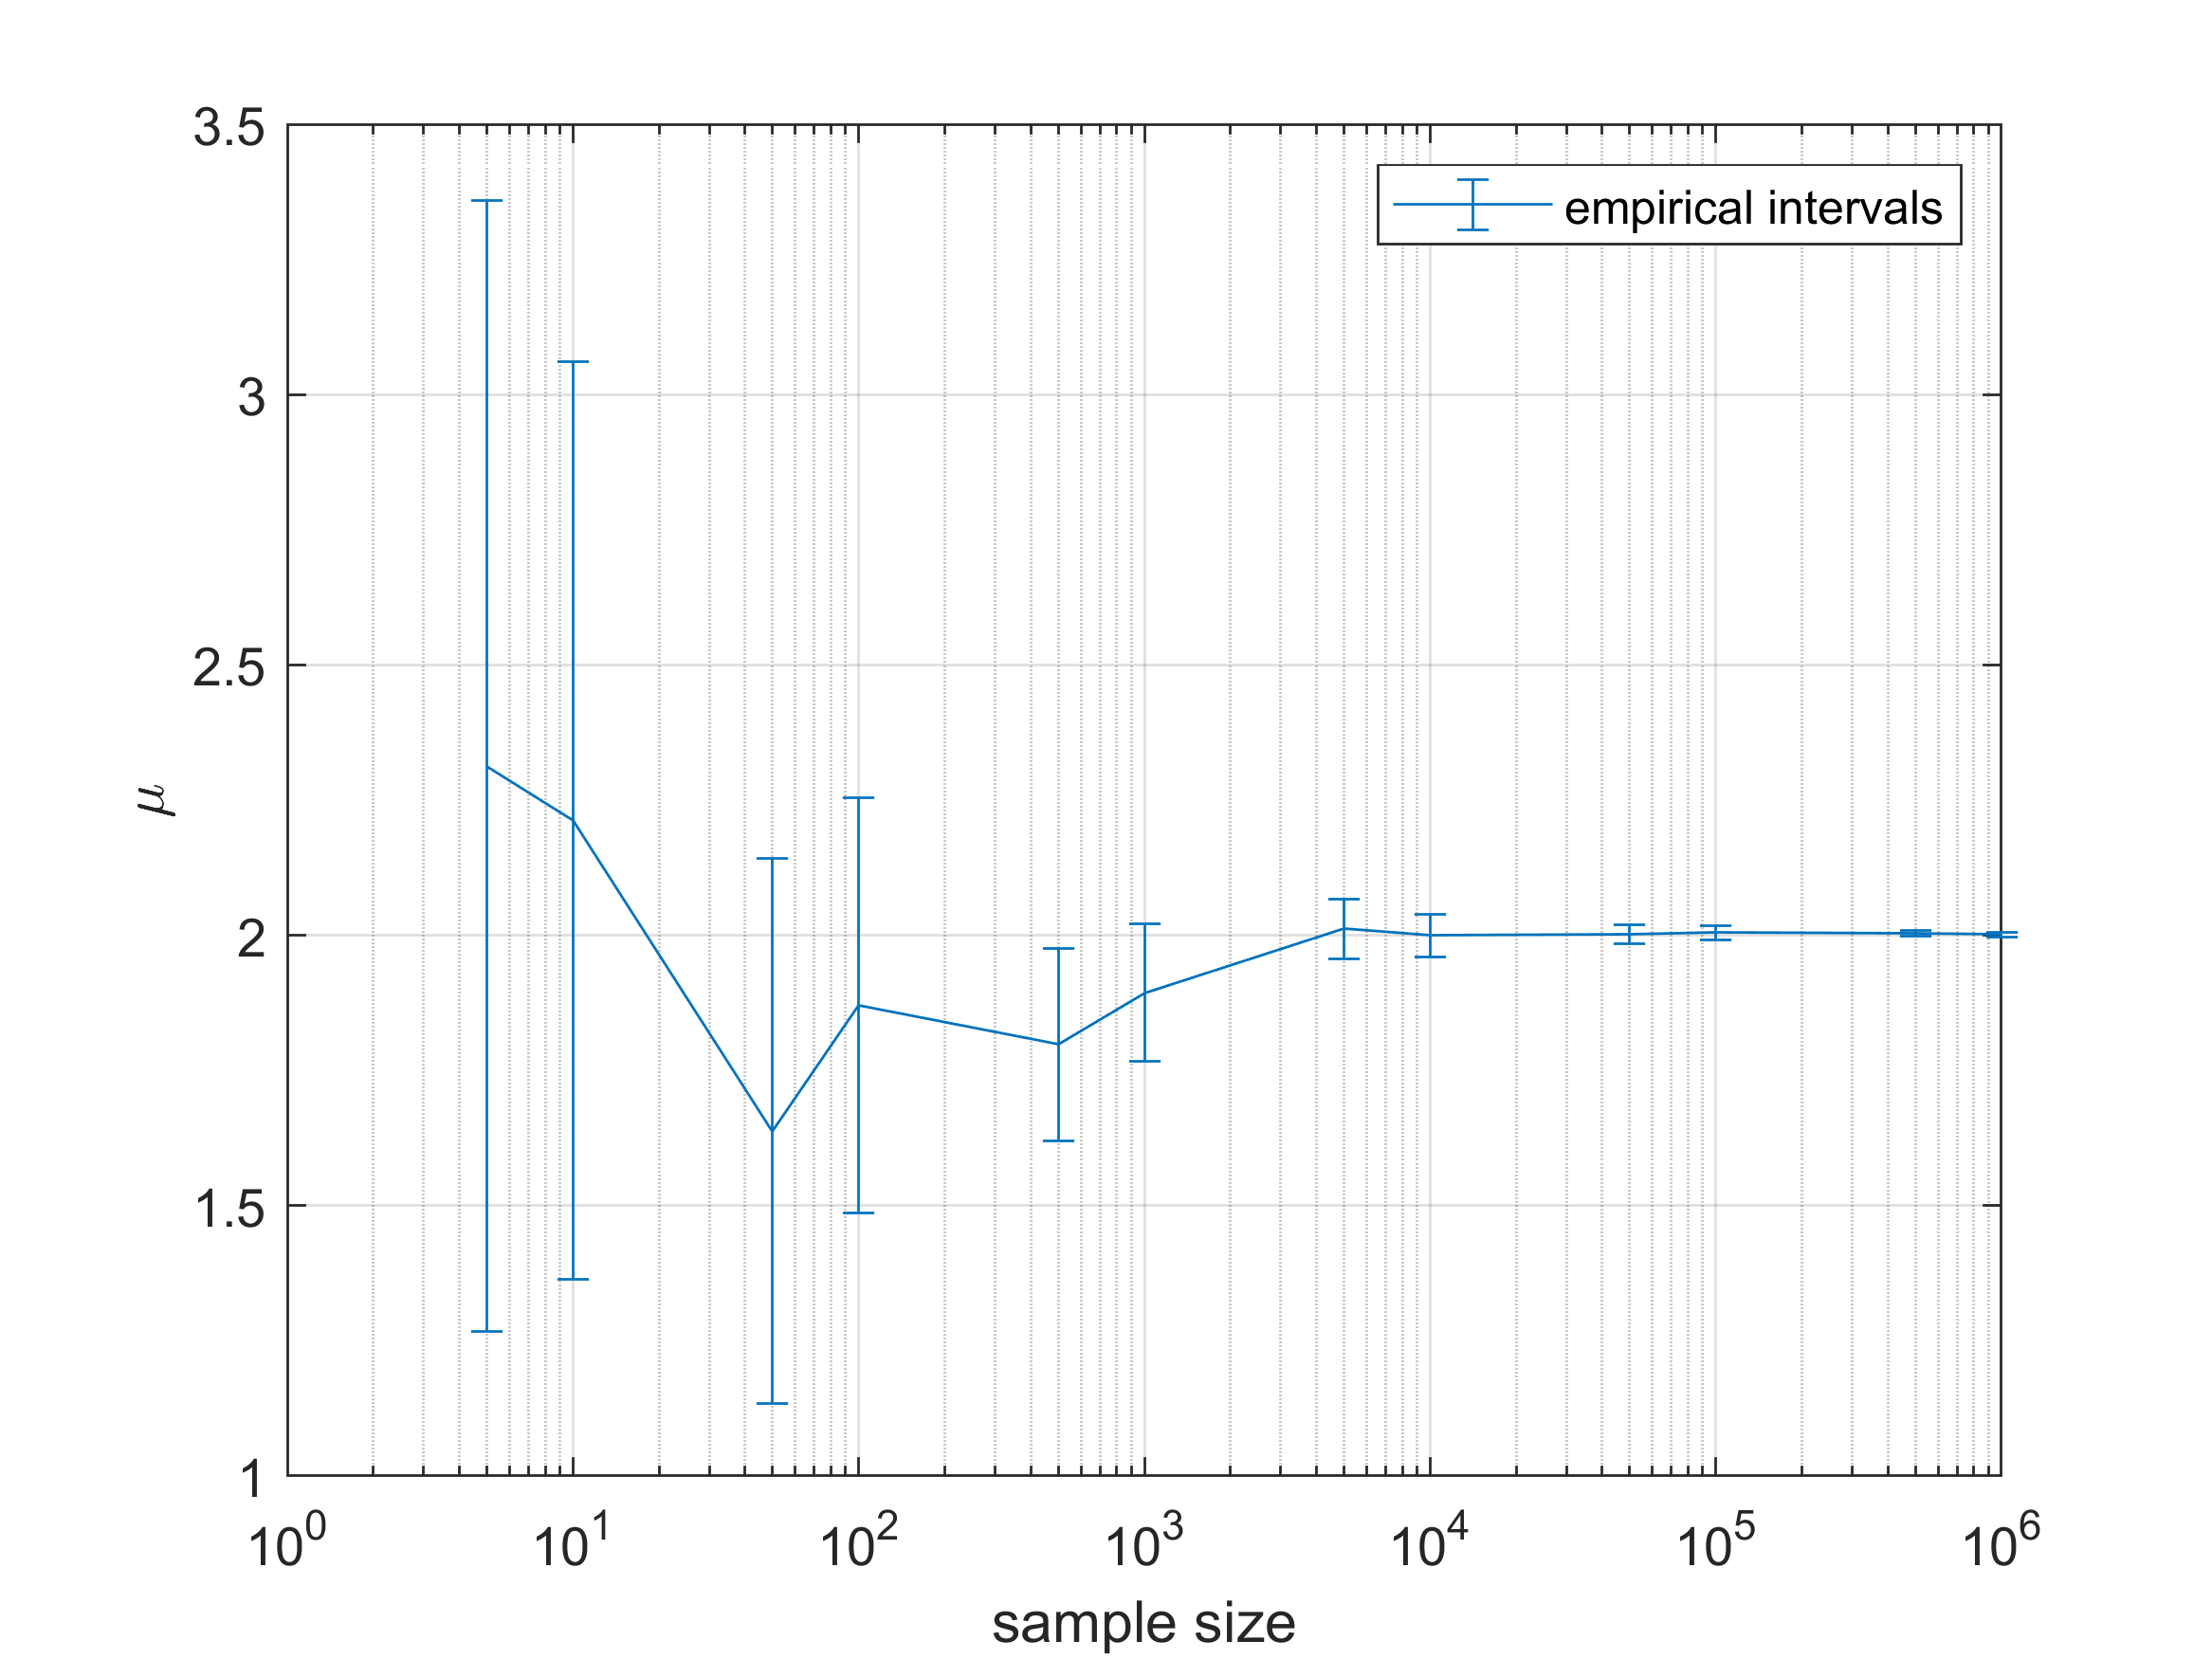
\includegraphics[width=0.6\textwidth]{../code/Task_5/pict/mu_conf.png}
		\caption{Доверительные интервалы для $\mu$ при $n=10^6$ 
						при $\mu = 2, \sigma^2  = 4$.}
    \end{figure}

	\begin{figure}[h!]
		\centering
		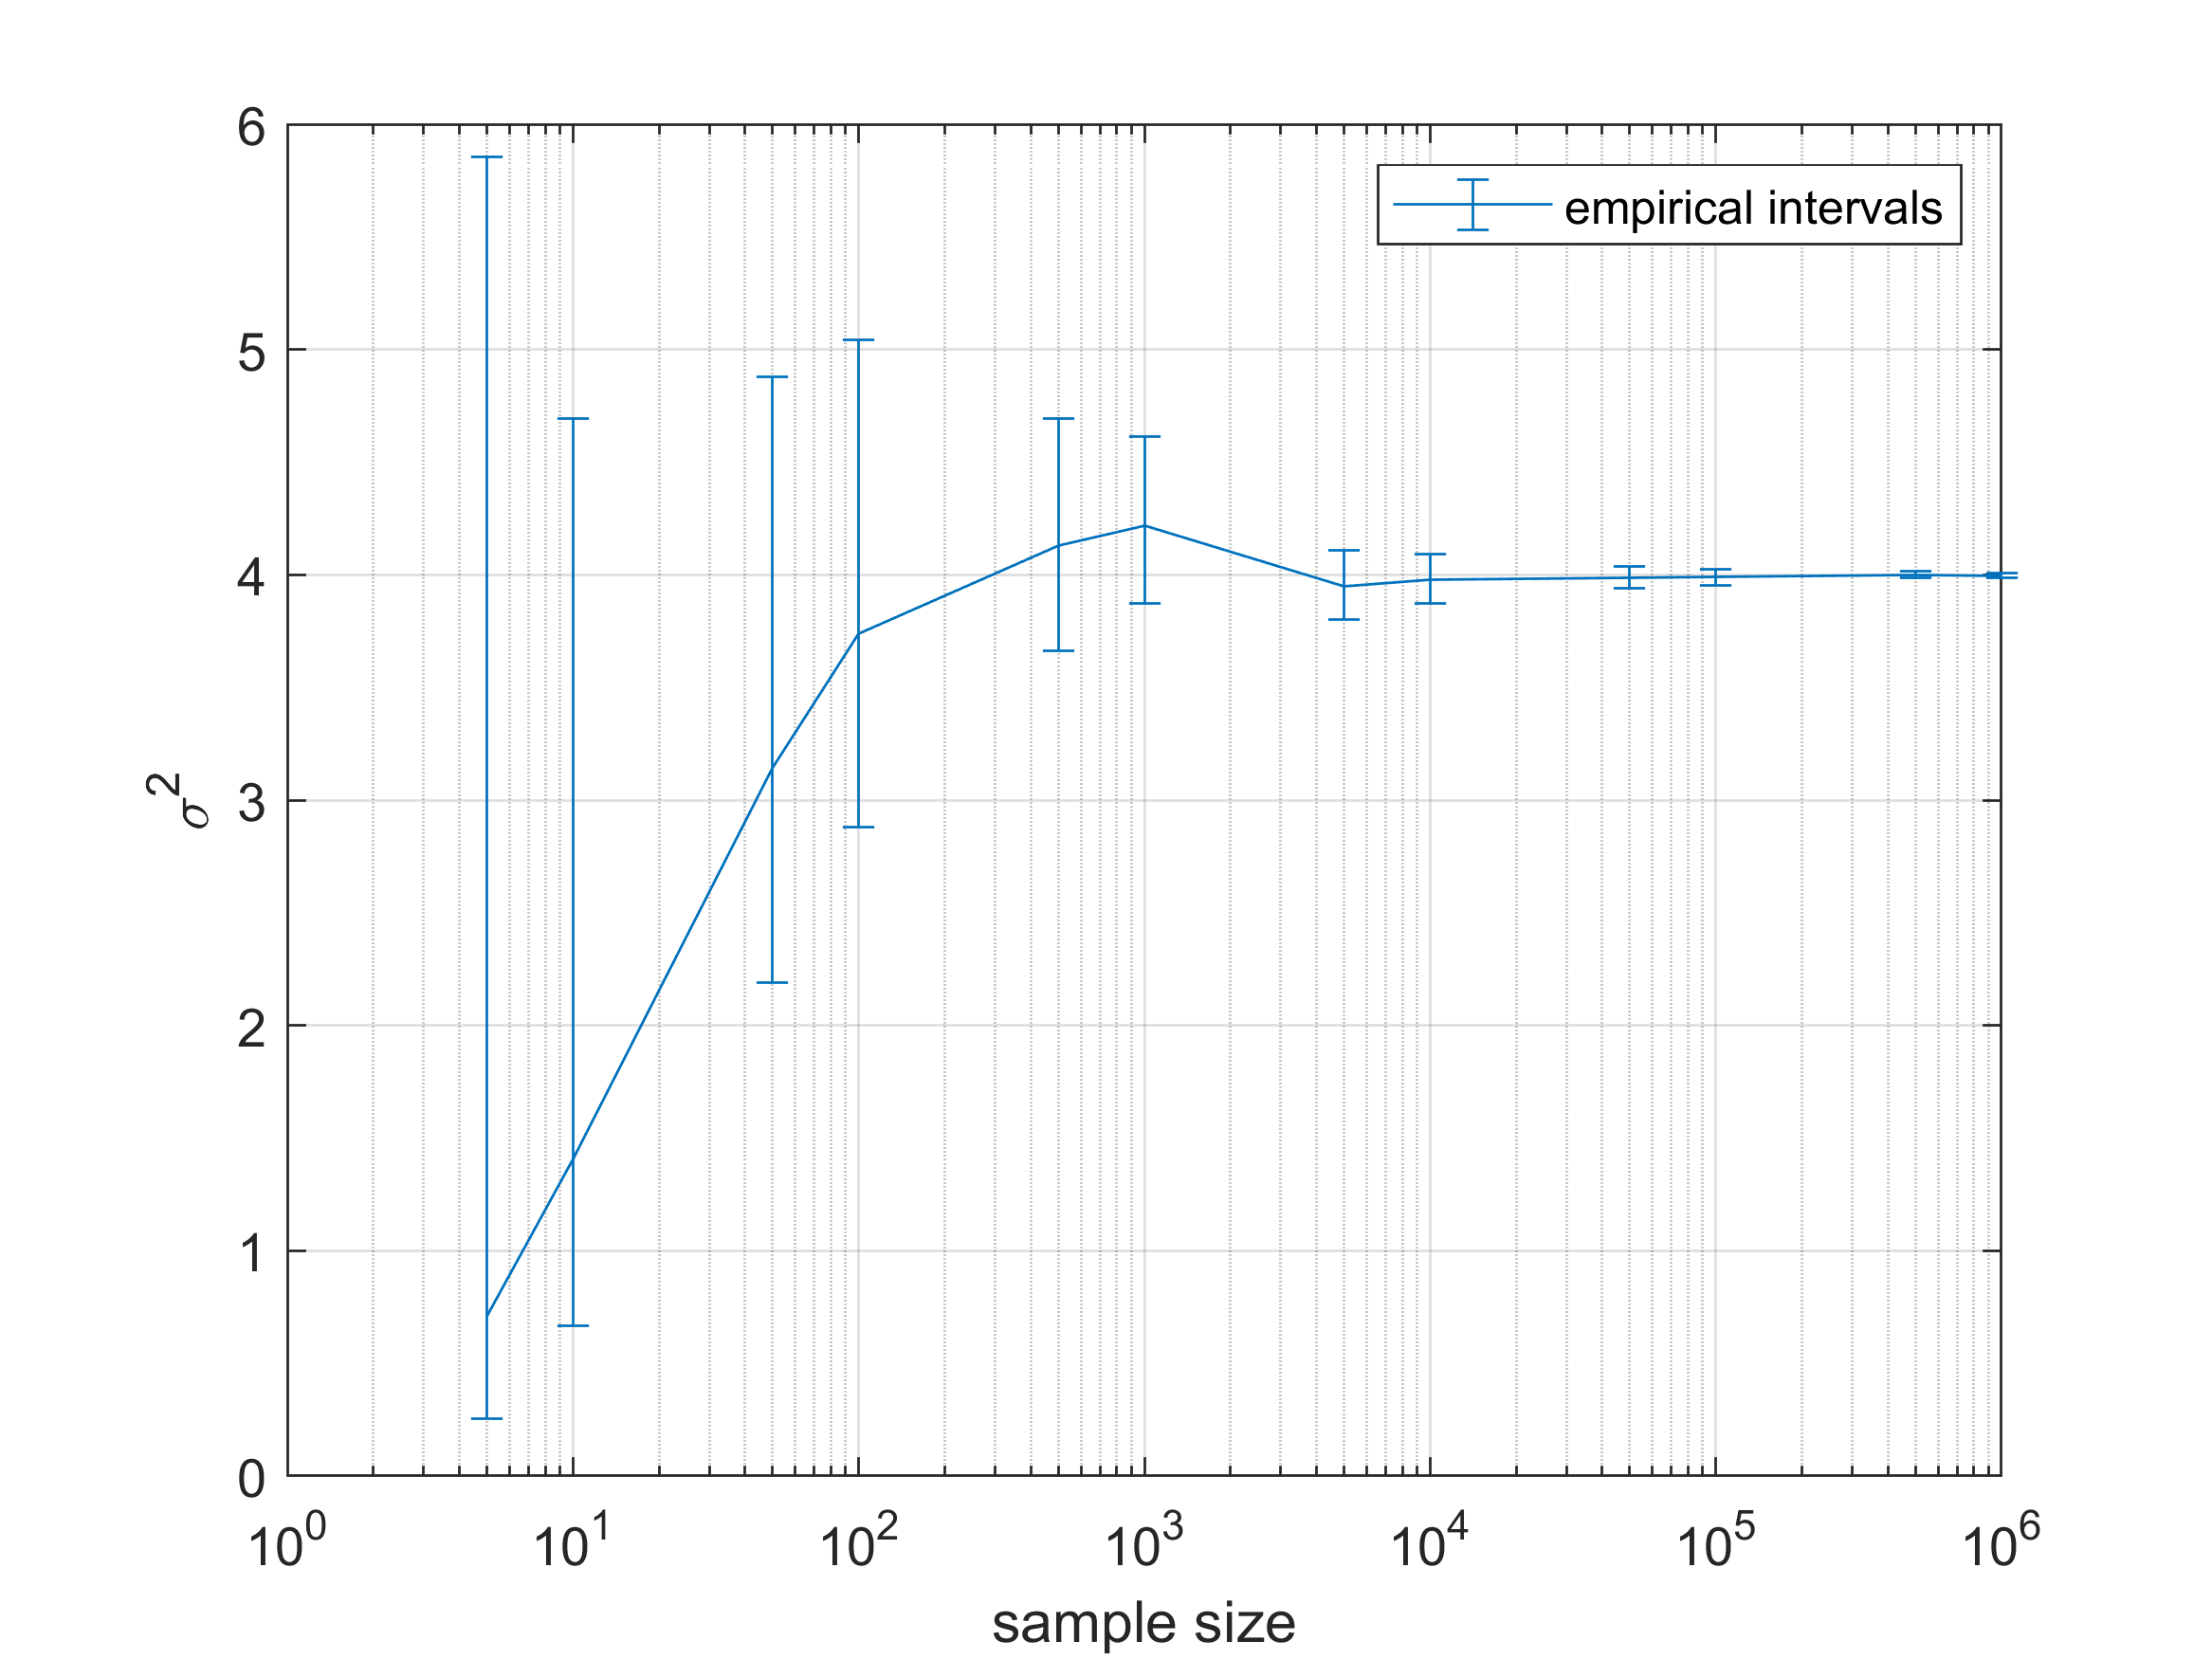
\includegraphics[width=0.6\textwidth]{../code/Task_5/pict/var_conf.png}
		\caption{Доверительные интервалы для $\sigma$ при $n=10^6$ 
						при $\mu = 2, \sigma^2  = 4$.}
    \end{figure}
	
\newpage
\subsubsection{Пункт 3}

	Пусть $X_i\sim K(a,b)$ имеет распределение Коши со сдвигом $a$ и масштабом $b$. 
	Найдем распределение $S_n/n$ при помощи аппарата характеристических функций.

	$$
		\begin{gathered}	
			\varphi_X(t) = \E (e^{itX}) = \int\limits_{\mathbb{R}} e^{itx}p(x)dx, \\
			\varphi_X(t)= \int\limits_{\mathbb{R}} \dfrac{e^{itx}}
																						{\pi b\left[ 1+\left(\frac{x-a}{b}\right)^2 \right]} dx	
									\Rightarrow \varphi_X(t) = \exp(i\a t -  \b|t|).
		\end{gathered} \vspace{2mm}
	$$
	\noindent
	Вспомним некоторые свойства характеристических функций:
	\begin{itemize}
		\item Для независимых случайных величин	$X_1, \ldots, X_n$ верно:
			$
				\varphi_{X_1+\ldots+X_n}(t) =\prod\limits_{k=1}^{n}\varphi_{X_k}(t),
			$
		\item 	$\varphi_{aX+b} = e^{itb}\varphi_X(at).$
	\end{itemize}
	Исходя из этого получим:
	$$
		\begin{gathered}	
			\varphi_{S_n}(t) = \prod\limits_{k=1}^{n}  \exp(i\a t - \b|t|) = \exp(i\a nt - \b n|t|), \\
			\varphi_{S_n/n}(t) = \varphi_{S_n}(t/n) = \exp(i\a t -  \b|t|) ,
		\end{gathered}
	$$
	что совпадает с исходным распределением Коши.

	Как мы можем наблюдать, распределения действительно совпали:
	
	\begin{figure}[h!]
		\centering
		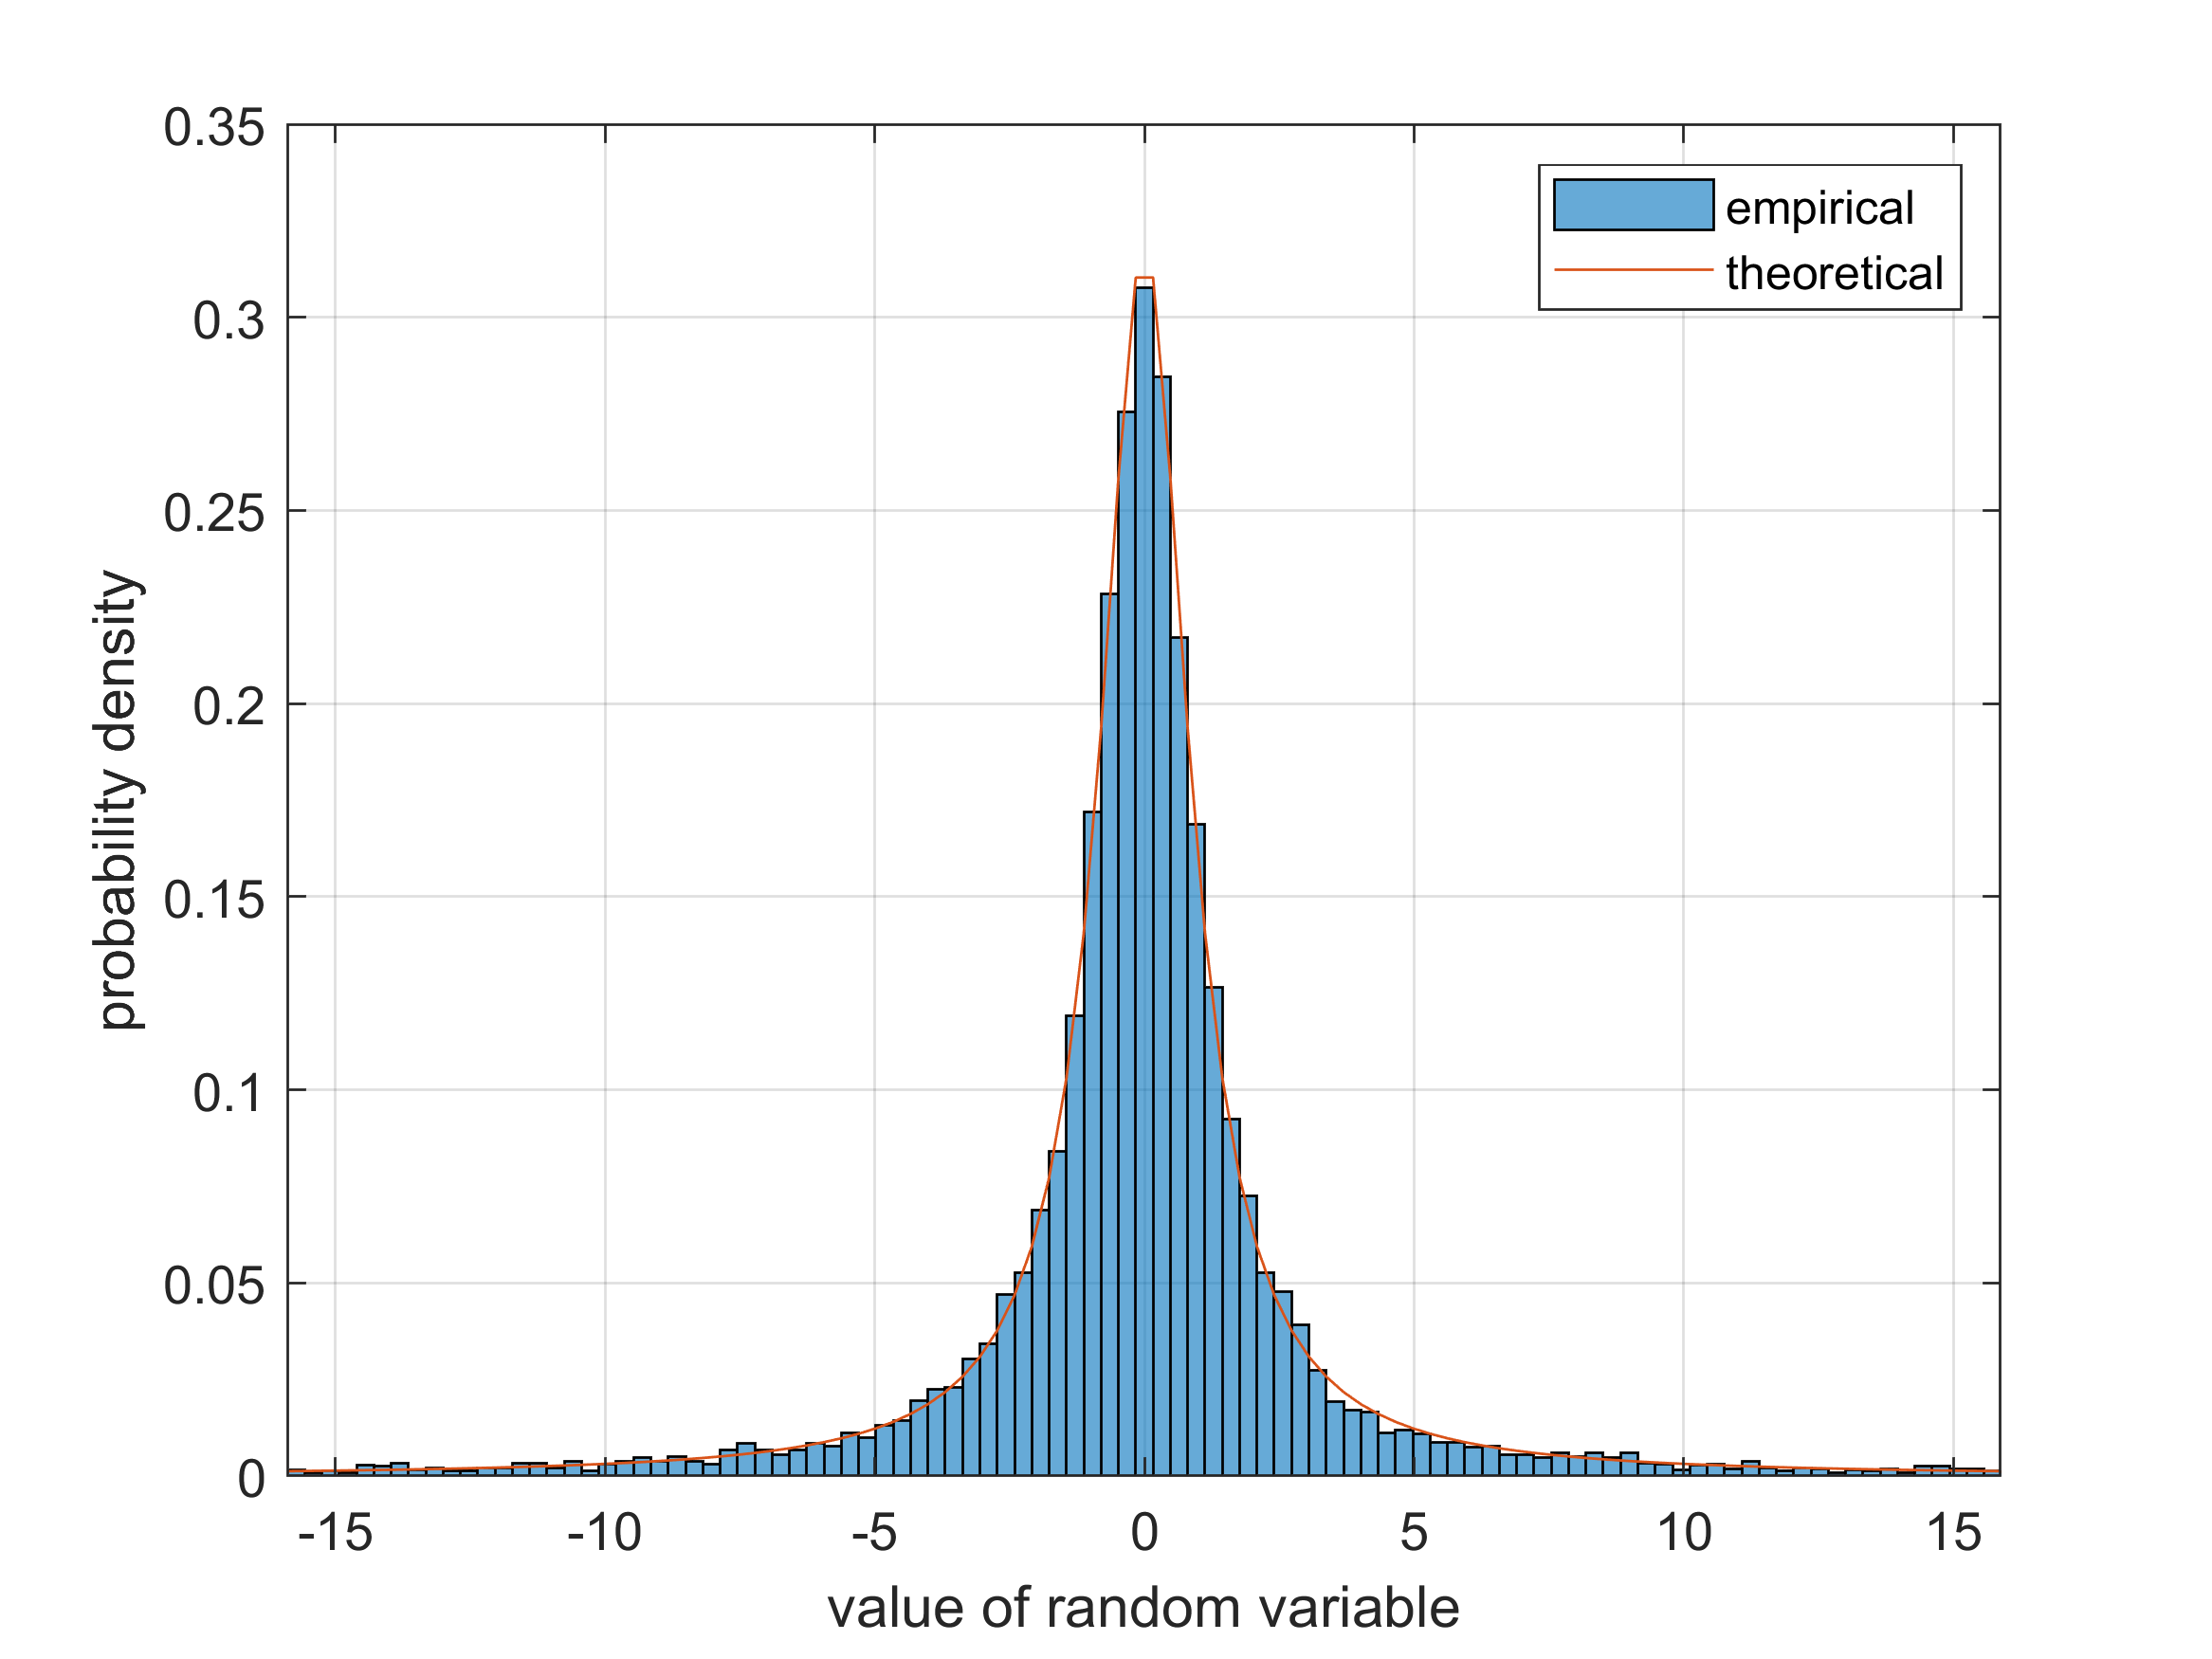
\includegraphics[width=0.6\textwidth]{../code/Task_5/pict/cauchy_sum_ex.png}
		\caption{Распределение $n=10^5$ искомых <<сумм>>, составленных из $10^3$ с.в., при $a=0, b=1$ .}
    \end{figure}

	\newpage
	У распределения Коши не существует математического ожидания, поэтому не выполняются условия 
	теоремы 5 и суммы $S_n/n$ ведут себя хаотично. Это видно на рисунке ниже:
	
	\begin{figure}[h!]
		\centering
		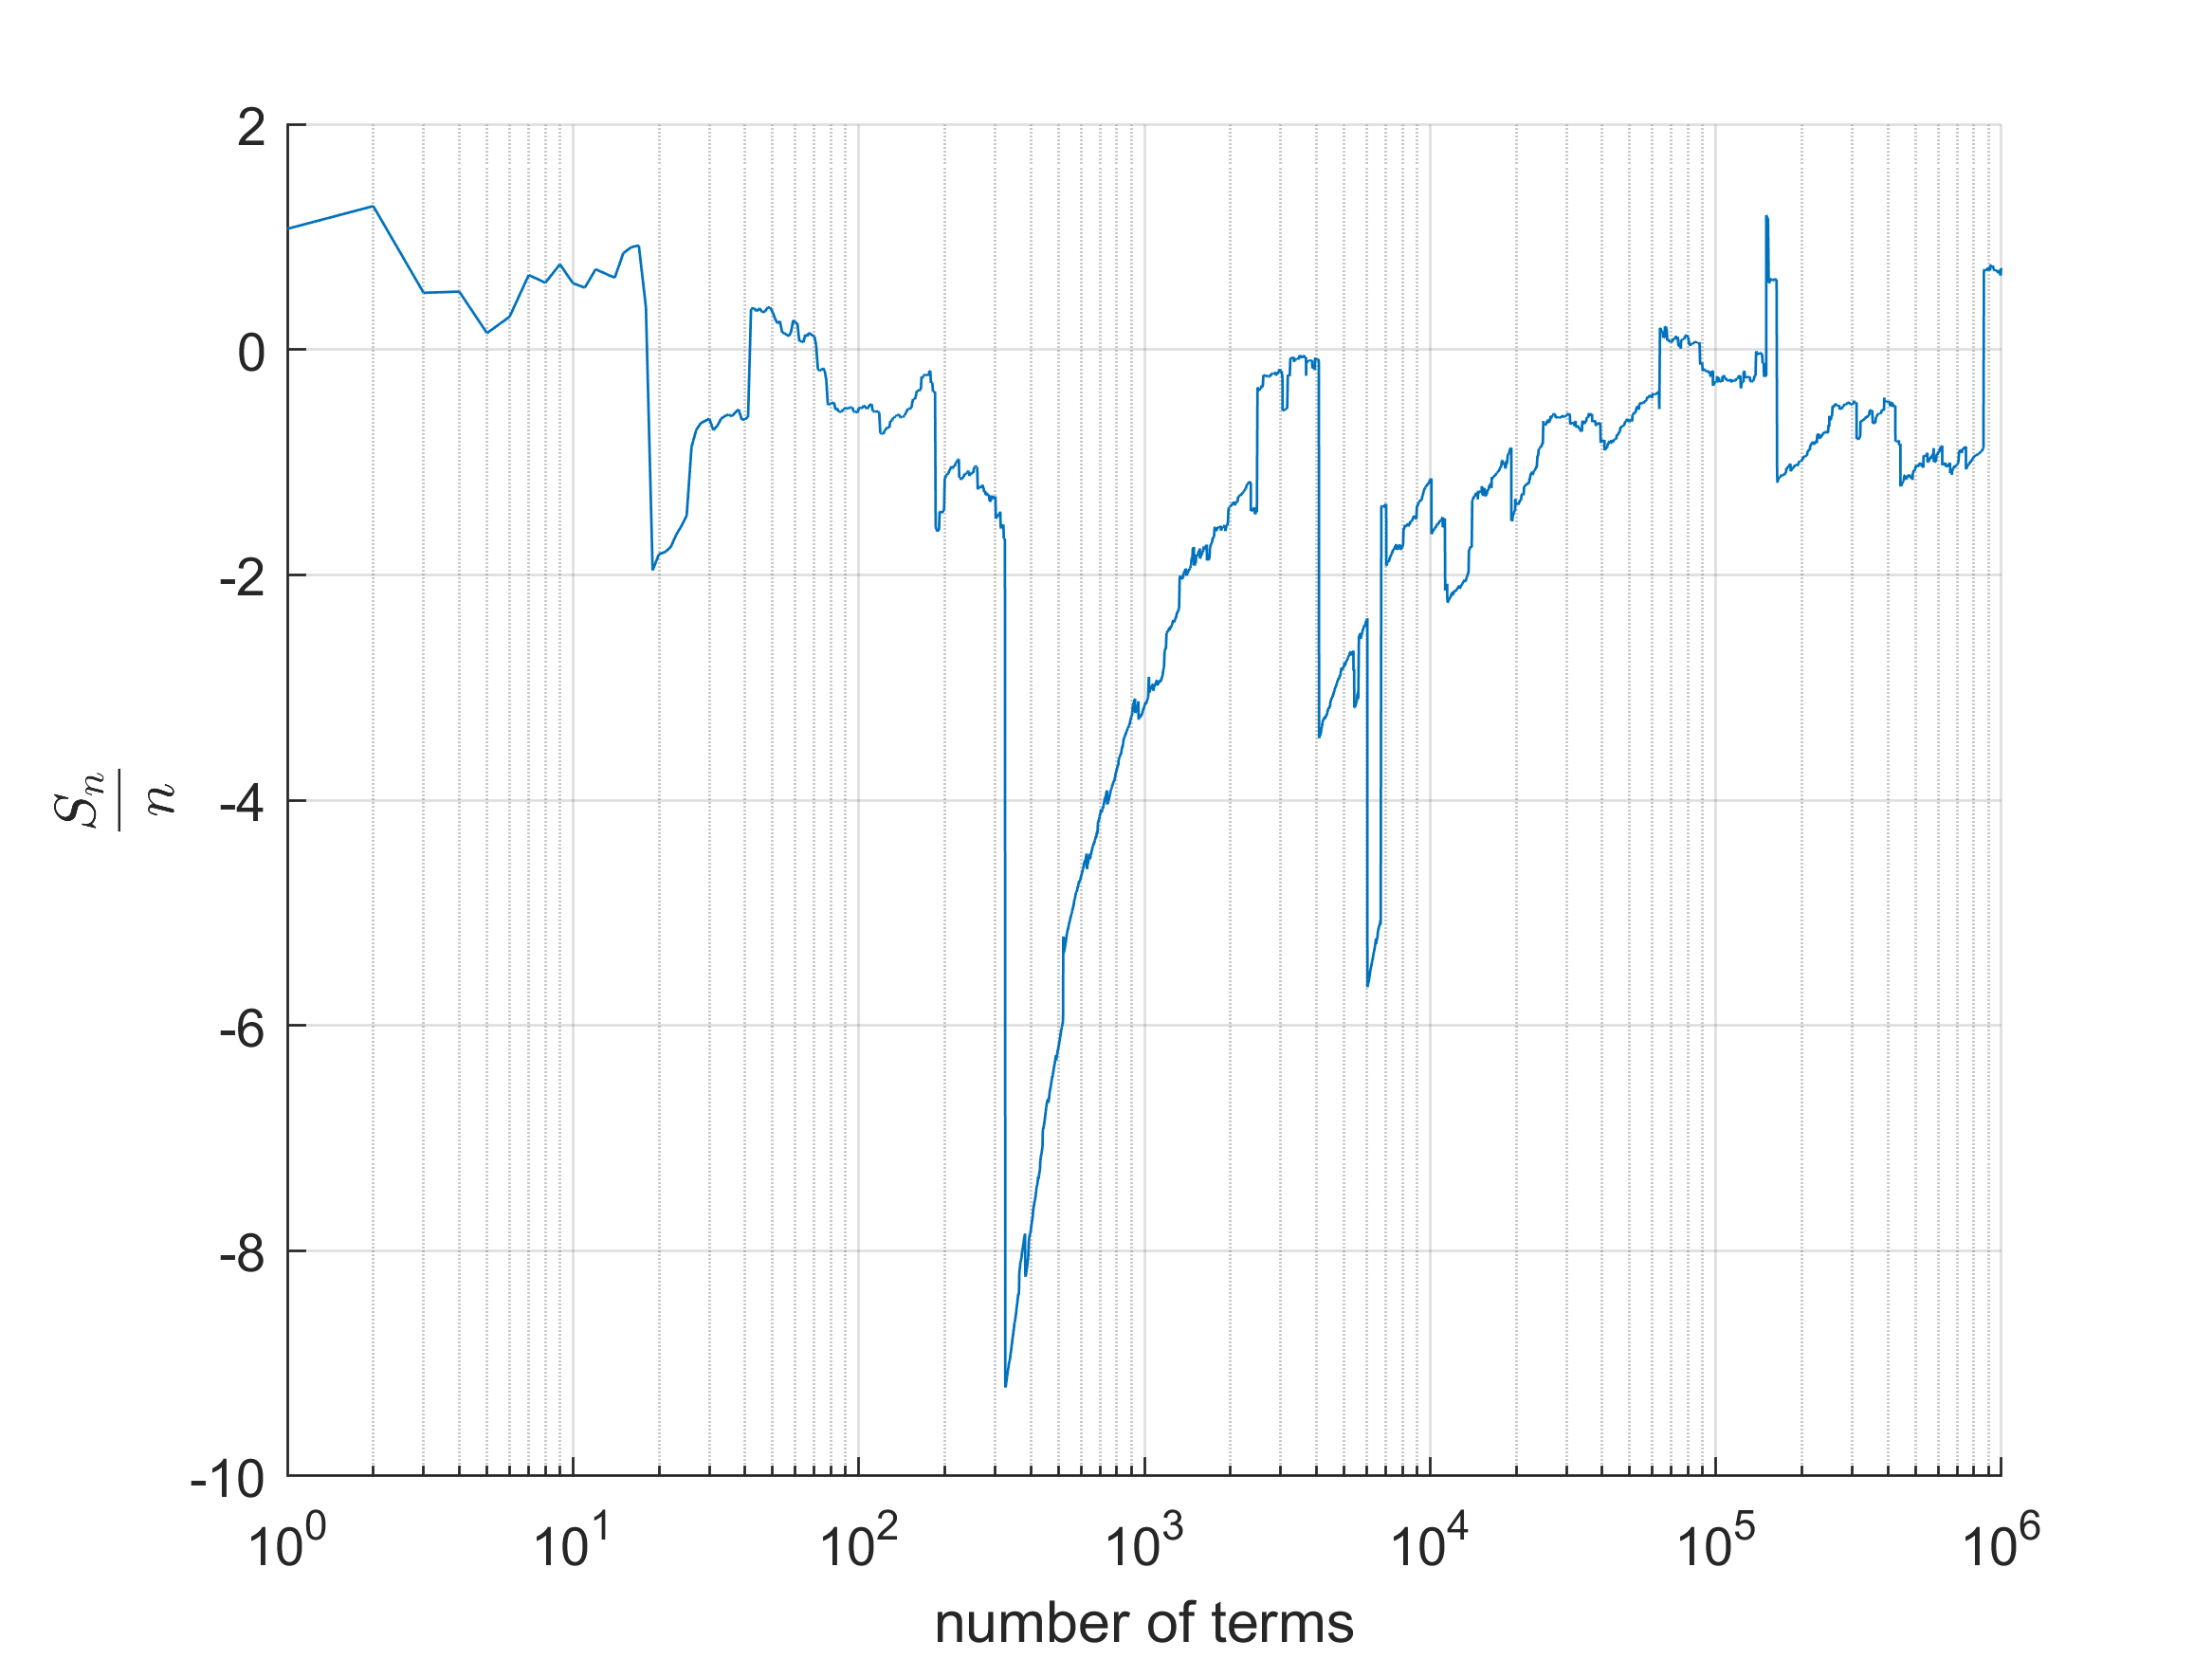
\includegraphics[width=0.6\textwidth]{../code/Task_5/pict/LLN_cauchy_ex.png}
		\caption{Демонстрация ЗБЧ для распределения Коши размером $n=10^5$ при $a=0, b=1$ .}
    \end{figure}
	
\section{Задание 6}

\subsection{Постановка задачи}
    \begin{enumerate} 
        \item Посчитать интеграл
        $$ 
            \int\limits_{-\infty}^{\infty} \int\limits_{-\infty}^{\infty}
                \ldots \int\limits_{-\infty}^{\infty}
            \frac{e^{-\Big(x_1^2+\ldots+ x_{10}^2 
                                + \frac{1}{2^7\cdot x_1^2 \cdot \ldots \cdot x_{10}^2 }\Big)}}
                    {x_1^2 \cdot \ldots \cdot x_{10}^2}
            d x_1 d x_2 \ldots d x_{10}
        $$
            \begin{enumerate}
                \item методом Монте-Карло
                \item методом квадратур, сводя задачу к вычислению собственного интеграла Римана
            \end{enumerate} 
        \item Для каждого оценить погрешность вычислений. 
    \end{enumerate}
\subsection{Решение задачи}
\subsubsection{Пункт 1}
	Перепишем исходный интеграл в виде:
	$$
		I = \int\limits_{-\infty}^{\infty} \int\limits_{-\infty}^{\infty}
                \ldots \int\limits_{-\infty}^{\infty}
            f(x_1, x_2, \ldots, x_{10}) g(x_1, x_2, \ldots, x_{10}) 
            d x_1 d x_2 \ldots d x_{10},
	$$
	где 
	$$
		f(x_1, x_2, \ldots, x_{10}) = \pi^5  \frac{e^{-\frac{1}{2^7\cdot x_1^2 \cdot \ldots \cdot x_{10}^2 }}}
                    {x_1^2 \cdot \ldots \cdot x_{10}^2}, \quad
		g(x_1, x_2, \ldots, x_{10})= \dfrac{1}{\pi^5} e^{-\left(x_1^2+\ldots+ x_{10}^2\right)}.
	$$
	Легко заметить, что функции $g(x)$ является совместной плотностью набора независимых нормально 
	распределенных случайных величин с параметрами 0 и 1/2. Таким образом, можно переписать 
	исходный интеграл в виде:
	$$
		I =\E [f(x_1, x_2, \ldots, x_{10})], \quad x_i \sim N\left(0,\frac{1}{2}\right).
	$$ 
	В силу ЗБЧ выборочное среднее будет стремится к математическому ожиданию:
	$$
		\dfrac{S_n}{n} = \dfrac{1}{n}\sum\limits_{i=1}^{n}f(x_1^k, x_2^k, \ldots, x^k_{10})
			 \xrightarrow[]{n\rightarrow \infty} \E [f(x^1_1, x^1_2, \ldots, x^1_{10})], 
				\quad x^k_i \sim N\left(0,\frac{1}{2}\right).
	$$
	Оценим погрешность метода Монте- Карло при помощи ЦПТ:
	$$
		\begin{gathered}
			\P \left( \left| \dfrac{S_n}{n}-I \right| < \varepsilon \right) = 
			\P \left( \left| \dfrac{S_n-In}{n} \right| < \varepsilon \right) =
			\P \left( \left| \dfrac{S_n-In}{\sigma \sqrt{n}} \right| < \dfrac{\sqrt{n}}{\sigma}\varepsilon \right) =\\= 
			\P \left(  - \dfrac{\sqrt{n}}{\sigma}\varepsilon  <
							 \dfrac{S_n-In}{\sigma \sqrt{n}} 
								< \dfrac{\sqrt{n}}{\sigma}\varepsilon \right) \approx
			\Phi\left(\dfrac{\sqrt{n}}{\sigma}\varepsilon\right) - \Phi\left(-\dfrac{\sqrt{n}}{\sigma}\varepsilon\right)=\\ = 
			2 \Phi\left(\dfrac{\sqrt{n}}{\sigma}\varepsilon\right)-1,
		\end{gathered}	
	$$
	где $\Phi(x)$ --- функция распределения стандартного нормального распределения. \newline
	Воспользовавшись таблицей квантилей и полученного квантиля $z_{\alpha}$ получим: 
	$$
		\varepsilon = \dfrac{z_{\alpha}\sigma}{\sqrt{n}}.
	$$
	Так как точное значение $\sigma$ неизвестно, будем пользоваться выборочной дисперсией:
	$$
		\sigma^2_n = \left( \dfrac{1}{n} \sum\limits_{i=1}^{n} f^2(\hat{x}_i) \right) - 
							   \left( \dfrac{1}{n} \sum\limits_{i=1}^{n} f(\hat{x}_i) \right)^2
	$$
	
	\begin{table}[h!]
	\begin{center}
		\begin{tabular}{|c|c|c|c|}
			\hline $N$ & Значение интеграла & Погрешность, \% & Время работы    \\ \hline
				$10^5$ & 123.14 & 0.074 & 0.017 \\ \hline
				$10^6$ & 125.1903 & 0.0234 & 0.1761 \\ \hline
				$10^7$ & 125.011 & 0.0074 & 1.7316 \\ \hline
				$10^8$ & 124.7931 & 0.0024 & 17.2832 \\ \hline
		\end{tabular}
		\caption{ \centering  Таблица значений интеграла, посчитанного методом Монте-Карло.}
	\end{center}
	\end{table}

\subsubsection{Пункт 2}
	Для подсчета интергала $I$ методом квадратур сделаем замену:
	$$
		x_i = \tg\left[ \dfrac{\pi}{2}t_i\right].
	$$
	Исходный интеграл примет следующий вид:
	$$ 
		I = \left( \dfrac{\pi}{2}\right)^{10}  \int\limits_{-1}^{1} \ldots \int\limits_{-1}^{1}
				\dfrac{ \exp\left\{ - \left( \sum\limits_{k=1}^{10}  \tg^2\left[ \frac{\pi}{2}t_k\right] +
														\frac{1}{2^7 \cdot \prod\limits_{k=1}^{10} \tg^2\left[ \frac{\pi}{2}t_k\right]}
											\right) \right\}}
						{\prod\limits_{k=1}^{10} \tg^2\left[ \frac{\pi}{2}t_k\right]\cdot
						 \prod\limits_{k=1}^{10} \cos^2\left[\frac{\pi}{2}t_k\right]} dt_1 \ldots d t_{10}.
	$$
	
	Воспользуемся методом прямоугольников. Для этого равномерно разобьем отрезок $[-1;1]$ на $N$ частей
	и будем считать величину :
	$$
		I_N = \dfrac{1}{N^{10}}\sum\limits_{k_1=1}^{N}\ldots \sum\limits_{k_{10}=1}^{N}
			f\left( \dfrac{2}{N}k_1-1, \ldots, \dfrac{2}{N}k_{10}-1 \right).
	$$ 
	Погрешность метода прямоугольников на равномерной сетке составляет:
	$$
		\varepsilon = \dfrac{\max|f''(\xi)|}{24}(1+1)h^2, 
	$$
	где $h$ --- диаметр разбиения. В нашем случае:
	$$
		\varepsilon = \dfrac{h^2}{12}\sum\limits_{i,j=1}^{10}\max\left|f''_{x_i,x_j}\right|, \quad h = \dfrac{2}{N}.
	$$
	
	Если внимательно посмотреть на интегрируемую функцию можно заметить, что она 
	\textbf{<<очень сильно симметричная>>}.
	\begin{enumerate}
		\item Функция зависит от только от значений $x_k^2$. 
					\newline Это значит, что нам достаточно будет просчитать только те
						точки, которые находятся в области, где $x_k>0 \forall k=1, [N/2]$. Пусть $[N/2] = L$.
						Обозначим значение интеграла по этой области за $I_{+}$. 
						Тогда значение исходного интеграла $I$ будет равно $I= 2^{10}I_+$. \newline
						Далее будем рассматривать только  $k: x_i^k >0$.
		\item Функция симметрична по любой паре переменных. \newline
				Это значит, что если мы поменяем местами $x_{k_1}$ и  $x_{k_2}$ в аргументах функции, 
				то значение самой функции у нас никак не поменяется. По-сути, перед нами встает 
				задача просчета функции только в тех точках, значение функции 
				в которых уникально. Поcле этого мы домножим это значение 
				на количество <<эквивалентных>> точек.
	\end{enumerate}

	Для начала поймем, как нам выделить <<уникальные>> точки.

	Идея заключается в том, что там необходимо подходящий положительный ортант в $\mathbb{R}^n$ рассечь 
	с помощью элементарных плоскостей симметрии \{например $x_1 = x_2$,
	т.к. $f(x_1,x_2,\ldots x_n) =  f(x_2,x_1,\ldots x_n)$\}. Тогда, выбрав одну из элементарных полученных фигур, 
	мы получим все <<уникальную область>>, т.е. не будет существовать значений функции, отличных от тех, 
	что были получены в этой области. 

	Проще всего это рассуждение представить в $\mathbb{R}^3$. В нем таким 
	уникальным множеством будет пирамида с вершинами, например, (0,0,0), (L,0,0), (L,L,0), (L,L,L).
	
	\newpage
	Опишем алгоритм перебора точек в уникальной области.\newline
	Представим себе матрицу $A$ размером $10\times L:$
	\begin{equation*}
			A = 
			\begin{array}{cccc}
			a_{1,1} & a_{1,2} & \ldots & a_{1,L}\\
			a_{2,1}  & a_{2,2} & \ldots & a_{2,L}\\
			\vdots  & \vdots & \ddots & \vdots\\
			a_{10, 1} & a_{10, 2} & \ldots & a_{10, L}
			\end{array}
	\end{equation*}
	
	Логично, что можно сделать просто 10 вложенных for от 1 до L, но мы сделаем чуть- чуть по -другому.

	Допустим, мы находимся в $i$-ой строке, т.е. в $i$-том вложенном for.
	Пусть мы начнем перебор с $j^i_0$-ого столбца, т.е. далее в 
	ходе <<перебора вглубь>> из $i$-ой строки будут использоваться только числа больше $j_0$. 
	Алгоритм выделения уникальных наборов из 10 чисел заключается в том, что в каждой следующей строке 
	перебора мы будем брать $j^{i+1}_0>=j^{i}_0$. Это логично, поскольку в противном случае 
	перебрав один раз пару $(\ldots, x^j_i, x^{j+1}_{i+1}, \ldots )$ нам не имеет смысла перебирать пару
	$(\ldots, x^{j+1}_i, x^{j}_{i+1}, \ldots )$, потому что значения функции на них совпадают.
	
		Идейно это можно объяснить так, что с увеличением каждого предыдущего индекса, размер
	 <<уникального подпространства>> для конкретного среза уменьшается.
	Можно проиллюстрировать эту трактовку для размерностей 2,3,4 и небольшого $L$.
	
	В связи с таким подходом, нам нужно понять какое количество точек эквивалентно каждой уникальной точке. 
	Пусть вектор из 10 чисел состоит из $m$ разных чисел, каждое из которых встречается $k_i$ раз.
	Тогда количество эквивалентных точек равно:
	$$
		n_{reps} = \dfrac{10!}{k_1!\ldots k_m!}.
	$$
	Псевдокод функции: \newline
	for $i_1$ = 1:10 

		 for $i_2$ = $i_1$:10 

			\ldots
				
			$f_{unique} = f(i_1, \ldots, i_{10})$; \{нашли уникальное значение функции\}

			$f_{sim} = 2^{10}* n_{reps} * f_{unique}$; \{сумма значений функции 
																						во всех симметричных точках \}
			
			\ldots

	end \newline
	end
		
	\begin{table}[h!]
	\begin{center}
		\begin{tabular}{|c|c|c|c|}
			\hline $N$ & Значение интеграла & Время работы    \\ \hline
				$$ 20 & 124.704 & 0.51648 \\ \hline
				$$ 32 & 124.8081 & 13.6501 \\ \hline
				$$ \textbf{40} & 124.8003 & 83.5463  \\ \hline
				$$ \textbf{50} & 124.8052 &  535.404 \\ \hline
				$$ \textbf{60} & 124.812 &  2675.4143 \\ \hline
		\end{tabular}
		\caption{ \centering  Таблица значений интеграла, посчитанного методом квадратур.}
	\end{center}
	\end{table}	
	
	В коде также реализован механизм уменьшения количества <<холостых>> проходов при малых
	номерах точек. <<Холостой>> проход --- это такой проход, 
	когда Matlab получает в качестве значения функции наскольно маленькое число, что кладет
	его равным точному нулю. Критическое значение в моем случае $eps \approx 10^{Х-800}$. 



\newpage
\section{Библиография}
	\begin{thebibliography}{99}
		\bibitem{smirnov} С.~Н.~Смирнов \textit{Лекции по стохастическому анализу}, 2019.
		\bibitem{feller} В.~Феллер \textit{Введение в теорию вероятностей и ее приложения}, 
			том 1. М: Мир, 1984.
		\bibitem{book_inv}  Н.~Ю.~Кропачева, А.~С.~Тихомиров \textit{Моделирование случайных величин}. 
						Издательство Новгородского Государственного Университета, 2004.
		\bibitem{conf_int}  Л.~Н~Фадеева, А.~В.~Лебедев   \textit{Теория вероятностей 
									и математическая статистика.} М.: Эксмо, 2010.
	\end{thebibliography}

\end{document}
